\documentclass[
hidelinks,
12pt, % The default document font size, options: 10pt, 11pt, 12pt
oneside, % Two side (alternating margins) for binding by default, uncomment to switch to one side
english, % ngerman for German
doublespacing, % Single line spacing, alternatives: onehalfspacing or singlespacing
%draft, % Uncomment to enable draft mode (no pictures, no links, overfull hboxes indicated)
%nolistspacing, % If the document is onehalfspacing or doublespacing, uncomment this to set spacing in lists to single
%liststotoc, % Uncomment to add the list of figures/tables/etc to the table of contents
%toctotoc, % Uncomment to add the main table of contents to the table of contents
%parskip, % Uncomment to add space between paragraphs
%nohyperref, % Uncomment to not load the hyperref package
headsepline, % Uncomment to get a line under the header
chapterinoneline, % Uncomment to place the chapter title next to the number on one line
%consistentlayout, % Uncomment to change the layout of the declaration, abstract and acknowledgements pages to match the default layout
]{MastersDoctoralThesis} % The class file specifying the document structure

\usepackage[utf8]{inputenc} % Required for inputting international characters
\usepackage[T1]{fontenc} % Output font encoding for international characters
\usepackage{subcaption}
\usepackage[belowskip=-15pt,aboveskip=0pt]{caption}
\setlength{\textfloatsep}{10pt plus 2.0pt minus 2.0pt}
\setlength{\intextsep}{10pt plus 2pt minus 2pt}
\setlength{\floatsep}{10pt plus 2.0pt minus 2.0pt}
\usepackage{mathpazo} % Use the Palatino font by default
\usepackage{booktabs}
\usepackage{colortbl}
\usepackage[ruled,vlined,linesnumbered,algochapter]{algorithm2e}
\usepackage[final]{pdfpages}
\usepackage{xcolor}
\usepackage{balance}
\usepackage{epigraph}
\usepackage{alltt} % for code snippet
\usepackage{listings}
\usepackage{hyperref}
\usepackage{amsmath,amsthm}
\usepackage{macros}
\usepackage{mathtools}
\usepackage{optidef}
\usepackage{float}
\usepackage{newtxmath}
\usepackage{polski}
\usepackage{tikz-cd}
\usepackage{flowchart}
\usepackage{tabularx}
\usepackage{enumitem}
% % Reduce spacing in toc
% \usepackage[titles]{tocloft}
% \setlength{\cftbeforechapskip}{5pt}
% Reduce spacing around section headers
\usepackage{titlesec}
\titlespacing*{\section}{0pt}{0pt}{5pt}
\titlespacing*{\subsection}{0pt}{2pt}{4pt}
\counterwithout{footnote}{chapter}
\usetikzlibrary{
  shapes,
  arrows.meta, % supersedes arrows
  calc,automata,positioning,fit,quotes}
  \tikzset{
  line/.style={draw, -Latex}
}
\tikzstyle{arrow} = [thick,->,>=stealth]
% \usepackage[square,numbers]{natbib}
% \bibliographystyle{abbrvnat}
\usepackage[backend=bibtex,style=numeric-comp,natbib=true,sortcites=true]{biblatex}
\usepackage[backend=bibtex,style=authoryear,natbib=true,backref=true]{biblatex} % use this line instead of the previous one if you want to use back references

\addbibresource{biblio.bib} % The filename of the bibliography


\usepackage[autostyle=true]{csquotes} % Required to generate language-dependent quotes in the bibliography

%----------------------------------------------------------------------------------------
%	MARGIN SETTINGS
%----------------------------------------------------------------------------------------

\geometry{
	paper=a4paper, % Change to letterpaper for US letter
	inner=4cm, % Inner margin
	outer=2.5cm, % Outer margin
	bindingoffset=.5cm, % Binding offset
	top=2.5cm, % Top margin
	bottom=2.5cm, % Bottom margin
    head=23.99748pt,
	%showframe, % Uncomment to show how the type block is set on the page
}

%----------------------------------------------------------------------------------------
%	THESIS INFORMATION
%----------------------------------------------------------------------------------------

\thesistitle{Manifold Structure of Artificial and Biological Neural Networks} % Your thesis title, this is used in the title and abstract, print it elsewhere with \ttitle
\supervisor{Dr/Pr. FirstName \textsc{LastName}} % Your supervisor's name, this is used in the title page, print it elsewhere with \supname
\examiner{Dr/Pr. FirstName \textsc{LastName}} % Your examiner's name, this is not currently used anywhere in the template, print it elsewhere with \examname
\degree{B.Sc (Hons)} % Your degree name, this is used in the title page and abstract, print it elsewhere with \degreename
\author{\textsc{Zhang} Liu} % Your name, this is used in the title page and abstract, print it elsewhere with \authorname
\addresses{} % Your address, this is not currently used anywhere in the template, print it elsewhere with \addressname

\subject{Mathematical, Computational and Statistical Sciences} % Your subject area, this is not currently used anywhere in the template, print it elsewhere with \subjectname
\keywords{manifold learning, neural computation, early primate vision, computer vision} % Keywords for your thesis, this is not currently used anywhere in the template, print it elsewhere with \keywordnames
\university{\href{https://www.yale-nus.edu.sg/}{Yale-NUS College}} % Your university's name and URL, this is used in the title page and abstract, print it elsewhere with \univname
\department{{}} % Your department's name and URL, this is used in the title page and abstract, print it elsewhere with \deptname
\group{{}} % Your research group's name and URL, this is used in the title page, print it elsewhere with \groupname
\faculty{{}} % Your faculty's name and URL, this is used in the title page and abstract, print it elsewhere with \facname

\AtBeginDocument{
%\hypersetup{colorlinks=false}
\hypersetup{pdftitle=\ttitle} % Set the PDF's title to your title
\hypersetup{pdfauthor=\authorname} % Set the PDF's author to your name
\hypersetup{pdfkeywords=\keywordnames} % Set the PDF's keywords to your keywords
\hypersetup{hypertexnames=true}

\setlength\abovedisplayskip{0pt}
\setlength\belowdisplayskip{0pt}
}


%%% TODO NOTES 
\usepackage{todonotes}
\def\frs#1{\todo[color=green!30]{\textbf{FS}:#1}}
\def\frsi#1{\todo[color=green!30,inline]{\textbf{FS}:#1}}

\begin{document}

\frontmatter

\pagestyle{plain} 

\begin{titlepage}
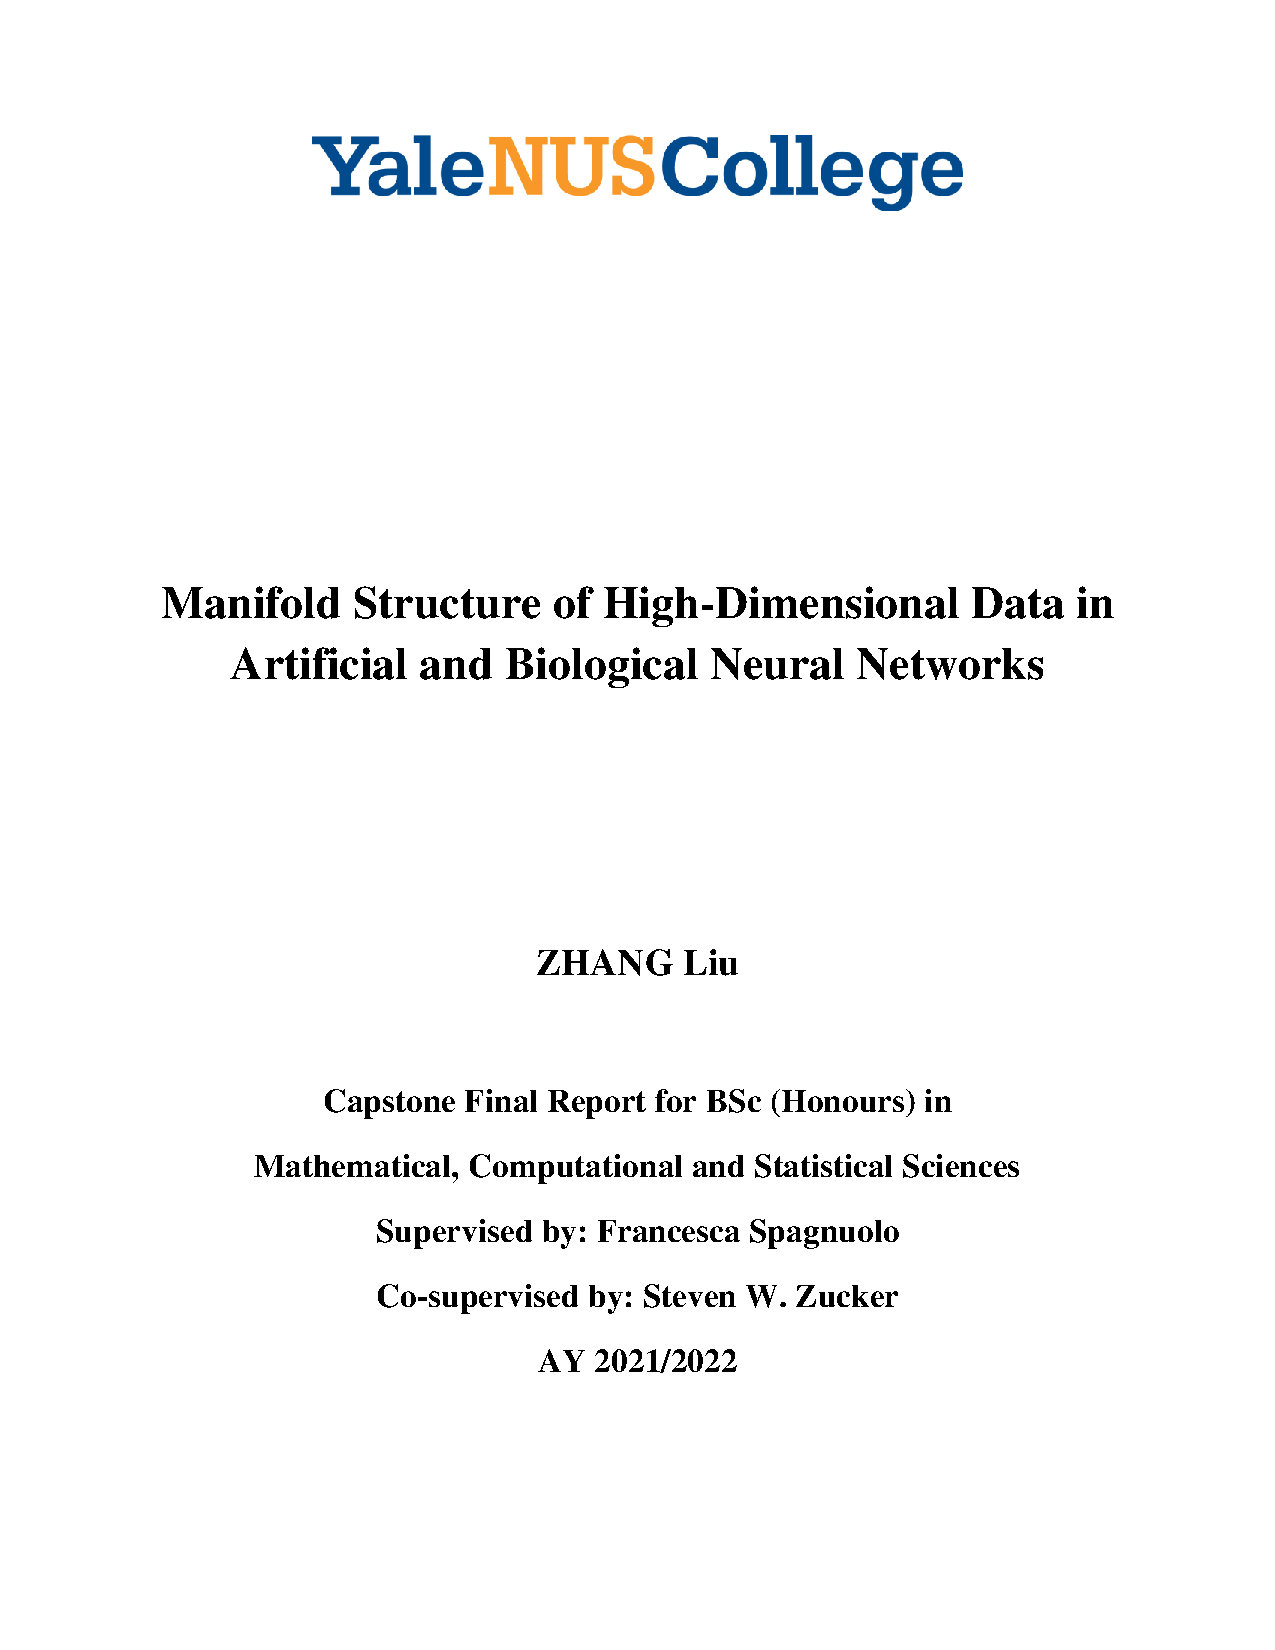
\includepdf[noautoscale=true]{capstone_titlepage.pdf}
\end{titlepage}

% \begin{abstract}
% \addchaptertocentry{\abstractname}
% \newpage 
% \centerline{\Huge Abstract}
\chapter{Abstract}
\textbf{Keywords: \keywordnames}

Our work builds on a long line of research aiming to develop more accurate computational models of the visual system. Despite decades of research, we have not fully understood the structure of neural circuits responsible for visual perception \cite{Gwilliams221630}. Additionally, among the computer vision (CV) community, there is a growing interest in investigating the limitations of the CV models by comparing them against biological vision. To this end, we seek to answer two specific open questions: First, how do CV models (VGG16 \cite{vgg16_simonyan_very_2015}, Vision Transformer \cite{vit_dosovitskiy_image_2021}, and Convolutional Recurrent Neural Network \cite{convrnn_shi_end--end_2015}) compare to biological vision, at retina and primary visual cortex (V1), in terms of their respective neural circuits\footnote{A neural circuit is a population of neurons interconnected by synapses to carry out a specific function when activated \cite{gerhard_neuroscience_2013}.}? Second, what specific mechanisms are important in causing such differences and/or similarities?

We first build the biological neural tensors using experimental neural spiking data and artificial neural tensors using numerical simulations on computer vision models (VGG16 \cite{vgg16_simonyan_very_2015}, Vision Transformer \cite{vit_dosovitskiy_image_2021}, and Convolutional Recurrent Neural Network \cite{convrnn_shi_end--end_2015}).
Using tensor CP decomposition, we obtain a manifold of neurons. The discrete data graph underlying the manifold then reflects both the neural circuit connections and the neurons' role in those circuits. By comparing the manifold structure of neurobiological networks in retina and V1 with that of computer vision models, we can make precise inferences about similarities and differences in their respective functional circuits. For the first time, we find that the underlying neural circuit of feed-forward computer vision models including CNN and ViT form disconnected network clusters, making them poor approximations of the visual cortex, contrary to popular belief. In order to model the highly connected neural circuits in the visual cortex, recurrent structure is likely necessary.

% \end{abstract}

% Since these groups are likely not independent, we use the non-linear dimensionality reduction method, diffusion maps, to infer a manifold of neurons.
% (represented by the discrete data graph underlying the continuous manifold) 
% groups  respond similarly to which stimuli input
%----------------------------------------------------------------------------------------
% CONTRIBUTIONS
%----------------------------------------------------------------------------------------

%https://ijast.org/credit-author-statement/

% In addition, code for displaying results in real-time, modules for managing servo overload, network latency and other factors were also written by the author.

% Reduce spacing in TOC

\begin{onehalfspacing}
\setcounter{tocdepth}{0}
\tableofcontents 
\end{onehalfspacing}



\mainmatter 
\pagestyle{thesis}

\chapter{Introduction} 
\label{chapter-intro} 

% 1. have a narrative!! 
% 2. make it absolutely clear that no one has done it before AND we have to figure this out!!

\section{Motivation and significance}
\label{intro-motivation}
In vision science, core object recognition has largely been modeled as a feed-forward process down the visual ventral stream \cite{dicarlo_how_2012}. First of such feed-forward models was Hubel and Wiesel's hierarchy model \cite{hubel_receptive_1962}, which classified the neurons in the visual cortex into simple and complex cells. This idea directly inspired the Neocognitron model \cite{fukushima_neocognitron_1980}, which in turn provided the basis for Convolutional Neural Networks (CNNs) \cite{alexnet},\cite{lenet}, which have become a dominant model in computer vision \cite{yamashita_convolutional_2018}. However, recent research starts to suggest that these feed-forward neural networks fail to model various key features in early primate vision  \cite{oreilly_recurrent_2013}, \cite{spoerer_recurrent_2017}, \cite{ricci_same-different_2018}, \cite{kietzmann_recurrence_2019}, \cite{van_bergen_going_2020}. In addition, across the different stages of early visual processing, the nature of neural computations vary drastically, particularly between the retina and the primary visual cortex (V1) \cite{dyballa_manifold_2021}. 

To this end, we seek to investigate the following related open questions:
\begin{itemize}[noitemsep, topsep=0pt]
    \item How do computer vision (CV) models (VGG16 \cite{vgg16_simonyan_very_2015}, Vision Transformer \cite{vit_dosovitskiy_image_2021}, and Convolutional Recurrent Neural Network \cite{convrnn_shi_end--end_2015}) compare to biological vision, at retina and primary visual cortex (V1), in terms of their respective neural circuits\footnote{A neural circuit is a population of neurons interconnected by synapses to carry out a specific function when activated \cite{gerhard_neuroscience_2013}.}?
     
    \item What specific mechanisms are important in causing such differences and/or similarities?
\end{itemize}

\begin{figure}[H]
\centering
\begin{subfigure}[b]{0.5\textwidth}
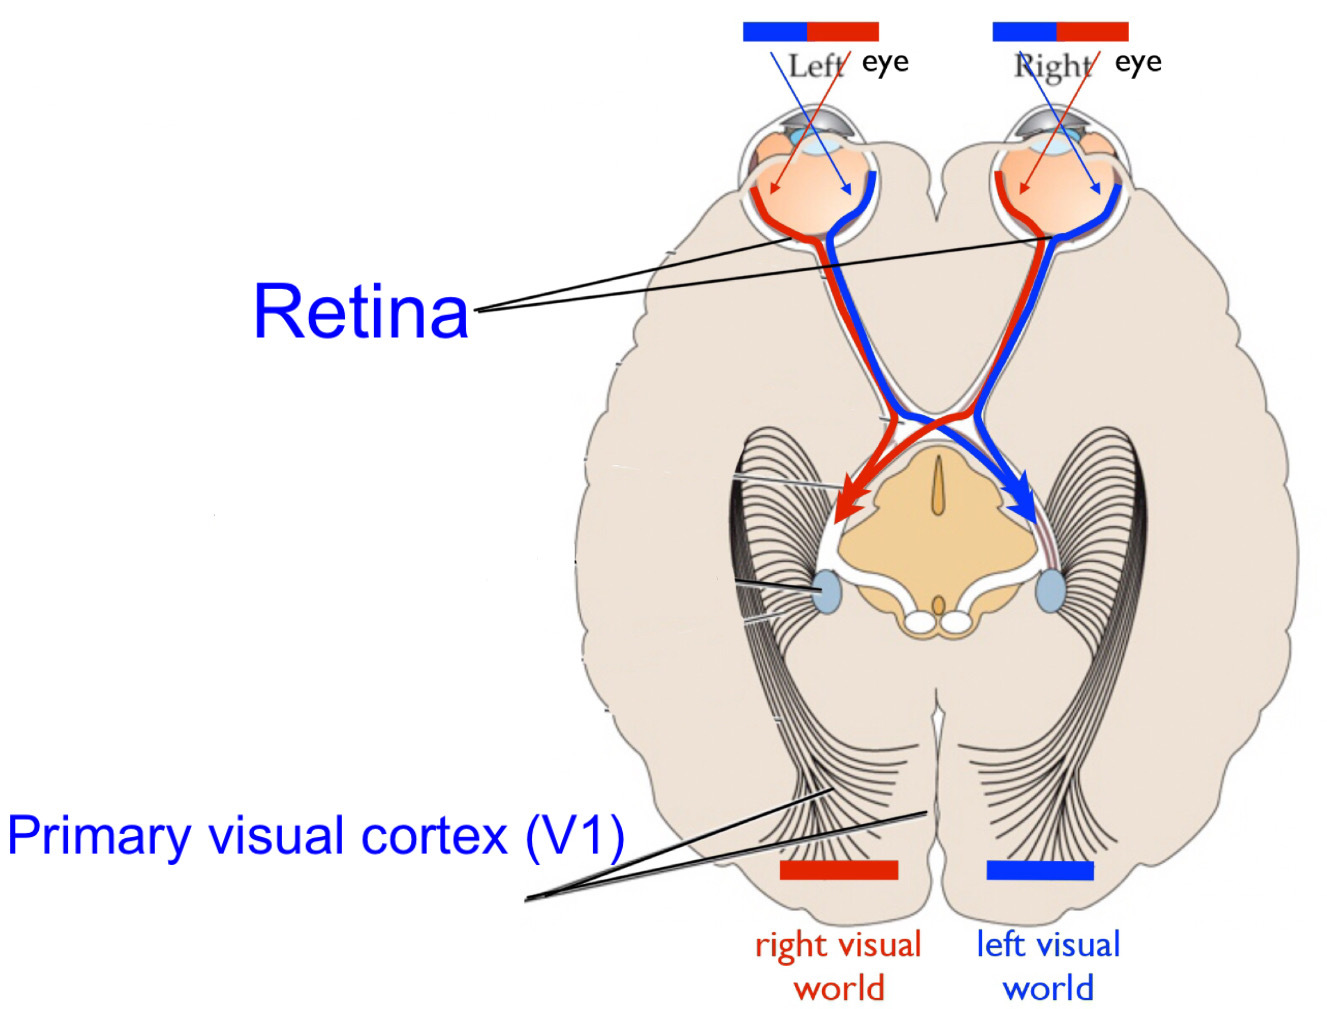
\includegraphics[width=\textwidth]{figures/intro/visual-pathway.jpg}
    \caption{Early visual pathway (from retina to LGN to V1). Adapted from \cite{pillow_vision_2022}}
\end{subfigure}
\hfill
\begin{subfigure}[b]{0.45\textwidth}
      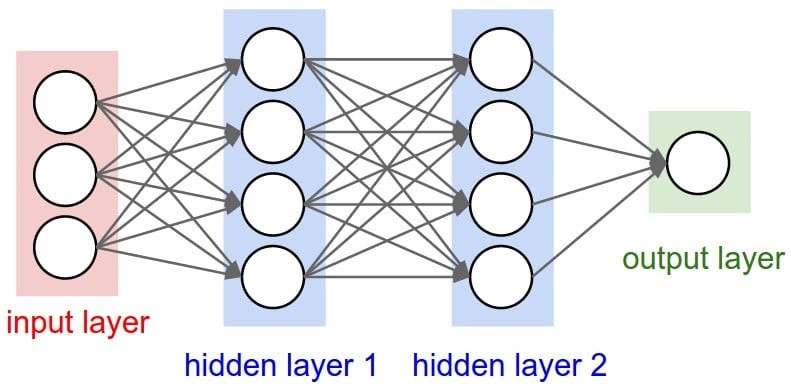
\includegraphics[width=\textwidth]{figures/intro/simple-ann.jpeg}
    \caption{Illustration for a simple ANN with two hidden layers.}
\end{subfigure}
\end{figure} 

\par The significance of answering these questions is two-fold. First, modeling the visual system has always been an important task in the field of neuroscience. Despite decades of research, we have not fully understood the structure of neural circuits responsible for visual perception \cite{Gwilliams221630}. Second, for the computer vision community, in addition to the existing research on explainability of computer vision models, there is a growing interest in investigating the limitations of these models by comparing them against biological vision. A growing number of research starts to reveal tasks that biological vision excels at while the state-of-the-art computer vision models fail. One notable example is that CNN is highly inferior to human vision in solving visual problems that involve relational reasoning \cite{glorot-bengio-difficulty}, such as recognizing same-different relations in images \cite{ricci_same-different_2018}, categorizing images based on the constituent parts \cite{visual-categorization}, and comparing features in images  \cite{cnn-human-abstraction}. The hope is that with a rigorous comparison, we can discover the specific mechanisms responsible for certain desired features of biological vision that the current computer vision models are lacking and adapt those mechanisms into computer vision models with relevant computational constraints in mind.
% Some of the concrete examples of recent breakthroughs in computer vision that takes inspiration from biological vision are reviewed in section \ref{brain-inspired}. 

% ([to-do] Specific to our project, why would computer vision models learn from biological vision? what is the advantage? does recurrence helps vision??)

% In the field of AI, more sophisticated models of the visual system could inspire new computational algorithms in solving increasingly demanding computer vision tasks. In fact, research in computer vision has taken many inspirations from neuroscience. In LeCun, Bengio, \& Hinton's seminal work on deep learning (\cite{lecun_deep_2015}), they stated that ``ConvNets have their roots in the Neocognitron," which was one of the earliest computational models of the visual system. 
\section{Framework of comparison}
\label{intro-framework}
Both subjects of our study, artificial and biological neural networks, are instances of black box problem where the underlying function is unknown. The best approach to investigate the internal structure of a black box system is to probe the system with some input and record the output:
\begin{figure}[H]
    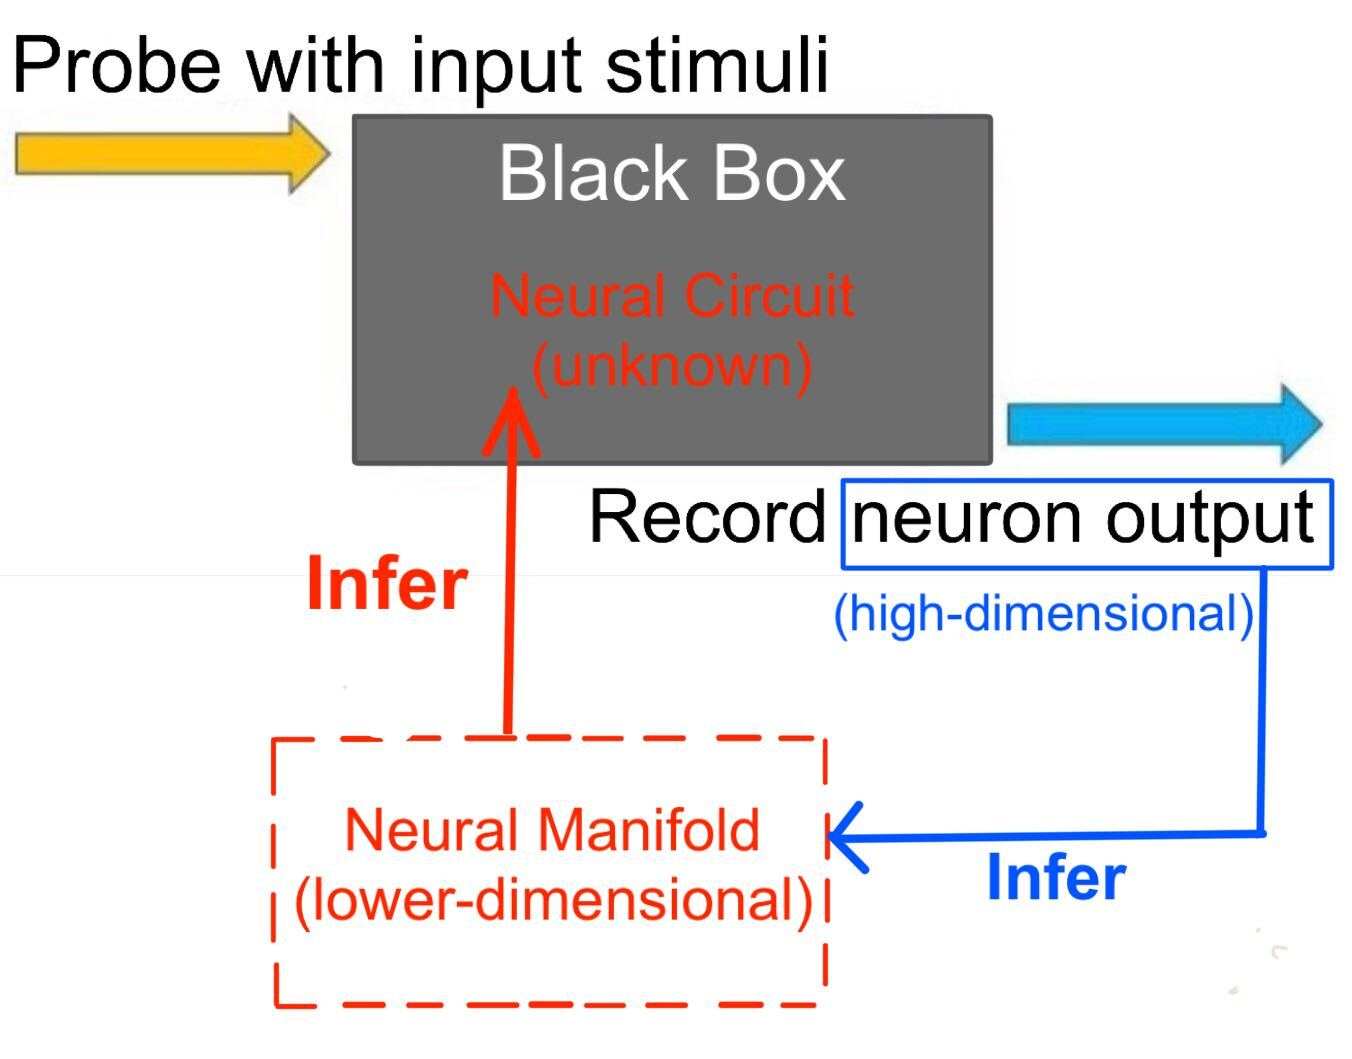
\includegraphics[width=0.85\textwidth]{figures/intro/black-box.jpg}
    \caption{Illustration of the black box problem.}
\end{figure} 

Applying this approach to our problem, we compare the neural circuits of artificial and biological neural networks (both unknown \textit{a priori}) by comparing the neural output from each network when given the appropriate input. Since the neural output is encoded in high-dimensional representations, it is impossible to analyze the organization of neurons directly based on their responses to visual stimuli. For this reason, we need to infer an intermediate lower-dimensional representation, which we call ``neural manifold" and will be our basis for comparison. 

\subsection{ \textit{What is a neural manifold?}}
\par In order to formalize the concept of neural manifold, we first introduce the definition of a manifold as a mathematical object.

\begin{defn}[Homeomorphism]
Let $f: X \to Y$ be a function between topological spaces $X$ and $Y$. If $f$ is bijective, then the inverse $f^{-1}$ exists. If both $f$ and $f^{-1}$ are continuous, then $f$ is a \underline{homeomorphism}. The two topological spaces, $X$ and $Y$, are said to be \underline{homeomorphic} if there exists a homeomorphism between $X$ and $Y$. 
\end{defn}
    \begin{defn}[Manifold]
   In brief, a \underline{real $n$-dimensional manifold} is a topological space $\mathcal{M}$ for which every point $x\in\mathcal{M}$ has a neighborhood homeomorphic to Euclidean space $\RR^n$. Informally, a manifold is a topological space that locally resembles Euclidean space.
    \end{defn}
   \begin{figure}[H]
      \centering
     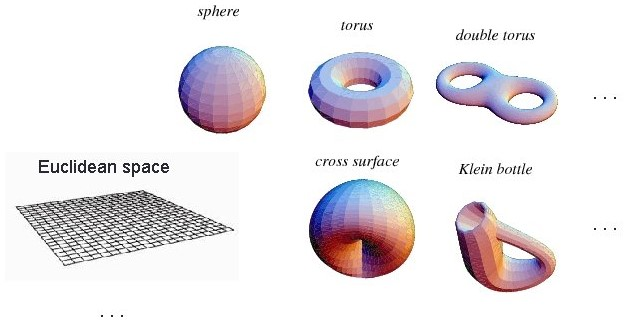
\includegraphics[width=0.4\textwidth]{figures/intro/manifold.jpg}
     \caption{Examples of $2$-dimensional manifolds.}
    \end{figure} 
            
Formally, the neural manifold is a lower-dimensional topological space embedded in the high-dimensional Euclidean space where the original neural output belongs. Why is the neural manifold still a good representation of the organization of neurons even if it is of a lower dimension?  The general justification rests on ``the Manifold Hypothesis\footnote{the Manifold Hypothesis forms the basis of a collection of methods called Manifold Learning}," which states that naturally occurring data form lower-dimensional manifolds in the embedding space \cite{colah-manifold}. The neuroscientific justification is based on the established fact that despite the original high-dimensional representations, the possible patterns of neural output are confined to a lower-dimensional manifold spanned by a few independent patterns called ``neural modes"  \cite{gallego_neural_2017}, \cite{stopfer_intensity_2003}, \cite{yu_gaussian-process_2009}.

% In other words, the number of variables that are really necessary to describe the data is much smaller than the number of variables in the original representation.
\begin{rmk}
For ease of reference, we also use the term ``neural manifold" for the point-cloud of data points with an underlying manifold structure. In addition, neural manifolds from real neural data are often no longer ``manifolds” in a mathematical sense, due to the sparse input sampling and the presence of neural noise. 
\end{rmk}

\subsection{\textit{What can we analyze from a neural manifold?}}
\label{intro-network-manifold}
Neural manifold is an intermediate step from the neural output towards inferring the neural circuits. On the neural manifold, each point represents a neuron. The distance between a pair of points indicates how similar the firing patterns of the corresponding neurons are, and equivalently, how likely they participate in the same neural circuit. To infer the (unknown) neural circuit from a neural manifold (known), we note that there are three possible cases: if neurons were originally sampled 
\begin{enumerate}[noitemsep,topsep=0pt]
    \item from a collection of isolated neural circuits (decomposable networks), then the neurons would have distinct stimuli preferences, yielding a discontinuous neural manifold.
    \item from overlapping neural circuits (partially decomposable networks), most neurons would respond to multiple stimuli, leading to a smooth transition in stimuli preferences and a continuous neural manifold. 
    \item from fully connected neural circuits (non-decomposable networks),  all neurons would respond to all stimuli, and there would be no stimuli preferences across groups of neurons. This would yield a zero-dimensional (i.e., degenerate) manifold.
\end{enumerate}

\begin{figure}[H]
\label{networks-manifolds}
\centering
    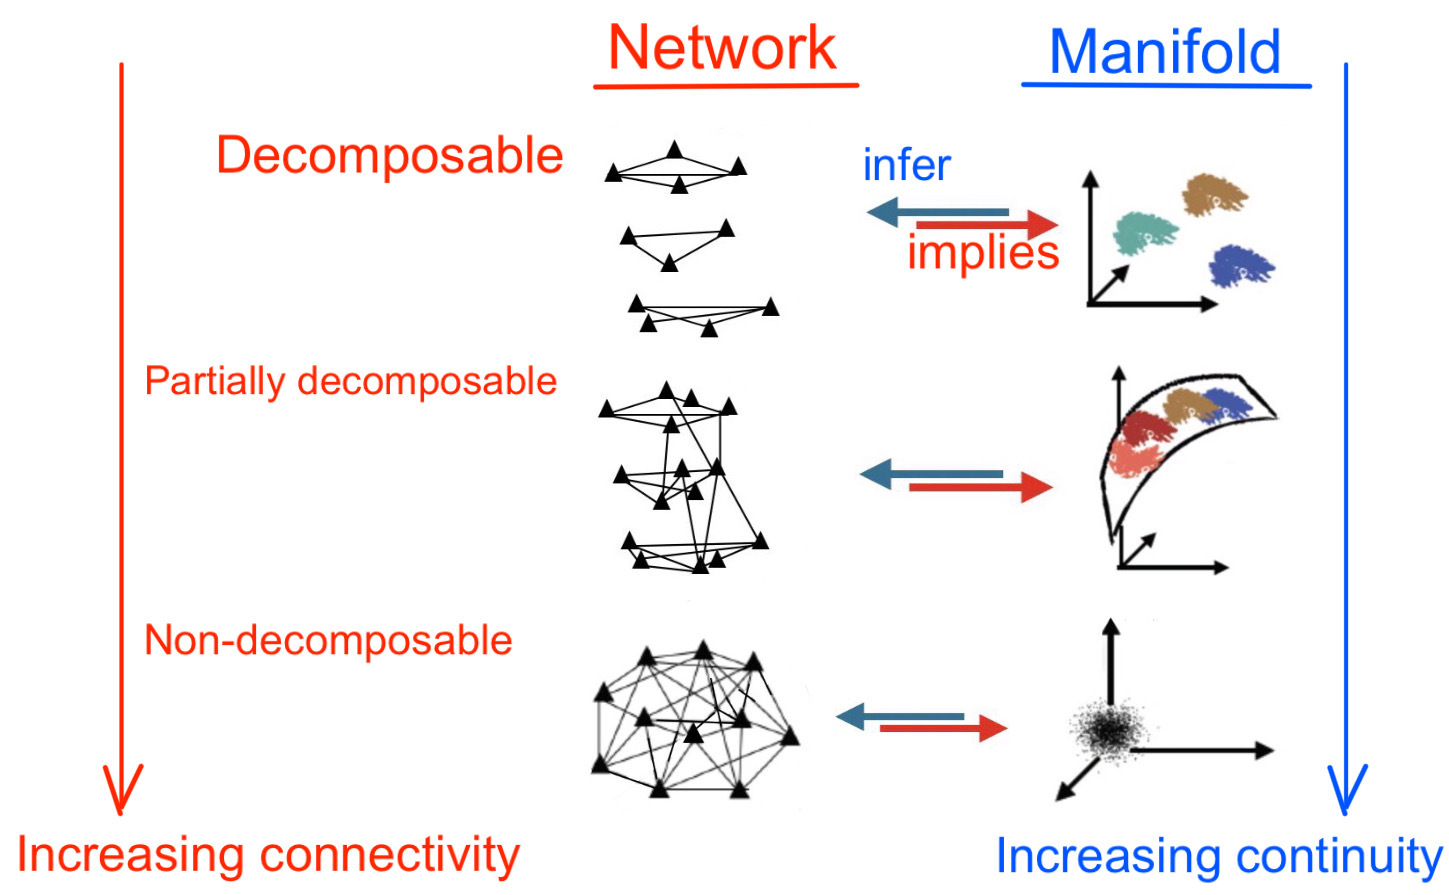
\includegraphics[width=0.55\textwidth]{figures/intro/networks-manifolds.jpg}
    \caption{Connections between neural manifolds and neural circuits. Adapted from \cite{dyballa_manifold_2021}.}
\end{figure} 
To sum up, by comparing the continuity of neural manifolds arising from artificial and biological neural networks, we can make precise inferences about their similarities and differences of their respective neural circuits, which is what we set out to compare in \ref{intro-motivation}.


\section{Problem statement}
\label{intro-objective}

Our starting point was the result in \cite{dyballa_manifold_2021}: based on the respective neural manifolds, the retinal ganglion cells differ fundamentally from the functional cells in V1 which are distributed more continuously. 
% \begin{figure}[H]
% \centering
% \begin{subfigure}[b]{0.5\textwidth}
%             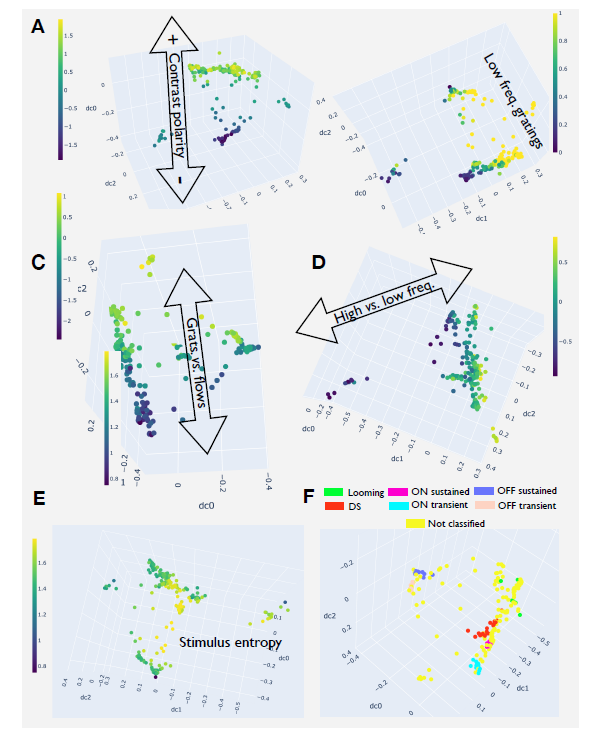
\includegraphics[width=0.6\textwidth]{figures/embeddings/retina-manifold.PNG}
%             \caption{Retina neural manifold (discontinuous).}
% \end{subfigure}
% \hfill
% \begin{subfigure}[b]{0.4\textwidth}  
%       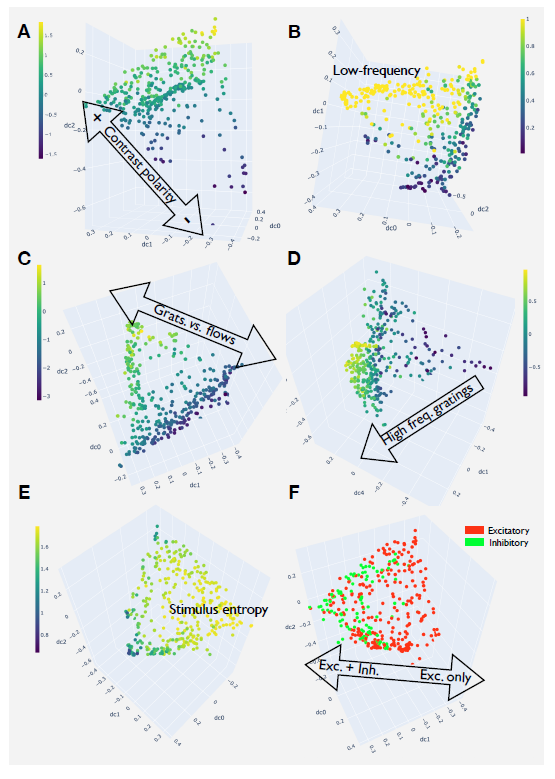
\includegraphics[width=0.6\textwidth]{figures/embeddings/v1-manifold.PNG}
%       \caption{V1 neural manifold (continuous).}
% \end{subfigure}

% \end{figure}     

Therefore, our objective, stated in concrete terms, is to find out among the computer vision models, which yield continuous neural manifold like V1 and which yield discontinuous neural manifold like the retina. The candidate models are CNN, Vision Transformer (ViT), and Recurrent Neural Networks (RNN), and their respective input and output are summarized in the following table.

\begin{table}[H]
\centering
\begin{tabular}{|l|l|l|}
\hline
        & Biological & Artificial     \\ \hline
Models   & retina, V1      & CNN, ViT, RNN \\\hline
Input & flow stimuli \cite{visual-flow}  & ImageNet images \cite{deng2009imagenet} \\ \hline
Output & single-neuron recording & artificial neuron output \\ \hline
\end{tabular}
\caption{Summary of comparison.} 
\end{table} 

% Building on our starting point, we obtained some original results, which can be summarized in the following conjectures to be further tested and confirmed:

% \textbf{Conjecture 1.} The manifold structure in feed-forward networks, including CNN and ViT, give rise to discontinuous neural manifold that is closer to that in retina than that in V1.

% \textbf{Conjecture 2.} Adding recurrent structure to the networks makes the manifold structure more continuous.

% justifications for doing comparison this way:
% why comparing with computer vision models?
% why choose continuity of manifold as the basis for comparison
% a good proxy for what kind of computation give rise to a continuous manifold

% basis of comparison: continuity of manifold this shows us the functional connections

% the models: CNN (convolution), RNN (recurrence), ViT (self-attention)

% By comparing the manifold structures of biological and artificial neural networks we can make precise inferences about similarities and differences in their respective functional circuits.

% conclusion: not convolution, not self-attention, but recurrence
\section{Highlights and thesis organization}

During the project, we have made the following original contributions:
\begin{enumerate}[noitemsep, topsep=0pt]
    \item conducted new computational experiments on neural data in the retina,
    \item developed an original algorithm to investigate the manifold structure of pre-trained Convolutional Neural Network (CNN) and how it evolves over the course of training,
    \item developed an original algorithm to investigate the manifold structure of pre-trained Convolutional Recurrent Neural Network (CRNN),
    \item developed an original algorithm to investigate the manifold structure of pre-trained Vision Transformer (ViT),
    \item compared and analyzed (both qualitatively and quantitatively) the manifold structure of CNN, ViT, and CRNN, against that of the neurobiological networks in retina and V1,
    \item conclusion that could advance research in both biological vision and computer vision.
\end{enumerate}

The code for this project is available at the GitHub repository\footnote{https://github.com/zhang-liu-official/capstone-liu-2022}.


The organization of the thesis follows the structure of the project in the flowchart below. After situating our work within the backdrop of related research in Chapter \ref{chapter-neuro}, we will provide the theoretical preliminaries for the linear dimensionality reduction method in Chapter \ref{chapter-linear} (its nonlinear counterpart is outlined in Appendix \ref{appendix-diffmap}). The experiments and results for biological and artificial neural networks will be elaborated in Chapters \ref{chapter-biological} and \ref{chapter-artificial} respectively. In the end, we propose the conclusion of our work and future directions. 


\vspace*{0.4cm}

\noindent\resizebox{\textwidth}{!}{\begin{tikzpicture}[font={\sf \small}]
 \def\smbwd{2cm}
  \node (BNN) at (-3.6,0.2) [draw, terminal, minimum width=\smbwd,  fill=yellow!20, minimum height=0.5cm] {Biological neural networks}; 
  \node (ANN) at (3.5,0.2) [draw, terminal, minimum width=\smbwd,  fill=yellow!20, minimum height=0.5cm] {Artificial neural networks}; 
  %------------
  \node (experimental) at (-3.6,-0.8) [draw, terminal, minimum width=\smbwd,  fill=red!20, minimum height=0.5cm]{Neural tensor (lab)};
  \node (artificial) at (3.5,-0.8)[draw, terminal,minimum width=\smbwd,  fill=red!20, minimum height=0.5cm]{Neural tensor (simulations)};
  %------------
  \node (TCA) at (0,-2)  [draw, process, minimum width=\smbwd, fill=blue!20, minimum height=0.7cm] {Dimensionality reduction (linear [Chapter \ref{chapter-linear}]; nonlinear [Appendix \ref{appendix-diffmap}])};
  %------------
  \node (biological-manifolds) at (-3.7,-3.2) [draw, terminal, minimum width=\smbwd,  fill=green!20, minimum height=0.5cm] {Neural manifold (biological) [Chapter \ref{chapter-biological}]};
  \node (artificial-manifolds) at (3.7,-3.2) [draw, terminal, minimum width=\smbwd,  fill=green!20, minimum height=0.5cm] {Neural manifold (artificial) [Chapter \ref{chapter-artificial}]};
  %------------
 \path [line](BNN) -- (experimental);
 \path [line](ANN) -- (artificial);
 \path [line](experimental) -- (TCA);
  \path [line](artificial) -- (TCA);
 \path [line](TCA) -- (biological-manifolds);
 \path [line](TCA) -- (artificial-manifolds);
 \end{tikzpicture}}

\chapter{Related works} 
\label{chapter-neuro} 
\section{Modeling biological vision}

\subsection{Hierarchy Models}
\par Hubel and Wiesel's hierarchy model \cite{hubel_receptive_1962} was the first seminal work on modeling the visual system, which classified the neurons in the primary visual cortex (V1) into simple and complex cells. The essential difference between simple and complex cells is that the responses of simple cells are modulated by the spatial phase of a sine grating, whereas the responses of complex cells are largely phase invariant. In other words, as we progress from simple cells to complex cells, the neurons become selective for increasingly complex stimuli and become more tolerant to the exact position within their receptive fields. Based on this, a natural way to construct complex cells is to group responses from simple cells that have the same orientation preference but different phase preferences.

\par This idea directly inspired the Neocognitron model \cite{fukushima_neocognitron_1980}. In the Neocognitron model, simple cells (termed as ``S-cells" in the original paper) are tuned to simple stimuli at the convolution layers. Their outputs are then combined at the pooling layers by taking the maximum or average to form complex cells (termed as ``C-cells" in the original paper). As a result, complex cells are tuned to more complex stimuli. The Neocognitron model was among a myriad of hierarchical models of the visual system and inspired the structure of CNN.

\par The figure below shows a systematic illustration of the general idea behind the hierarchical models:
\begin{figure}[H]
\centering
    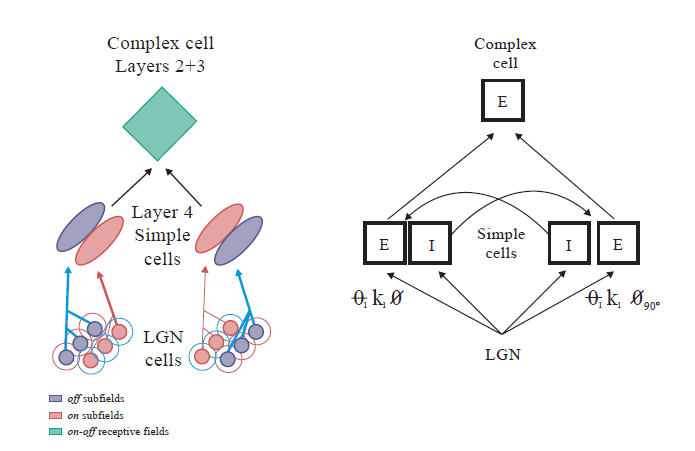
\includegraphics[width=10cm]{figures/models/hierarchical-models.png}
     \caption{Illustration of the hierarchical models \cite{martinez_complex_2003}.}
\end{figure}

\par Hierarchical models have several advantages :
\begin{itemize}
    \item If a visual recognition task can be decomposed into low-complexity learning tasks through the layers, then each layer would need only a small set of training data \cite{poggio2003mathematics}.
    \item The lower levels of the hierarchy might represent a dictionary of features that can be shared across various classification tasks \cite{geman1999hierarchy}, thus increasing efficiency.
\end{itemize}

\par There are also some known limitations of hierarchical models:
\begin{itemize}
    \item Hierarchical models assume that the computations at each successive stage being largely feed-forward \cite{riesenhuber1999hierarchical}, \cite{dicarlo2012does}. This is limited because back-projections are also likely to be a key part of the visual system. 
    \item The anatomical hierarchy should be considered an idealization instead of a strict flowchart of visual information \cite{hegde2007reappraising}. 
    % \par One particularly interesting piece of evidence: a close comparison of shape representation between V1, V2 and V4 also demonstrated a complex pattern of shape selectivity with significant deviation from strict hierarchical organization with some cells in V1 exhibiting more complex tuning than some cells in V4 (\cite{hegde2007reappraising}).
\end{itemize}

\subsection{Recurrent Models}
\label{neuro-recurrent}
\par Increasingly, recent experimental and computational evidence has suggested  alternatives to the hierarchical model, notably recurrent models \cite{martinez_complex_2003}.

% \begin{itemize}
% \item \textbf{Parallel Models:} The first strong evidence against the hierarchical model was the discovery that some complex cells, like simple cells, receive monosynaptic input from the thalamus \cite{hoffmann1972relay}. Based on this discovery, Hoffman and Stone proposed that both cell types, simple and complex, were generated in parallel by separate thalamocortical pathways, as shown in diagram A in Figure \ref{fig:parallel-models}. 
% \begin{figure}[H]
% \centering
%     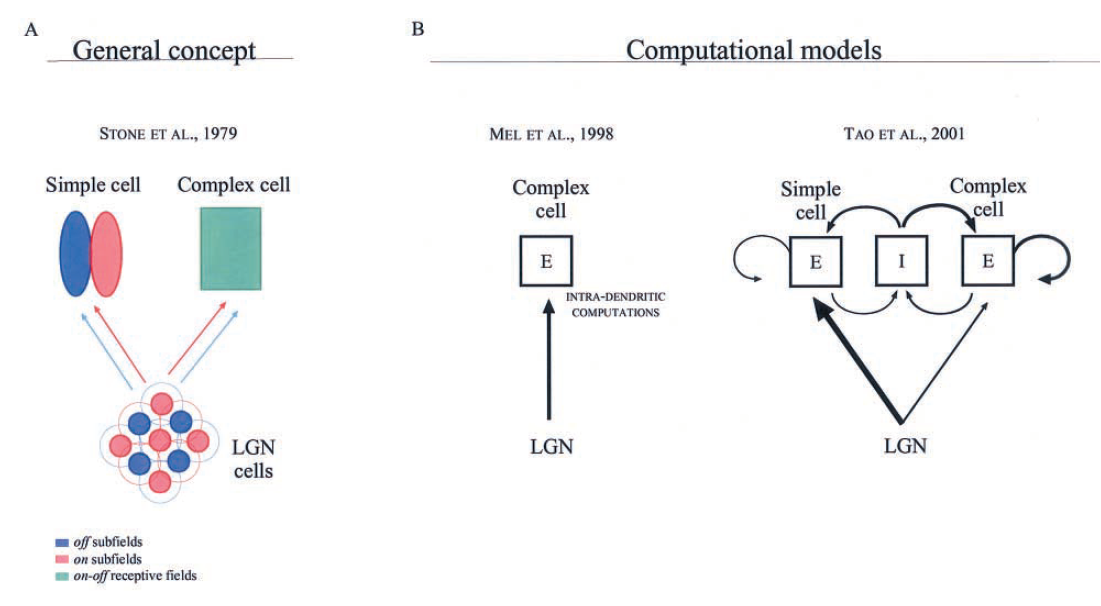
\includegraphics[width=10cm]{figures/models/parallel-models.png}
%      \caption{Illustration of the parallel models \cite{martinez_complex_2003}}
%      \label{fig:parallel-models}
% \end{figure}

% \par Simple cells and complex cells are far from being two parallel cortical pathways in the same way that X and Y cells are parallel thalamic pathways. However, the idea that some complex receptive fields can be generated at
% least in part by direct thalamic inputs is likely to be correct \cite{martinez_complex_2003}.

\par Recurrent models changed the focus of attention from single cells to networks of cortical connections \cite{martinez_complex_2003}. An illustration for recurrent models are shown in Figure \ref{fig:recurrent-models}.

\begin{figure}[H]
\centering
    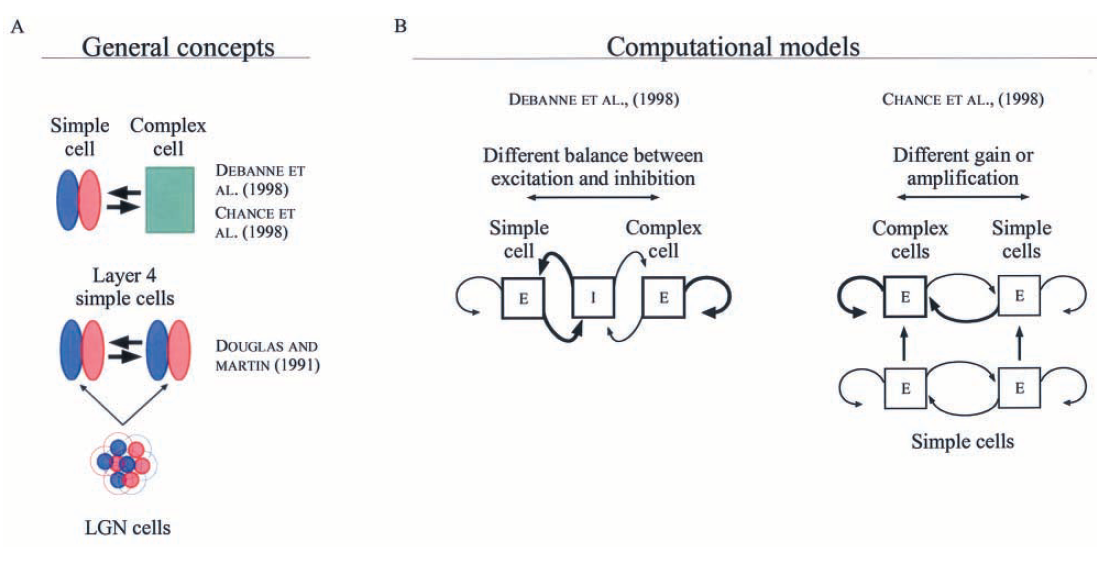
\includegraphics[width=10cm]{figures/models/recurrent-models.png}
     \caption{Illustration of the recurrent models \cite{martinez_complex_2003}.}
     \label{fig:recurrent-models}
\end{figure}

In addition, more recently, recurrent models of the visual system has inspired a new topic of research that focus on applying the idea behind recurrence model to show and/or address limitations of computer vision models. Among other similar works (\cite{oreilly_recurrent_2013}, \cite{spoerer_recurrent_2017},  \cite{kietzmann_recurrence_2019}, \cite{van_bergen_going_2020}), two notable recent works are \cite{ricci_same-different_2018}, which proposed that feedback mechanisms including attention and perceptual grouping are key to visual relational reasoning tasks and \cite{kietzmann_recurrence_2019}, which showed that recurrence is necessary to model the representational dynamics in the visual system.

% [to-do: expand on this further if there is time]

Till today, there are still many debates over which models best capture the neural circuits in the visual system and whether and how computer vision models can incorporate certain features of biological vision. Our work builds on the above existing line of research and provides some original insights to open questions that are relevant to these debates. 


\section{Neural manifold theory}
Throughout the historical progress in neuroscience, there have been numerous efforts to apply geometric and topological methods from related fields in mathematics and computer science, including computational geometry, differential geometry, spectral graph theory, and algebraic topology, among many others. Recently, studying the structure of neural population response with high-dimensional neural spiking data has become a commonly used technique in studying the structure of brain cortices. The high-dimensional nature of neural spiking data have thus motivated various linear and non-linear dimensionality reduction methods. 

In \cite{chung_neural_2021}, neural manifold is defined as a set of geometric structures in neural population activity underlying different cognitive tasks. 
% provided a comprehensive review of the recent studies that have applied geometric and topological methods to discover the properties of neural population geometry. 
% \cite{chung_classification_2018} proposed the ``object manifold" which

The authors of \cite{gallego_neural_2017} were the first to propose the concept of ``neural modes," which are specific patterns of correlated neural activity that span the neural manifolds. They thus proposed a generative model of individual neuronal activity based on the activation of neural modes. The parameters of such model can be obtained using dimensionality reduction methods. \cite{williams_unsupervised_2018} used linear dimensionality reduction method of tensor CANDECOMP/PARAFAC (CP) decomposition to discover low-dimensional neural dynamics by extracting three ``tensor factors," which are interconnected, low-dimensional descriptions of neural data.

% \section{Brain-inspired Computer Vision}
% \label{brain-inspired}
% [to-do]
\chapter{Dimensionality Reduction} 
\label{chapter-linear} 

As explained in section \ref{intro-framework}, our basis for comparison is the neural manifold, which is a lower-dimensional representation of the original neural output. This requires the use of an appropriate dimensionality reduction method\footnote{Linear dimensionality reduction methods work well when the data lie near a linear subspace of high-dimensional space. They suffice for the purpose of the project thus far, but when the data lie near a nonlinear manifold , a nonlinear dimensionality reduction method might be more suitable \cite{fefferman_testing_2016}. Therefore, we also introduce the nonlinear dimensionality reduction technique of diffusion map in Appendix \ref{appendix-diffmap}.}. In this thesis, we focus on the linear dimensionality reduction method, tensor CANDECOMP/PARAFAC (CP) decomposition, a higher-order generalization of Principal Component Analysis (PCA)\footnote{In this chapter we assume familiarity with PCA, but interested reader could refer to Appendix \ref{appendix-pca} for notes on PCA.}. This higher-order generalization is necessary because the neural output has three dimensions, namely neurons, stimuli, and time steps (which will be further explained in Chapter \ref{chapter-biological}). 

\section{Tensor CP decomposition}
\begin{defn}[Tensor]
    An $N$-way \underline{tensor} is defined as an element of the tensor product of $N$ vector spaces. A $1$-way tensor is a vector. A $2$-way tensor is a matrix.
    \end{defn}

\begin{defn}[Tensor norm]
The \underline{norm of tensor} $\mathcal{X} \in \RR^{I_1 \times I_2\times\cdots I_N}$ is
\begin{align}
    \norm{\mathcal{X}} = \sqrt{\sum_{i_1 = 1}^{I_1}\sum_{i_2 = 1}^{I_2}\cdots \sum_{i_N = 1}^{I_N} x_{i_1 i_2 \dots i_N}^2 }.
\end{align}
\end{defn}
\begin{defn}[Rank-one tensor]
An $N$-way tensor $\mathcal{X} \in \RR^{I_1 \times I_2\times\cdots I_N}$ is \underline{rank-one} if it can be written as the outer product of $N$ vectors, that is,
\begin{align}
    \mathcal{X} = \aaa^{(1)}\circ \aaa^{(2)} \circ \cdots \circ \aaa^{(N)}
\end{align}
\end{defn}

Analogous to PCA, tensor CP decomposition aims to approximate the original tensor by a sum of rank-one tensors, each of which can then be written as the outer product of $N$ vectors. Given a $3$-way tensor $\mathcal{X} \in \RR^{I\times J\times K}$, the tensor CP decomposition model is formulated as
\begin{align}
    \mathcal{X} \approx [\![ \mathbf{A}, \mathbf{B}, \mathbf{C} ]\!] = \sum_{r=1}^R \aaa_r \circ \bbb_r \circ \ccc_r,
\end{align}
where $R$ is the rank of the tensor, i.e., the minimal number of rank-1 tensors necessary to represent the tensor. $a_r \in \RR^I, b_r \in \RR^J, c_r \in \RR^K$ for $r = 1,\dots, R.$ Determining the rank $R$ of a specific given tensor is difficult; in fact, the problem is NP-hard. Thus, typically the goal is to find the low-rank approximation of the true rank, i.e., $R$ as an approximation of the true rank $M$ and $R < M$.

% The element-wise formulation analogous to \ref{pca} is 
% \begin{align}
%     x_{i j k} \approx \sum_{r=1}^R a_{i r} b_{j r} c_{k r}
% \end{align}
% for $i = 1,\dots, I, j = 1,\dots, J, k = 1,\dots,K.$

With tensor CP decomposition, we obtain the tensor factors which are analogous to the principle components in PCA. These neural factors can then be used as lower-dimensional representation of the tensor data. This can be illustrated with the diagram below. These neural factors can be used as lower-dimensional representation of the tensor data.
\begin{figure}[H]
    \centering
        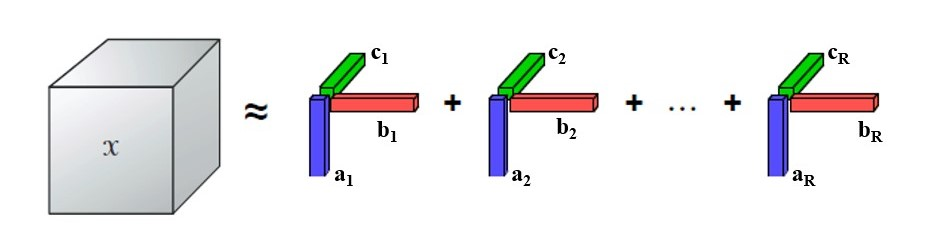
\includegraphics[width=0.7\textwidth]{figures/linear/tca.jpg}
        \caption{Illustration for tensor CP decomposition. (Adapted from \cite{williams_unsupervised_2018})}
    \end{figure} 

% The alternating least squares (ALS) method in \cite{kolda_tensor_2009} is one of the most common algorithms to compute a tensor CP decomposition with $R$ components. The steps of the ALS are summarized as follows: 
% \begin{enumerate}
%     \item fix  $\mathbf{B}$ and  $\mathbf{C}$ to solve for $\mathbf{A}$: 
%      \begin{equation}
%       \min_{\mathbf{A}} \sum_{i j k}\left(x_{i j k} - \sum_l a_{i l} b_{j l} c_{k l}\right)^2
%      \end{equation}
%     \item fix $\mathbf{A}$ and  $\mathbf{C}$ to solve for  $\mathbf{B}$:
%   \begin{align}
%       \min_{\mathbf{B}} \sum_{i j k}\left(x_{i j k} - \sum_l a_{i l}  b_{j l} c_{k l}\right)^2
%      \end{align}
%  \item fix $\mathbf{A}$ and  $\mathbf{B}$ to solve for $\mathbf{C}$: 
%  \begin{align}
%       \min_{\mathbf{C}} \sum_{i j k}\left(x_{i j k} - \sum_l a_{i l}  b_{j l} c_{k l}\right)^2
%      \end{align}
% \end{enumerate} 
% and repeat the above steps until some convergence criterion is satisfied. 

In selecting the optimization algorithm, we experimented with different optimization methods using the the generalized CP decomposition framework described in \cite{hong_generalized_2020}. In the end, gradient-based direct optimization approach (OPT) \cite{direct-opt}  was shown to give higher accuracy when the number of factors chosen is larger than the true rank (``overfactoring”). This could help inform us the number of factors to choose. 

Additionally, when the data has a non-negative constraint, Non-negative Tensor Factorization (NTF) is used. In NTF,
by adding the non-negative constraint, the original optimaization problem becomes:

 \begin{mini}|l|
  {\mathbf{A},\mathbf{B},\mathbf{C}}{\|\mathcal{X}- [\![ \mathbf{A}, \mathbf{B}, \mathbf{C} ]\!] \|_F^2}{}{}
  \addConstraint{\mathbf{A}, \mathbf{B}, \mathbf{C} \geq 0.}
 \end{mini}
Henceforth we will refer to the chosen linear dimensionality reduction method (tensor CP decomposition using direct optimization with non-negative constraint) as Non-negative Tensor Factorization (NTF).



\chapter{Biological Neural Networks} 
\label{chapter-biological} 

In this chapter, we describe our experiments to test and extend the findings in \cite{dyballa_manifold_2021} on a different  data set collected from the retina.

\section{Neural tensor for retina}
The neural spiking data \cite{dyballa_manifold_2021} were collected from lab experiments with the setup shown in the figure below. Six different types of flow stimuli developed in \cite{visual-flow} were flashed in front of the mouse. The electrodes recorded the neural output from the mouse's retina while it viewed each flow stimuli moving in eight directions respectively. The neural recordings were encoded in peristimulus (PSTH) diagrams, each of which showed the firing rate of one neuron over time for the eight directions respectively. In the PSTH diagram the brighter pixels indicate higher firing rates.
\begin{figure}[H]
    \centering
        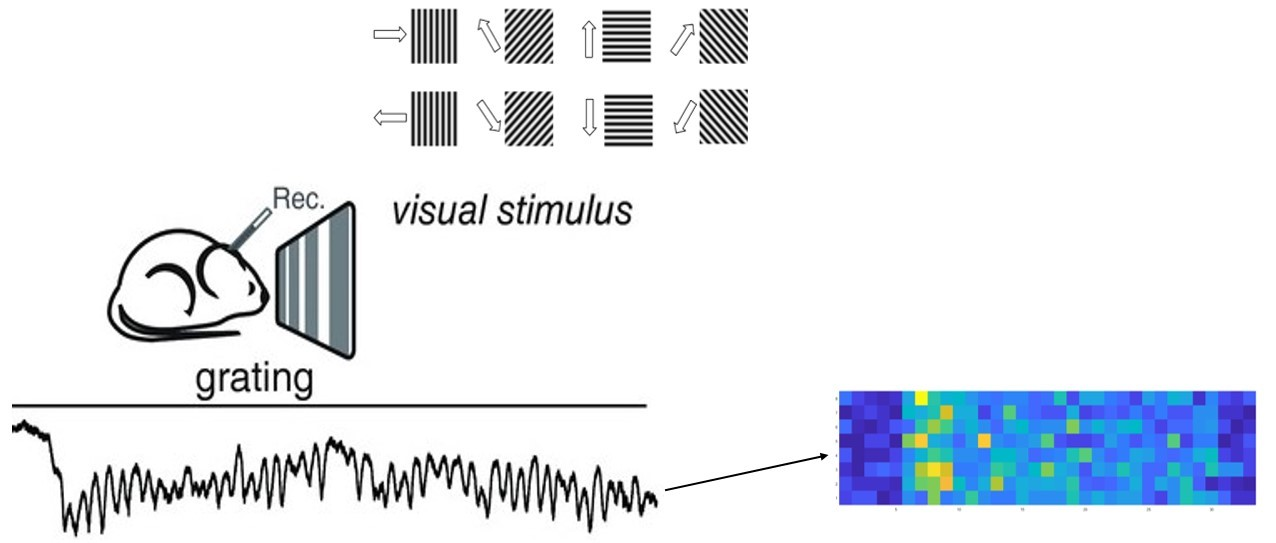
\includegraphics[width=0.6\textwidth]{figures/biological/biological-input-output.jpg}
        \caption{Visualising neural data from lab experiments.}
\end{figure}

\par The neural spiking data is of three dimensions: the first dimension represents the $698$ neurons; the second dimension represents the six different types of stimuli; the third dimension represents the vectorized PSTH diagrams, each of which has $8\times 33 = 264$ pixels. This gives us a $3$-way tensor:

\begin{defn}[Neural tensors]
    Suppose $\mathcal{S}$ is a set of flow stimuli $\mathcal{S} = \{s_1, s_2,\dots, s_K\}$, each moving over  $T$ time steps. The \underline{neural population response} of a set of $N$ neurons to some stimulus $s_i$ over time is $\mathcal{N} = \{\vec{n}_1, \vec{n}_2, \dots, \vec{n}_N\},$ where $\vec{n}_i \in \mathbb{R}^{T}$. 

    Each \underline{neural tensor} encodes the neural population response of $N$ neurons to $K$ flow stimuli over $T$ time steps and is thus a $3$-way $N$-by-$K$-by-$T$ tensor.
\end{defn}

\section{Neural factors for retina}
We implement the Non-negative Tensor Factorization (NTF) using the Tensor Toolbox for MATLAB \cite{tensortoolbox}. Our algorithm is as follows:

\setcounter{algocf}{1}
\begin{algorithm}[H]
\setstretch{1}
\caption{Algorithm for NTF on retina tensor.}\label{alg:factors-retina}
\KwData{Neural tensor for retina.}
\KwResult{$R$ tensor factors for retina.}
\DontPrintSemicolon
import data as X, X = tensor(X) \;
chosen rank, R = 35 \;
n\_repetitions = 10, initialize errors with zeros \; 
\For{r from 1 to R}{
\For{rep from 1 to n\_repetitions}{
NTF: M = cp\_opt(X, r, 'init', 'rand' , 'lower', 0) \;
error = norm(X - tensor(M)) / norm(X); \;
add error to the array of errors \;
}
}
F\_neuron = M.u\{1\}, F\_stimuli = M.u\{2\}, F\_time = M.u\{3\} \;
save the factors \;
\end{algorithm}

We plot the reconstruction error curves to compare the performance of tensor CP decomposition when different optimization methods are used. ALS with random initialization and regular direct optimization perform better than non-negative direct optimization. However, since the neural output from biological neural networks is always non-negative, in order to ensure the interpretability of the resulting tensor factors in the context of our application, we choose to use non-negative direct optimization despite its relatively worse performance (which is not a crucial concern in our application since the neural factors obtained in this process are still good enough approximation of the original neural data).

\begin{figure}[H]
\centering
    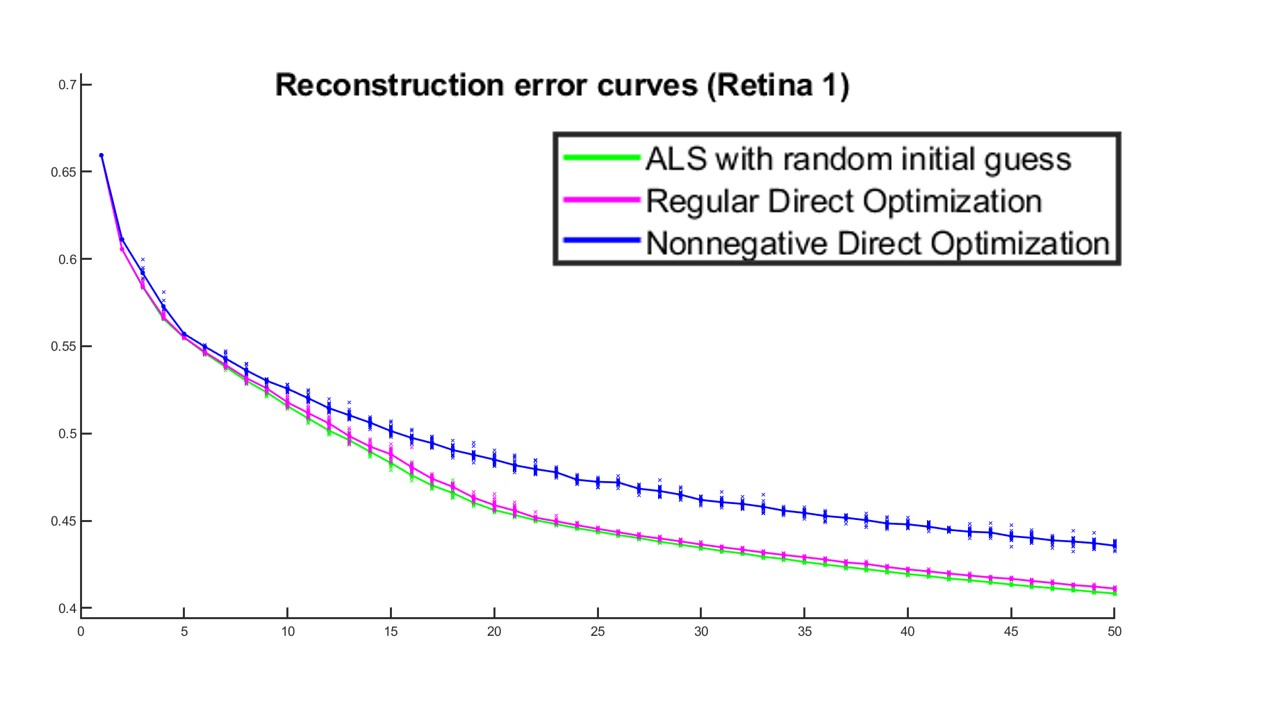
\includegraphics[width=0.6\textwidth]{figures/biological/retina1-reconstruction-error.jpg}
     \caption{Reconstruction errors of different optimization methods.}
\end{figure}  

We can visualize the resulting tensor factors:
\begin{figure}[H]
    \centering
        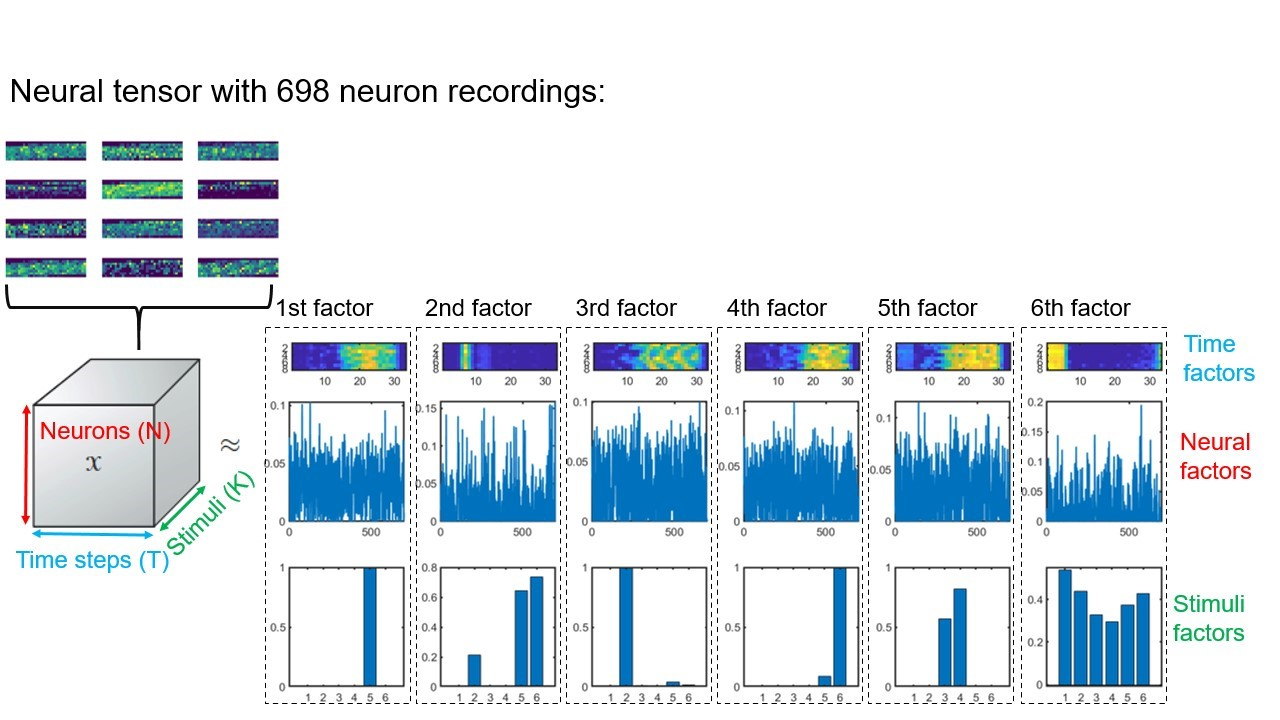
\includegraphics[width=0.8\textwidth]{figures/biological/retina-factors.jpg}
        \caption{First six tensor factors for retina.}
    \end{figure} 

\section{Neural manifold for retina}
The tensor factors form what we call the ``neural matrix" of dimension $(N,R)$, where $N$ is the number of neurons and $R$ is the chosen rank. Since the tensor factors provide an approximation of the original neural spiking data, we use PCA to project neural matrix onto a linear subspace with the same dimension, i.e., the number of components is $R$. We then use k-means clustering to label the clusters by distances in the lower-dimensional linear subspace. By choosing the optimal number of clusters to be six based on the experiments, we obtain the neural manifold for retina. In the following plot, each point represents a neuron. From the visualization below, the neural manifold for retina is discontinuous and the PSTH diagrams within each cluster are similar. This implies that neurons form disconnected clusters grouped by their firing patterns, implying that neurons have distinct stimuli preferences. By using the the connections between neural manifolds and neural circuits explained in \label{networks-manifolds}, we can already infer that the neural networks in retina are characterized by isolated neural circuits. We extend this result further by quantifying the degree of continuity in the next section.
  \begin{figure}[H]
        \centering
             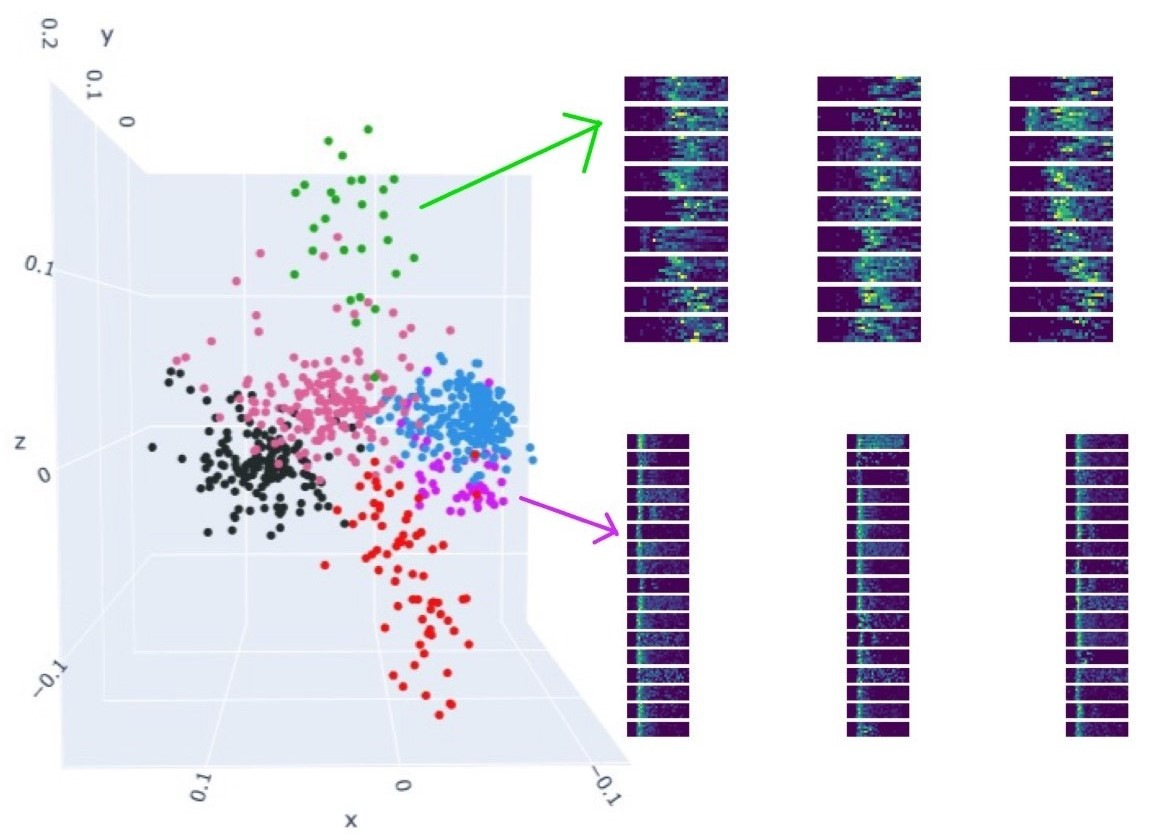
\includegraphics[width=0.7\textwidth]{figures/biological/retina-manifold-with-psth.jpg}
            \caption{Neural manifold for retina is discontinuous.}
        \end{figure} 

\subsection{Quantifying the continuity of the manifold}
Following the method proposed in \cite{dyballa_manifold_2021}, we compute the mean flow ratio (MFR) as a quantifiable measure to compare the continuity of the respective neural manifolds: the smaller the MFR, the more discontinuous the neural manifold is, and vice versa. The algorithm is outlined on the next page. The MFR of the retina neural manifold computed from our algorithm is $\phi_G = 0.56$. Now we compare the results with V1 using results from \cite{dyballa_manifold_2021}: the neural manifold for V1 is continuous in the visualizatoin below and the MFR of V1 is $\phi_G = 0.91$ as concluded in . The difference in the MFRs suggests that the neural manifold for V1 is much more continuous than retina. Thus, we can conclude that the neural circuit in V1 has much higher connectivity than retina. The results in this chapter will be used again in the next chapter to compare with results from the artificial neural networks.
 \begin{figure}[H]
        \centering
             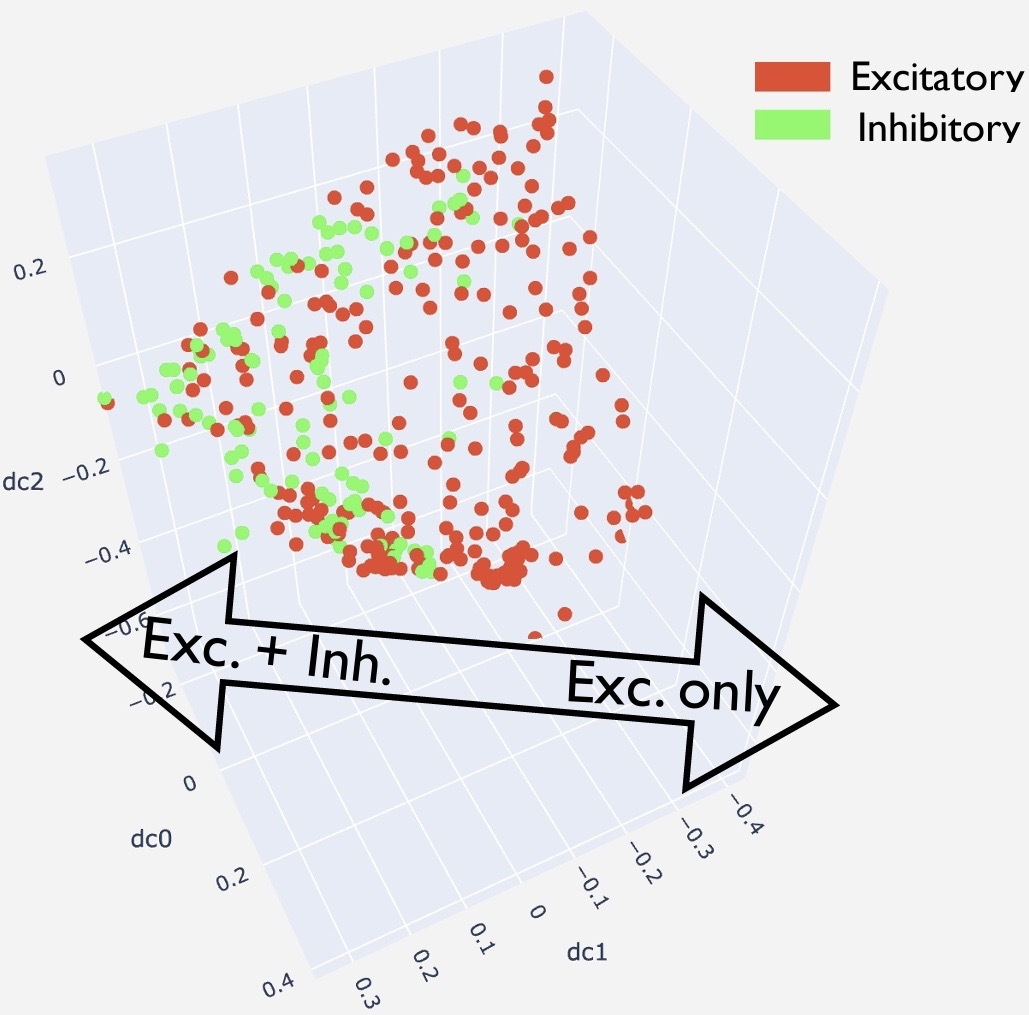
\includegraphics[width=0.45\textwidth]{figures/biological/v1-manifold.jpg}
            \caption{Neural manifold for V1 is continuous. The neurons are colored by excitatory and inhibitory functions and the two clusters overlap each other.}
        \end{figure} 
% The mean flow ratio has its origin in the maximum flow problem, a classic problem in graph theory originally formulated as a means to optimize railway traffic between cities \cite{schrijver_history_2002}.

\setcounter{algocf}{2}
\begin{algorithm}[H]
\setstretch{1}
\caption{Algorithm for computing the mean flow ratio.}\label{alg:mean-flow-ratio}
\DontPrintSemicolon
\KwData{points on the neural manifold, $\xx_1, \dots, \xx_N \in \mathcal{M}$.}
\KwResult{mean flow ratio for the neural manifold, $\phi_G$.}
kernel bandwidth, $\epsilon \coloneqq \frac{1}{N}\sum_{i=1}^N \min_{j: \xx_j \neq \xx_i}\|\xx_i - \xx_j\|^2$\;
Gaussian kernel\footnote{In fact, we can choose any symmetric, positive semi-definite similarity kernel. But Gaussian kernel gives a physically intuitive construction as it effectively considers a ball of radius $\epsilon$ around each data point.}, $k(\xx_i, \xx_j) = \exp(-\|\xx_i - \xx_j\|^2/\epsilon)$ \;
weight matrix $W, W_{i, j}\coloneqq {k_\epsilon}(\xx_i, \xx_j)$\;
degree of node $\xx_i$, $d(\xx_i) \coloneqq \sum_{j=1}^N W_{i,j}$\;
anisotropic Gaussian kernel, $\Tilde{k_\epsilon}(\xx_i, \xx_j) \coloneqq \frac{k_\epsilon(\xx_i, \xx_j)}{d(\xx_i)d(\xx_j)}$ \;
anisotropic weight matrix,$\Tilde{W}, \Tilde{W}_{i, j}\coloneqq \Tilde{k_\epsilon}(\xx_i, \xx_j)$\;
build graph $G = (V, E)$, weight of the edge ($\xx_i$, $\xx_j$) is $\Tilde{W}_{i, j}$ \;
edge resistance, $R_{i, j} = 1/\Tilde{W}_{i, j}$ \;
compute effective resistance $R^{\text{eff}}_{i, j}$, using \cite{effective-resistance}\;
effective conductance, $C^{\text{eff}}_{i, j} = 1/R^{\text{eff}}_{i, j}$\;
build graph $G_C$, weight of the edge ($\xx_i$, $\xx_j$) is $C^{\text{eff}}_{i, j}$  \;
\For{i from 1 to N}{
\For{j from 1 to N, $j\neq i$}{
SumAll += \text{maxflow}(i, j)\;
}
\For{k: k is a neighbor of i}{
SumNeighbors += \text{maxflow}(i, k)
}
flow ratio of node $\xx_i$, $\rho_i$ = SumAll/SumNeighbors\;
}
mean flow ratio of graph $G$, $\phi_G = \sum_{i=1}^N \rho_i.$
\end{algorithm}

\chapter{Artificial Neural Networks} 
\label{chapter-artificial} 

As we have established in the introduction, the key basis of comparison between artificial and biological neural networks is the continuity of the neural manifold. Qualitatively, we can make this comparison by visualizing both the tensor factors and the neural manifolds. Quantitatively, we can compare the mean flow ratio which provides a measure for how continuous the neural manifolds are. This chapter outlines our algorithms, key experiments, and findings for candidate models proposed in \ref{intro-framework}, which allow for a rigorous comparative analysis - these constitute our main contribution to the research literature. 

\section{CNN}
Our first candidate model is VGG16, one of the most successful CNN models in computer vision tasks such as image classification. Its architecture is shown in the figure below.
\begin{figure}[H]
    \centering
        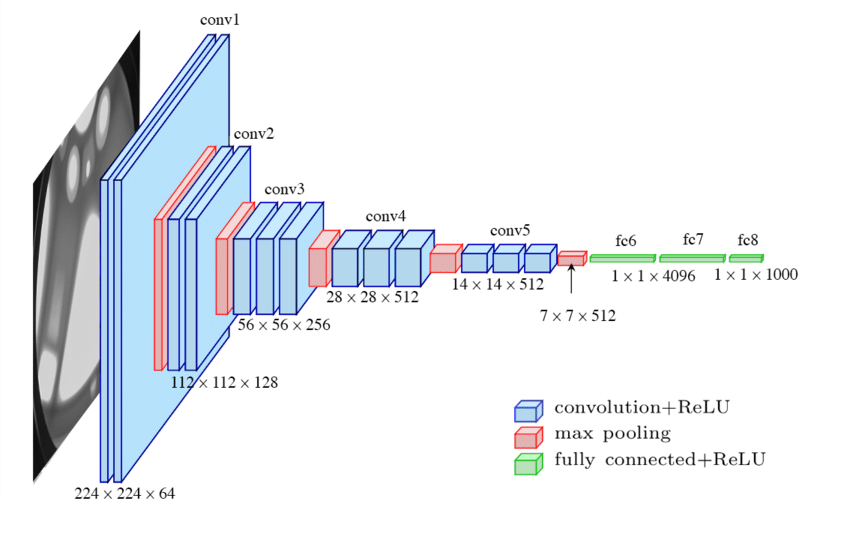
\includegraphics[width=0.5\textwidth]{figures/artificial/vgg16.png}
        \caption{Visualizing the structure of the VGG16 model.}
\end{figure}
    
\subsection{``Visual stimuli" in CNN}
Analogous to the flow stimuli in lab experiments, the ``visual stimuli" for CNN are natural images of different objects selected from the benchmark dataset ImageNet \cite{deng2009imagenet}. To keep the size of the artificial neural tensor manageable, we randomly selected 20 images from four classes as the visual stimuli. In order to simulate the movement of flow stimuli over time, we create multiple shifts of the original image in vertical and horizontal direction, with the shift step equal to the size of the filter. 
    % add image
    \begin{figure}[H]
        \centering
            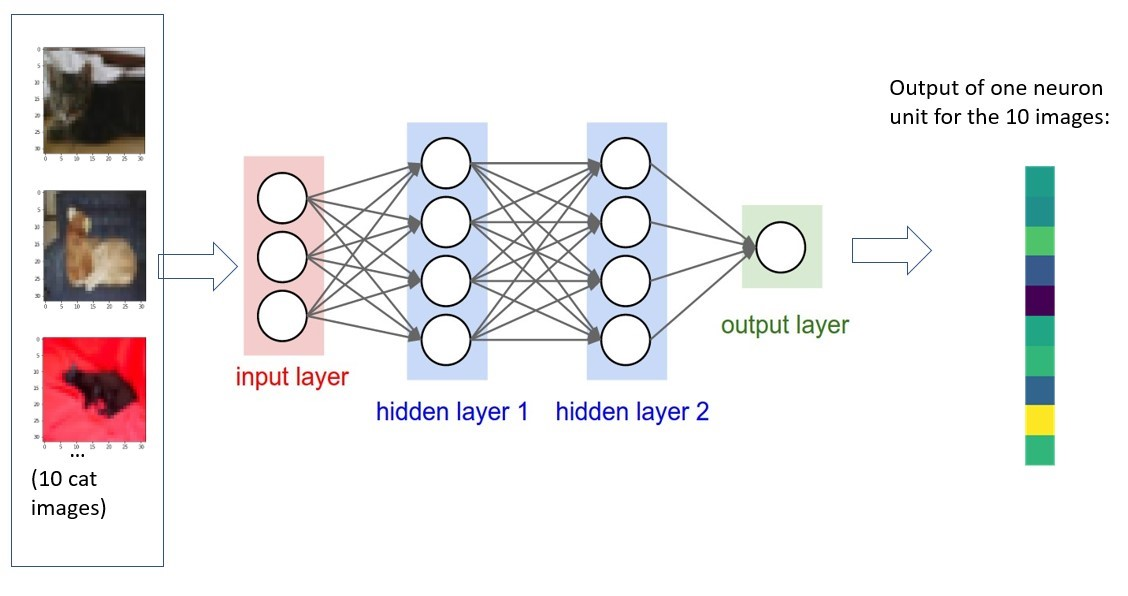
\includegraphics[width=0.7\textwidth]{figures/artificial/artificial-input-output.jpg}
            \caption{Computing output of one neuron unit in the CNNs given 10 input cat images.}
    \end{figure}
    
\begin{rmk}
At first it might seem that using different stimuli for biological and artificial neural networks will lead to an unfair comparison. However, this approach is appropriate for the following reason: The mouse visual system was trained on the flow stimuli is shown to resemble the naturalistic visual information that the mouse's vision has adapted to\footnote{Based on the paper that proposed flow stimuli \cite{visual-flow}, flow stimuli are more like what the mouse would encounter in the natural world than are sine-wave gratings but is more tractable for analysis than are natural images.}. The visual stimuli for VGG16 model came from the same data set that it is trained on (ImageNet). Thus, in both cases, the visual stimuli are similar to what the respective network was trained to recognize.
\end{rmk}
 
 \subsection{``Individual neuron" in CNN}
 In the lab experiments for biological neural networks, moving visual stimuli trigger spikes in the activation potential in the neurons in the retina. The individual neuron response is the firing rate of the neuron which is dependent on the  electrostatics processes that take place in the synapse. The biological neuron is coarsely modeled by the neuron unit in the CNNs. At the ``dendrite," the input is taken from the ``axons" of the connected neurons.\footnote{Note, however, that in our experiments, instead of taking the input from previously connected neuron unit, each neuron takes the image as the input.} The weight of each neuron models the synaptic process in biological neuron. At the ``cell body," all the inputs are multiplied with the weights and summed. We then add the bias term to the sum and apply the nonlinear activation to obtain the final output from the individual neuron unit at the ``axon." The parallel between biological and artificial neuron is shown in the figures below. 
\begin{figure}[H]
\centering
\begin{subfigure}[b]{0.5\textwidth}
        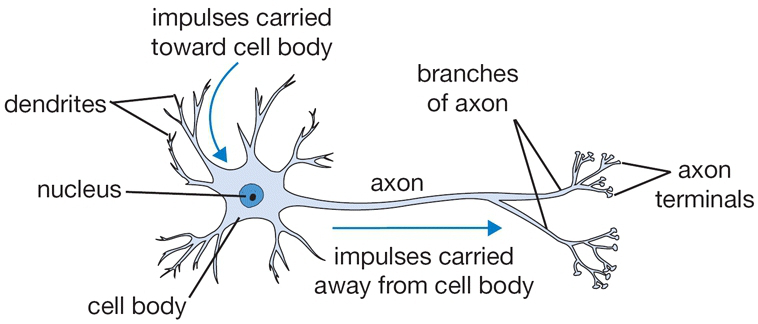
\includegraphics[width=0.9\textwidth]{figures/artificial/neuron.png}
        \caption{An individual neuron in biological neural networks. Adapted from \cite{cs231n}.}
\end{subfigure}
\hfill
\begin{subfigure}[b]{0.45\textwidth}
        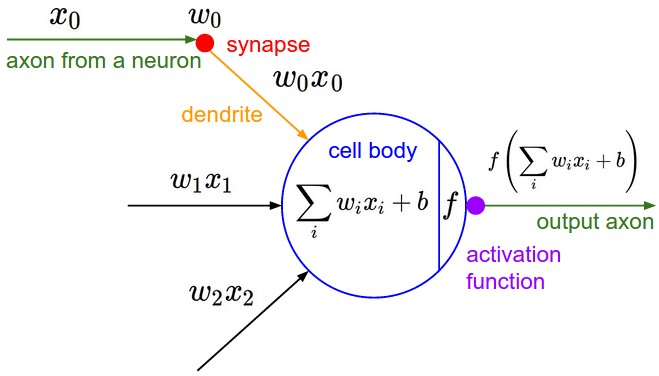
\includegraphics[width=0.9\textwidth]{figures/artificial/neuron_model.jpeg}
        \caption{An ``individual neuron" in CNNs. Adapted from \cite{cs231n}.}
\end{subfigure}
\end{figure} 

\subsection{``Receptive field" of an artificial neuron}
Each layer in the CNN has several different feature maps. Each feature map corresponds to a filter of a specific size and specific weights. The filter is essentially a matrix that, when taking inner product with the input image, give an output that highlights some specific features in the input image. To illustrate this, we can visualize the 64 feature map in the first convolutional layer of the VGG16 model, given the input image.
\begin{figure}[H]
\centering
\begin{subfigure}[b]{0.3\textwidth}
        \centering
  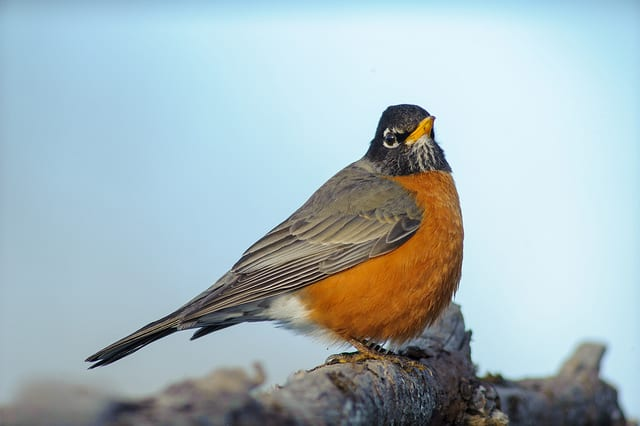
\includegraphics[width=0.6\textwidth]{figures/artificial/bird.jpg}
\caption{Input image. Adapted from \cite{feature_map}.}
\end{subfigure}
\hfill
\begin{subfigure}[b]{0.65\textwidth}
\centering
    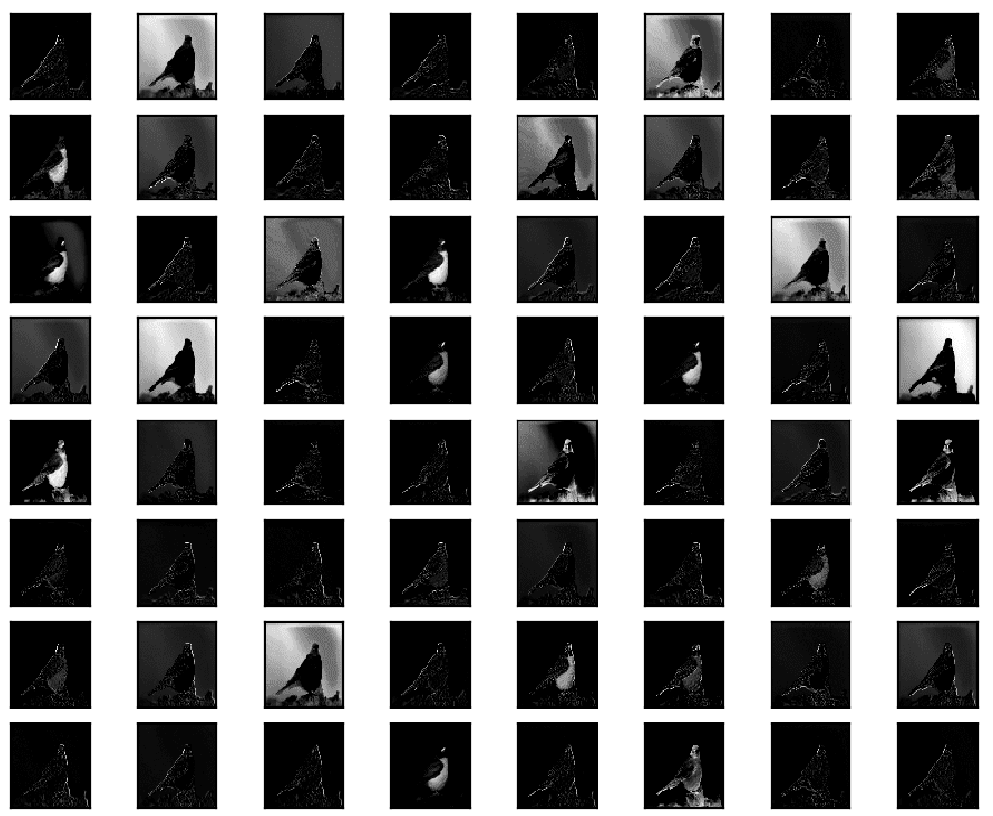
\includegraphics[width=0.45\textwidth]{figures/artificial/feature_map_vgg16.png}
    \caption{Visualizing the 64 feature maps in the first convolutional layer of the VGG16 model. Adapted from \cite{feature_map}.}
\end{subfigure}
\end{figure} 

The neurons within each feature map share the same weights and each attends to a specific subregion of the image which is referred to as their receptive field. This term originated from biological vision defined as a restricted region of visual space where a stimulus could illicit responses in a retinal ganglion cell. The size of the receptive field of a neuron is the same as the filter size corresponding to the feature map in which the neuron is located. 

 \subsection{``Neuron population response" in CNN}
Analogous to biological neural networks, we computed the neural output given the input image. Unlike biological neurons, most of the artificial neurons will have output of small values because most pre-trained weights decay to zero. In other words, the ``firing" of neurons in CNN will be sparse. We select the feature maps that contain the neurons with highest average firing rate.
% except for the specific neurons targeting at recognizing a specific features, 
% We now illustrate the dimensions of the resulting artificial neural tensor built from the first convolutional layer of VGG16. Since there were 1024 neurons in each feature map and we selected 10 feature maps, there were 10240 neurons in total. The visual stimuli consists of 10 images from each of the 10 classes, which give us 100 images. Each of the images have 1024 shifts. In the end, the size of the artificial tensor for the first convolutional layer is thus 10240-by-100-by-1024. 
\newpage
\setcounter{algocf}{1}
\begin{algorithm}[H]
\setstretch{1}
\caption{Algorithm for CNN artificial neural tensor.}\label{alg:cnn-tensor}
\DontPrintSemicolon
% Set Function Names
  \SetKwFunction{FShifts}{apply\_all\_shifts}
  \SetKwFunction{FOutput}{compute\_neuron\_output}
  \SetKwFunction{FStimuli}{show\_stimuli}
% Write Function with word ``Function''
  \SetKwProg{Fn}{Function}{:}{}
  \Fn{\FShifts{$image$, $shift\_step$}}{
        add the original image to image\_all\_shifts\;
        \For{i from 0 to \# vertical shifts}{
        shift the image vertically by shift\_step\;
        add the shifted image to image\_all\_shifts\;
            \For{j from 0 to \# horizontal shifts}{
            shift the image horizontally by shift\_step\;
            add the shifted image to image\_all\_shifts\;
            }
        }
  }
  \SetKwProg{Fn}{Function}{:}{}
  \Fn{\FOutput{$model$, $image\_all\_shifts$}}{
        \For{layer in all convolutional layers}{
        pass the image through the model\;
        take the neuron output from the specified layer after ReLU\;
        % , of shape (\# shifts, \# rows, \# columns, \# feature\_maps)\;
        % \# neurons in each feature map = \# rows * \# columns\;
        (optional) remove the neurons at the edges\;
        compute the average neuron output in each feature map\;
        select the feature maps with highest average \;
        normalize the neuron outputs in each feature map\;
        }
  }
  \SetKwProg{Fn}{Function}{:}{}
  \Fn{\FStimuli{$model$, $all\_images$}}{
        \For{image in images\_selected\_classes}{
        call \FShifts \;
        call \FOutput \;
        take average over outputs of all shifts of current image\;
        add to neuron\_output\_all\_images\;
        }
  }
\end{algorithm}

\subsection{Neural manifold for CNN}
In the plot below, each point in the data cloud represents a neuron. As shown by the disconnected clusters of neurons, the neural manifold for CNN is clearly discontinuous. When labeling the neurons according to their feature maps, we realize that these disconnected clusters are in fact organized by feature maps. This result aligns with the theoretical explanation that the neurons within the same feature map share the same filter weights. From shallow layer to deep layer, it is observed that although the clusters become more diffused, they were still form separate clusters with little overlap.

\begin{figure}[H]
\centering
\begin{subfigure}[b]{0.47\textwidth}
    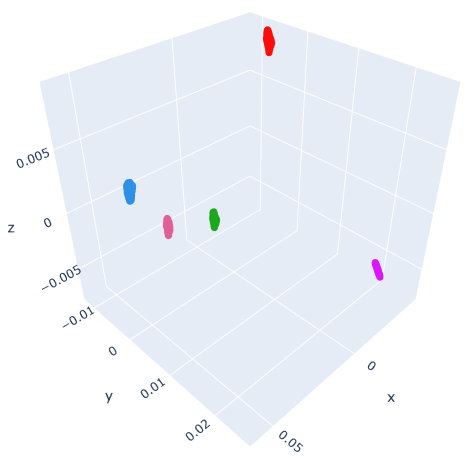
\includegraphics[width=\textwidth]{figures/embeddings/VGG16-2D-block1.png}
    \caption{VGG16 neural manifold (shallow layer).}
\end{subfigure}
\hfill
\begin{subfigure}[b]{0.45\textwidth}
    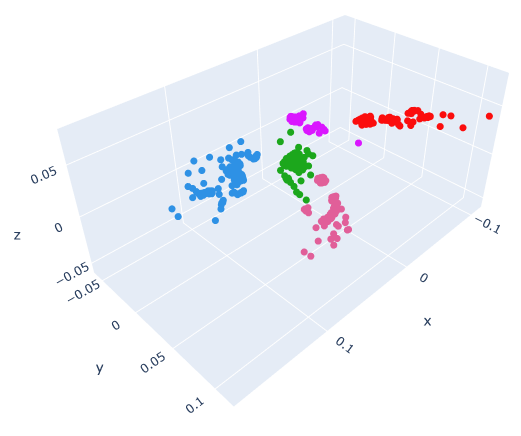
\includegraphics[width=\textwidth]{figures/embeddings/VGG16-2D-block3.png}
    \caption{VGG16 neural manifold (deep layer).}
\end{subfigure}
\end{figure}

In addition, by modifying line 24 in Algorithm \ref{alg:cnn-tensor} to appending the output for each shift instead of taking the average over all shifts, we obtain the neural manifold that preserves the spatial ordering of the neurons in the same feature map. The center and right plots below show the neurons within one cluster colored by their vertical and horizontal position. Since the neuron's coordinate on the neural manifold and the color aligns perfectly, this is good evidence that within a cluster, each neuron’s response corresponds to its spatial position given by the subregion it attends to.

\begin{figure}[H]
\centering
\begin{subfigure}[b]{0.37\textwidth}
    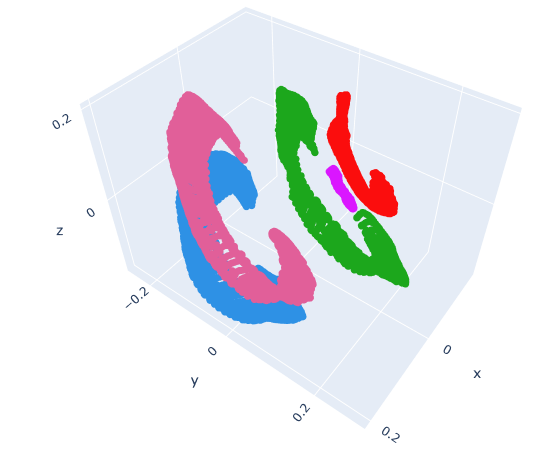
\includegraphics[width=\textwidth]{figures/embeddings/VGG16-3D-block1.png}
    % \caption{Neural manifold preserving spatial ordering.}
\end{subfigure}
\hfill
\begin{subfigure}[b]{0.3\textwidth}
    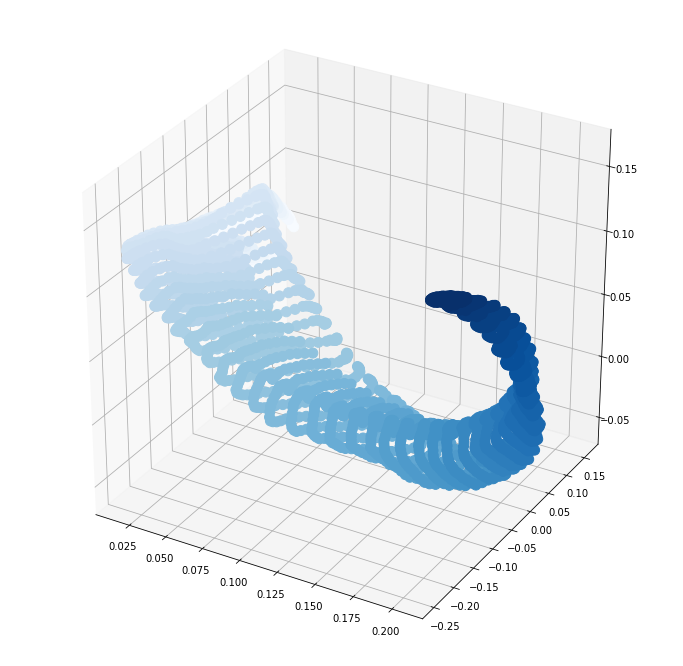
\includegraphics[width=\textwidth]{figures/embeddings/vgg16-spatial1.png}
    % \caption{Neurons colored by vertical order.}
\end{subfigure}
\hfill
\begin{subfigure}[b]{0.3\textwidth}
    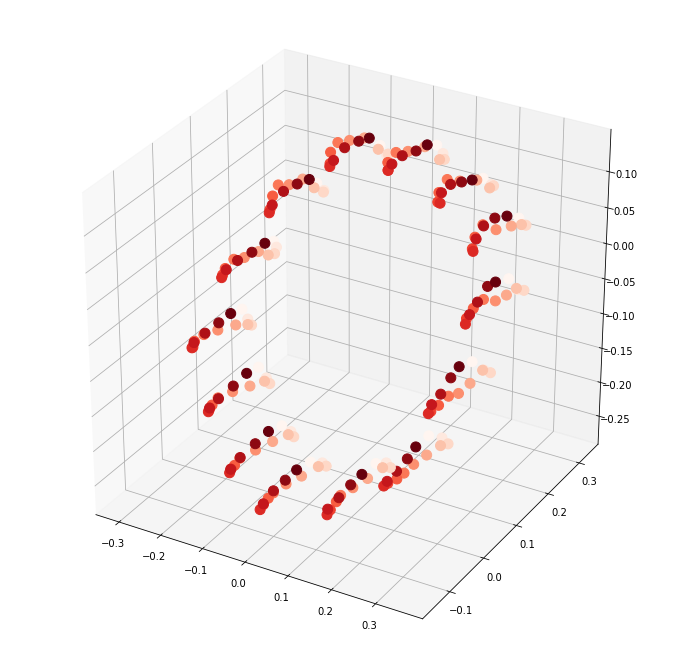
\includegraphics[width=\textwidth]{figures/embeddings/vit-spatial2.png}
    % \caption{Neurons colored by horizontal order.}
\end{subfigure}
\caption{Organization within the CNN neural manifold corresponds to neurons' spatial positions.}
\end{figure}


\section{ViT}

A recent model ViT has been shown to outperform CNN in image recognition tasks while requiring fewer computational resources \cite{vit-vs-cnn}. Transformer \cite{vaswani_attention_2017} is originally designed for sequence-to-sequence tasks primarily used in Natural Language Processing (NLP). In ViT, the given input image is divided into a sequence of 16-by-16 image patches, which allows the image recognition problem to be solved with Transformer. The distinguishing feature of the Transformer model is entirely built on the self-attention mechanisms without using sequence-aligned recurrent architecture.


\subsection{``Individual neuron" in ViTs}
The challenge in building artificial neural tensor for ViT lies in setting up a reasonable analogy to CNN. To do this, we need to scrutinize the structure of ViT. 
\begin{figure}[H]
    \centering
        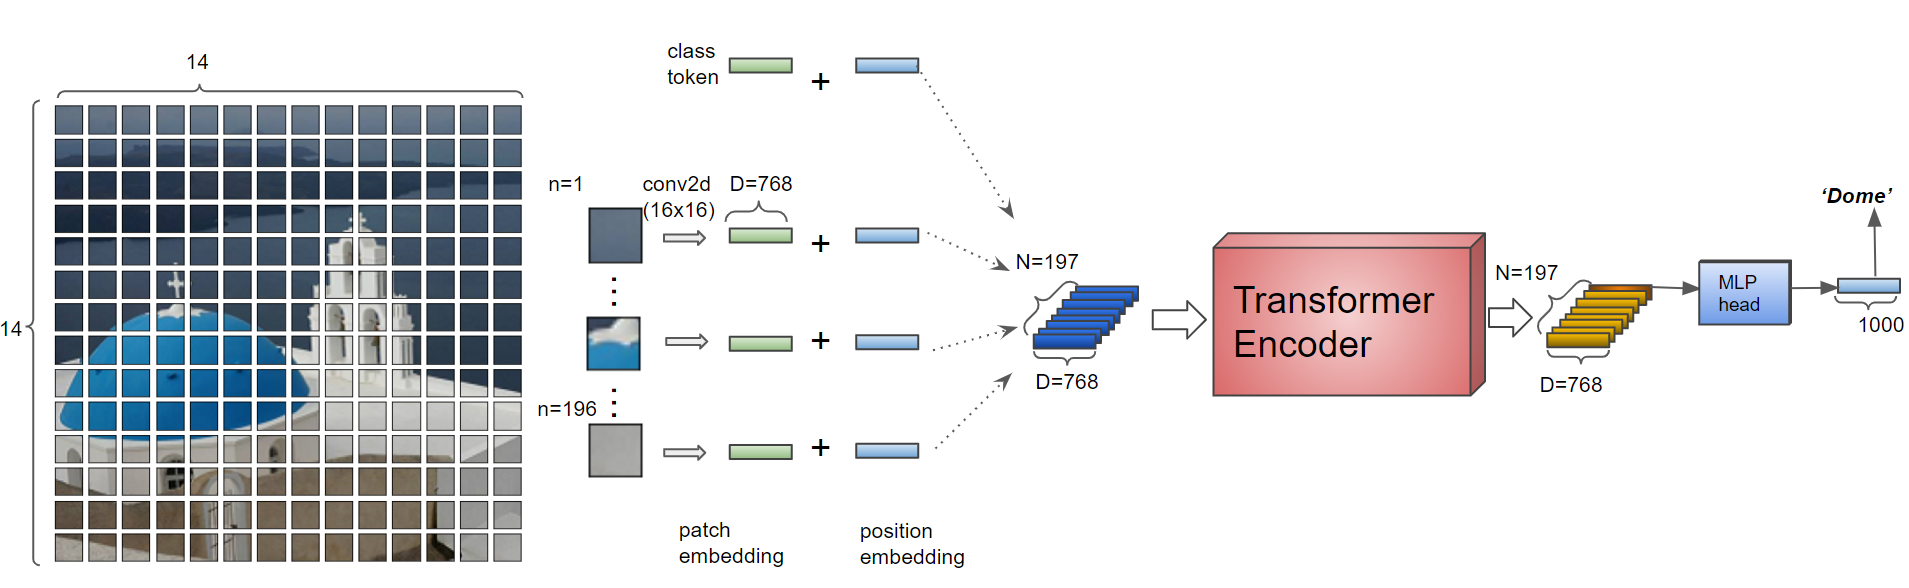
\includegraphics[width=\textwidth]{figures/artificial/vit_input.png}
        \caption{ViT input (image credit: Hiroto Honda).}
\end{figure}
    \begin{figure}[H]
    \centering
        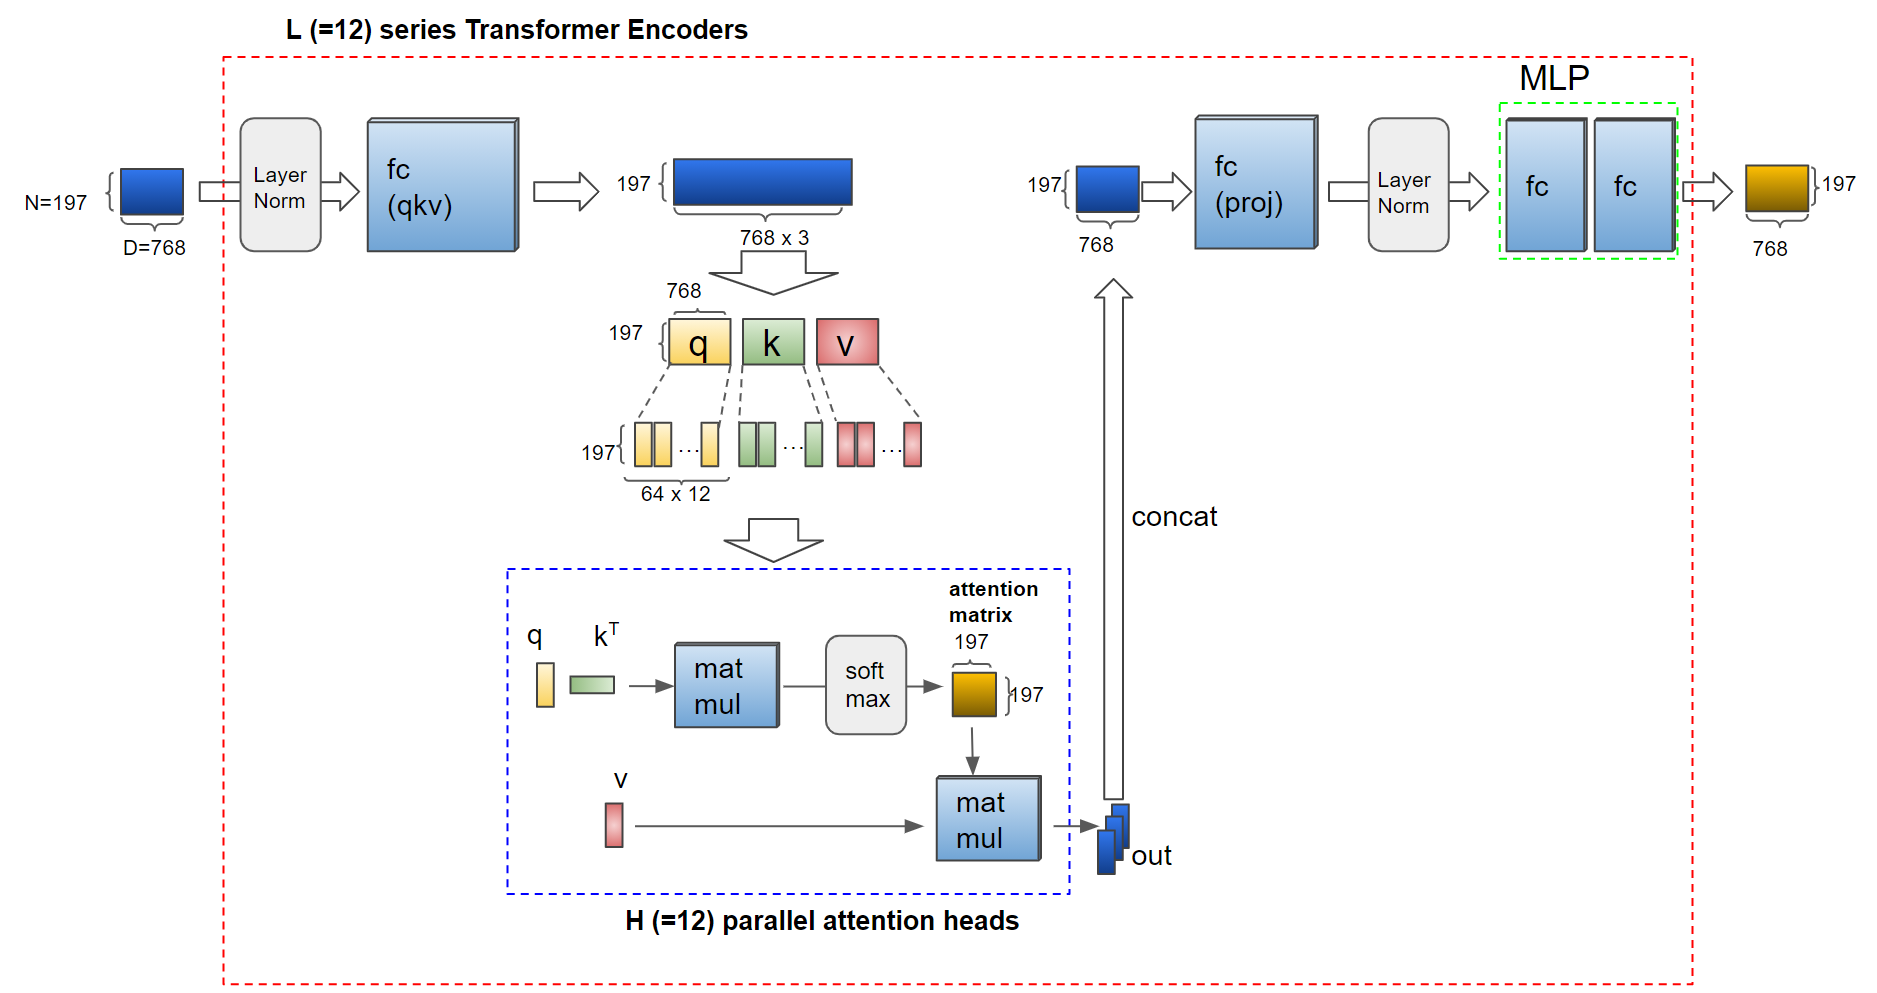
\includegraphics[width=0.8\textwidth]{figures/artificial/vit_encoder.png}
        \caption{ViT encoder (image credit: Hiroto Honda).}
\end{figure}

The following diagram compares the structures of ViT and CNN, which suggests the modification we need to make for ViT based on the previous algorithm for CNN.

\begin{figure}[H]
\centering
\begin{subfigure}[b]{0.45\textwidth}
    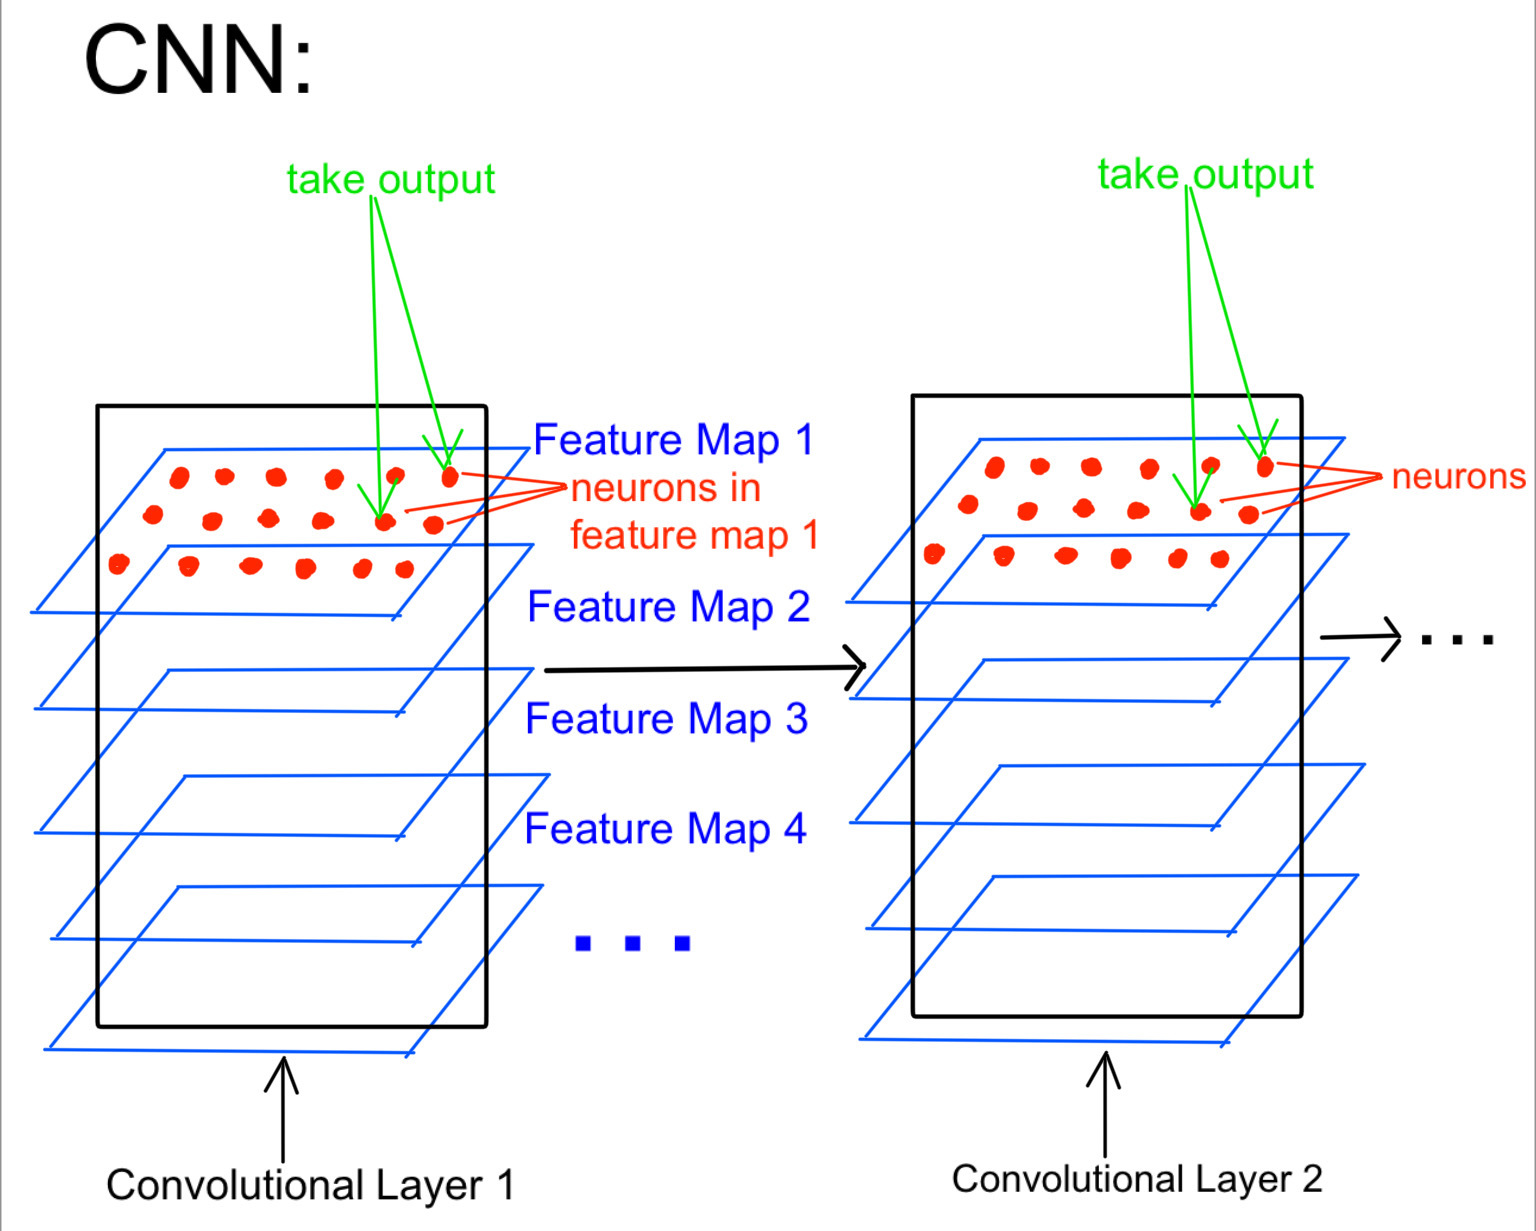
\includegraphics[width=\textwidth]{figures/artificial/cnn-tensor.jpg}
    \caption{Taking neuron output from CNN to build the corresponding neural tensor.}
\end{subfigure}
\hfill
\begin{subfigure}[b]{0.5\textwidth}
    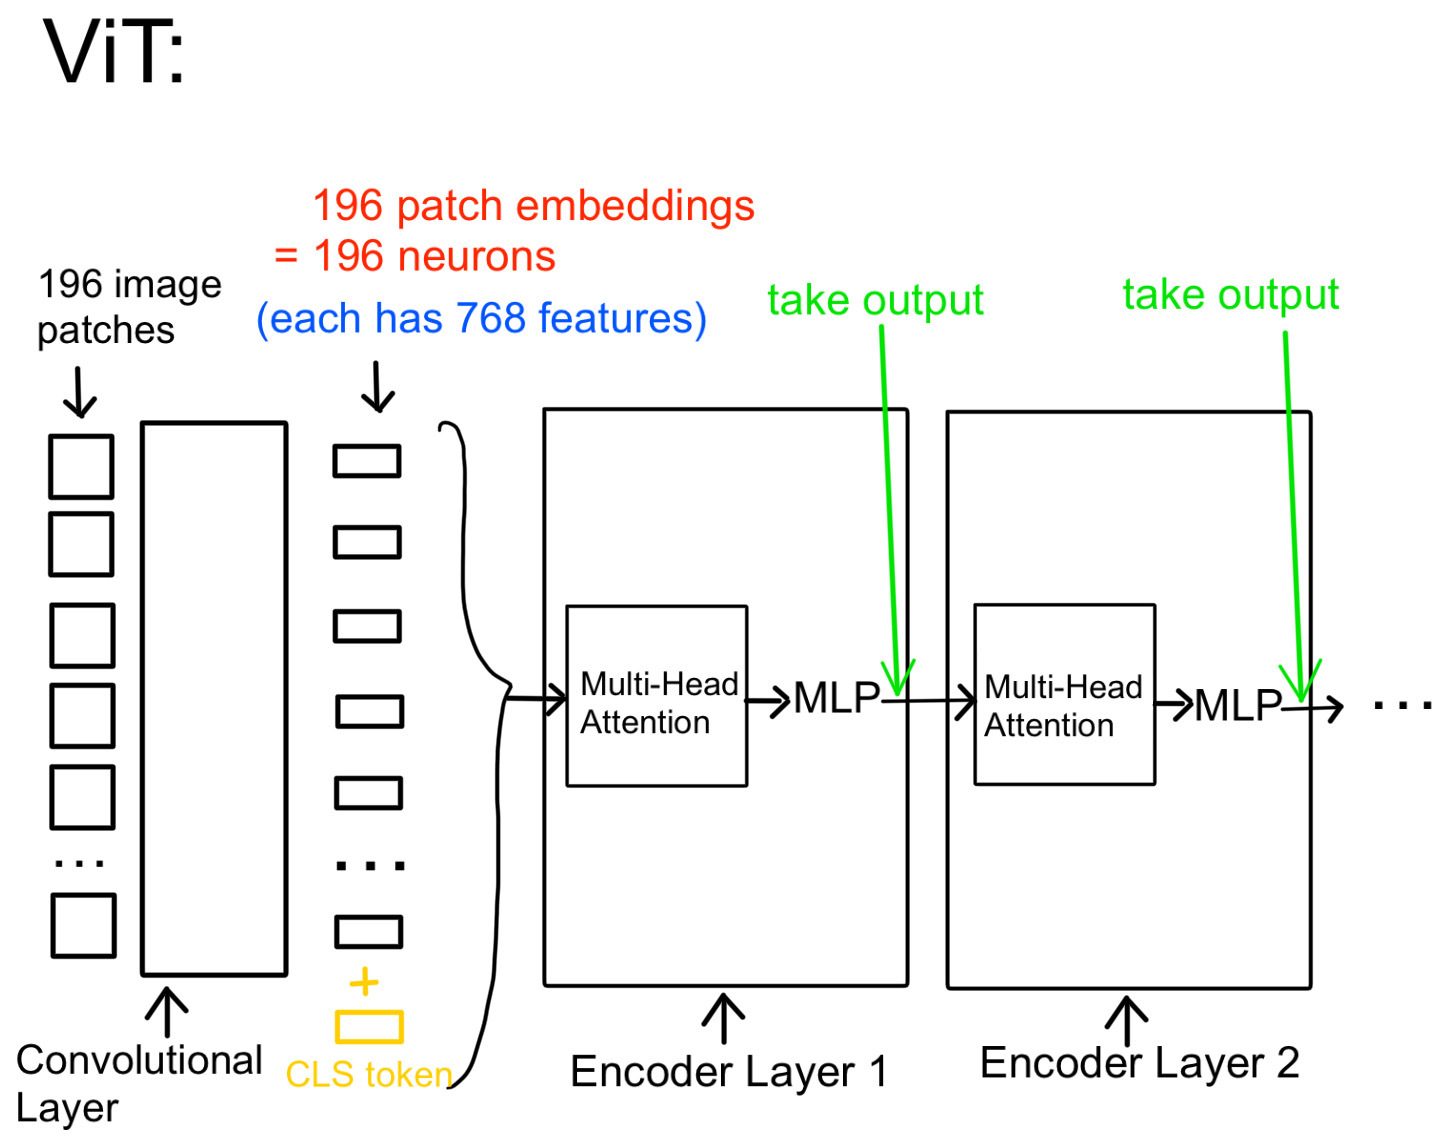
\includegraphics[width=\textwidth]{figures/artificial/vit-tensor.jpg}
    \caption{Taking neuron output from ViT to build the corresponding neural tensor.}
\end{subfigure}
\end{figure} 
Using Algorithm \ref{alg:vit-tensor}, we generate the neural manifold for ViT by taking the output from each encoder layer. The manifold structure for ViT is similar to that of CNN: the manifold is discontinuous and shows discrete clusters organized based on the features obtained from the convolutional layer before the encoder layers. 

\setcounter{algocf}{2}
\begin{algorithm}[H]
\setstretch{1}
\caption{Algorithm for ViT artificial neural tensor.}\label{alg:vit-tensor}
\DontPrintSemicolon
% Set Function Names
  \SetKwFunction{FOutput}{compute\_neuron\_output}
  \SetKwProg{Fn}{Function}{:}{}
  \Fn{\FOutput{$model$, $image\_all\_shifts$}}{
        \For{layer in all encoder layers}{
        pass the image through the model\;
        take the neuron output from the specified layer\;
        apply ReLU activation on the neuron output\;
        compute the average of neuron outputs in each feature\;
        select the feature maps with highest average \;
        normalize the neuron outputs in each feature map\;
        }
  }
\end{algorithm}

\begin{rmk}
On line 5, we need to impose ReLU\footnote{ReLU: Rectified Linear Unit \cite{relu}.} activation to make the neuron output non-negative. The non-negative constraint is desired because the tensor factors from NTF are more interpretable. The pre-trained ViT uses GELU\footnote{GELU: Gaussian Error Linear Unit \cite{gelu}.} as the activation function. This results in negative values and would prevent us from using non-negative tensor decomposition. Fortunately, the negative portion of GELU is negligible given the purpose of our investigation, which justifies this step.
\end{rmk}

An interesting observation is that from shallow layer to deep layer, the sizes of clusters mostly remain the same except for their relative positions, which is slightly different from what is observed for CNN. We provide one possible explanation for this observation. The key mechanism in ViT is self-attention while the key mechanism in CNN is convolution. A crucial difference between the two mechanisms is the receptive field size. Based on findings from \cite{raghu_vision_2021}, \cite{coatnet_2021}, convolution receptive fields are highly local and grow gradually whereas self-attention has global receptive field. As a result, ViT has more uniform representations and greater similarity between lower and deeper layers. 

\begin{figure}[H]
\centering
\begin{subfigure}[b]{0.43\textwidth}
    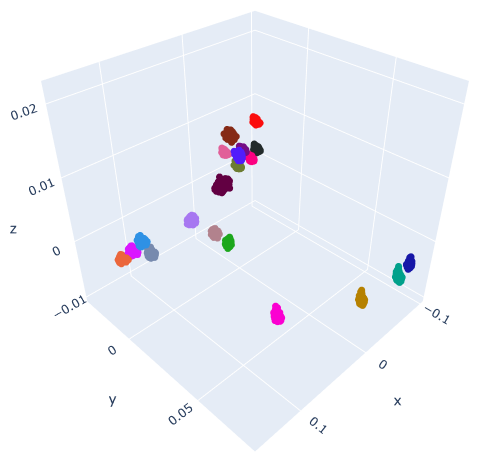
\includegraphics[width=\textwidth]{figures/embeddings/vit-2d-layer1.png}
    \caption{ViT neural manifold (shallow layer).}
\end{subfigure}
\hfill
\begin{subfigure}[b]{0.4\textwidth}
    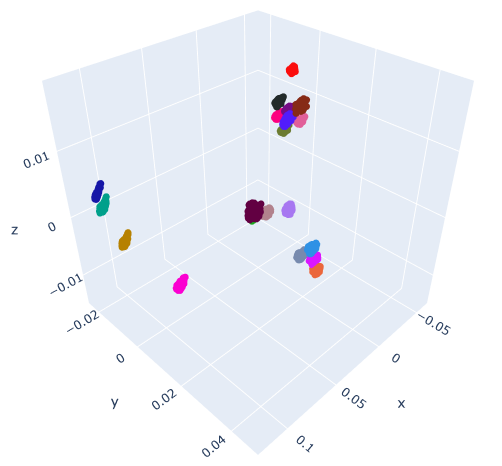
\includegraphics[width=\textwidth]{figures/embeddings/vit-2d-layer12.png}
    \caption{ViT neural manifold (deep layer).}
\end{subfigure}
\end{figure}

We also visualize the neural manifold for ViT that preserves the spatial information, which shows that similar to CNN, neuron responses in ViT also have similar spatial organization within the neural manifold. This similarity is likely because ViT encoder layer takes the features from the convolutional layer as its input.
\begin{figure}[H]
\centering
\begin{subfigure}[b]{0.37\textwidth}
    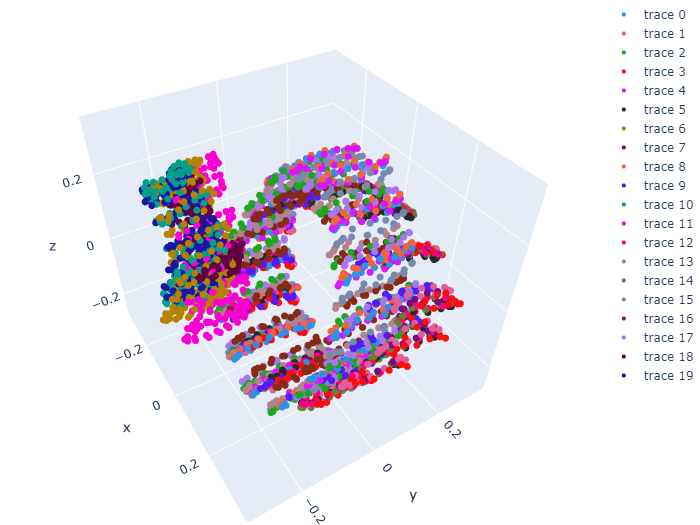
\includegraphics[width=\textwidth]{figures/embeddings/vit-3d-layer1.png}
    % \caption{Neural manifold preserving spatial ordering.}
\end{subfigure}
\hfill
\begin{subfigure}[b]{0.3\textwidth}
    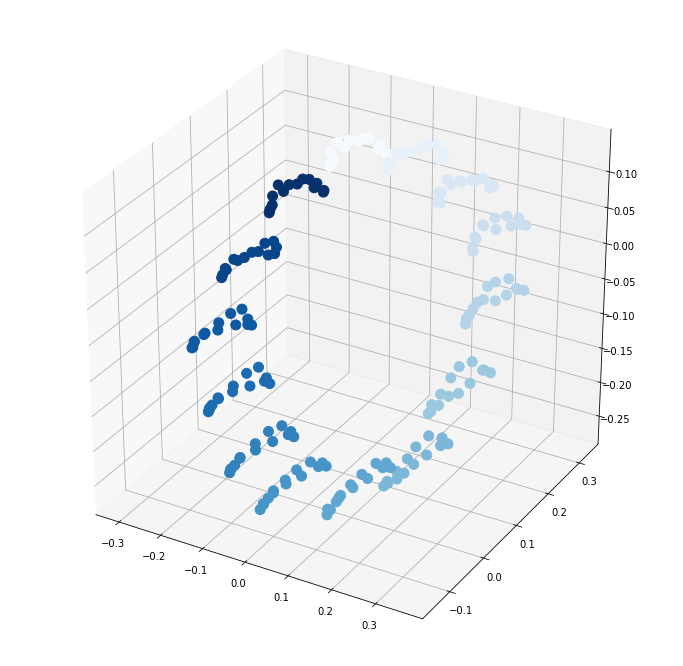
\includegraphics[width=\textwidth]{figures/embeddings/vit-spatial1.png}
    % \caption{Neurons colored by vertical order.}
\end{subfigure}
\hfill
\begin{subfigure}[b]{0.3\textwidth}
    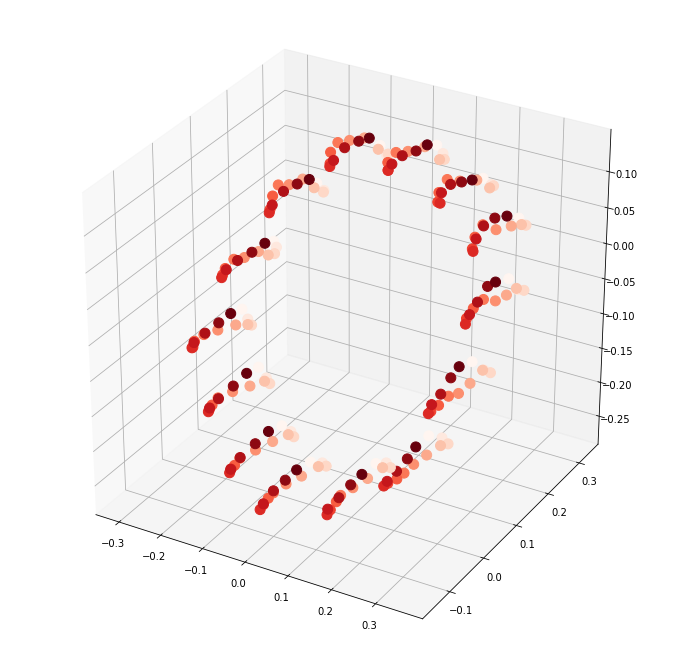
\includegraphics[width=\textwidth]{figures/embeddings/vit-spatial2.png}
    % \caption{Neurons colored by horizontal order.}
\end{subfigure}
\caption{Organization within the ViT neural manifold corresponds to neurons' spatial positions.}
\end{figure}

\subsection{Quantifying the continuity of the manifold}

Following the method proposed in \cite{dyballa_manifold_2021}, we further compute the MFR as we have done for biological neural networks. Since it is clear from the visualization that the neural manifolds CNN and ViT are similarly discontinuous, it suffices to compute the MFR for one of them. We compare the respective neural manifolds and their respective MFR for CNN, retina, and V1:

\begin{figure}[H]
\centering
\begin{subfigure}[b]{0.3\textwidth}
        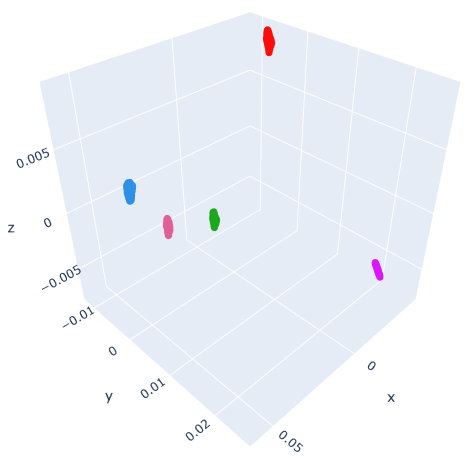
\includegraphics[width=\textwidth]{figures/embeddings/VGG16-2D-block1.png}
        \caption{$\phi_G = 0.27$ for CNN.}
\end{subfigure}
\hfill
\begin{subfigure}[b]{0.3\textwidth}
        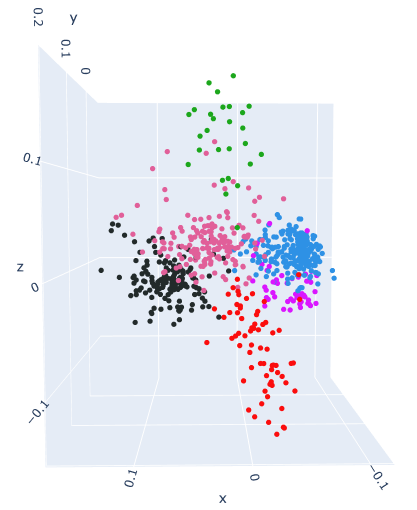
\includegraphics[width=\textwidth]{figures/biological/retina-manifold.png}
        \caption{$\phi_G = 0.56$ for retina.}
\end{subfigure}
\hfill
\begin{subfigure}[b]{0.3\textwidth}
        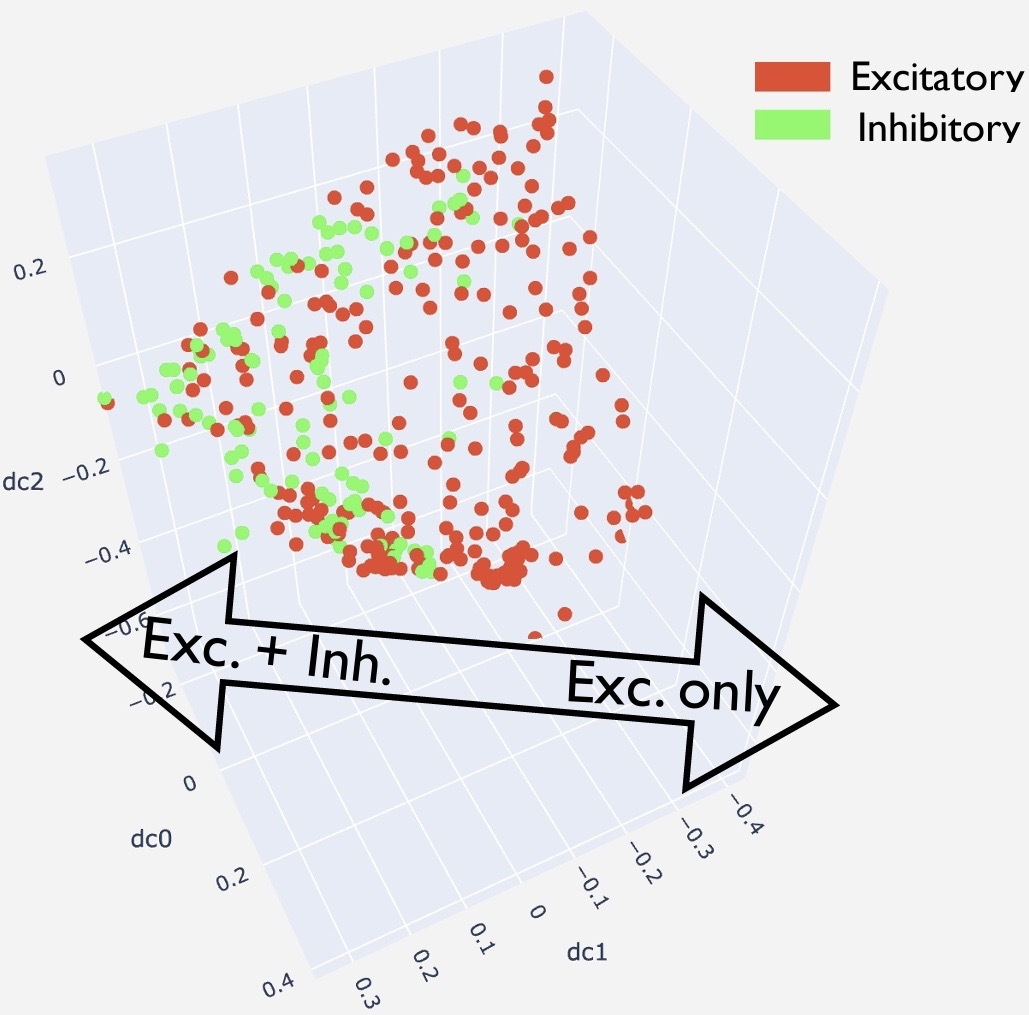
\includegraphics[width=\textwidth]{figures/biological/v1-manifold.jpg}
        \caption{$\phi_G = 0.91$ for V1.}
\end{subfigure}
\end{figure} 
% \begin{figure}[H]
% \centering
%     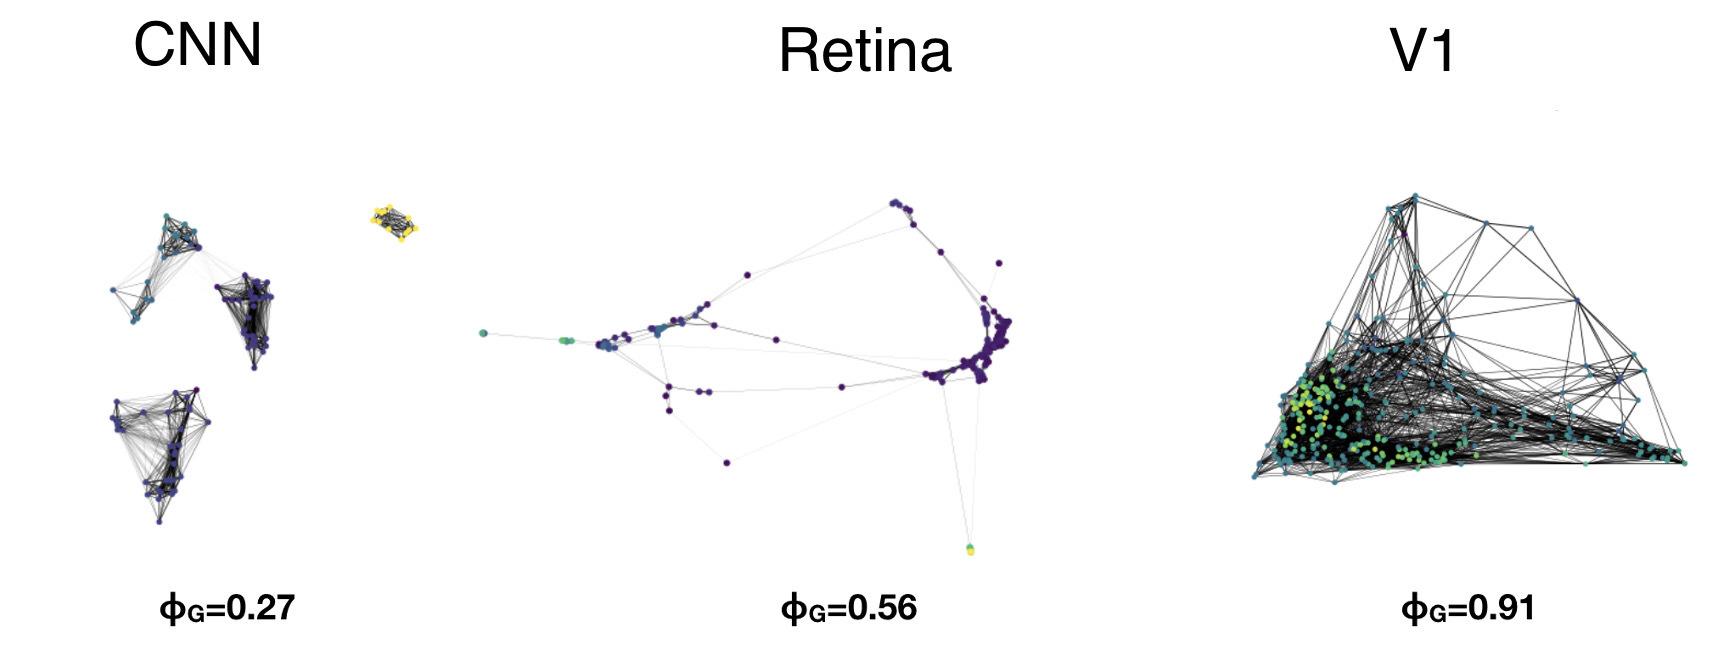
\includegraphics[width=0.75\textwidth]{figures/embeddings/mean-flow-ratio-results.jpg}
% \caption{Comparing the mean flow ratio of CNN with that of the biological neural networks in retina and V1.}
% \end{figure}
The quantitative comparison aligns with our qualitative comparison: from the visualization, we have observed that V1 has a much more continuous manifold than CNN and the retina; similarly, the MFR of V1 is notably higher than CNN and the retina. MFR additionally reveals (which is not entirely obvious from the visualizations) that there seems to be a considerable gap between between CNN and retina as well.

\section{Adding recurrence}
Since neither the convolution in CNN nor the attention mechanism in ViT yields continuous neural manifold like V1, this leads us to investigate other computational mechanisms that could result in a more continuous neural manifold. Based on our literature review in \ref{neuro-recurrent}, we hypothesize that recurrent models might be promising. For this reason, we apply the same method to investigate computer vision models with recurrent structures. One challenge is that recurrent neural networks (RNNs) themselves are not commonly used for image recognition tasks. Fortunately, there are computer vision models that combine convolution and recurrent units. For this reason, we choose two representative models: first, convolutional RNN (CRNN) \cite{convrnn_shi_end--end_2015} that adds recurrent layers after the convolutional layers and second, $\gamma$-net \cite{serre-recurrence} that adds recurrent connections directly on the convolutional layers. Algorithm \ref{alg:cnn-tensor} for CNN applies in this case as well. We include here our preliminary findings for neural manifold obtained from CRNN \cite{convrnn_shi_end--end_2015}.  
\begin{figure}[H]
\centering
    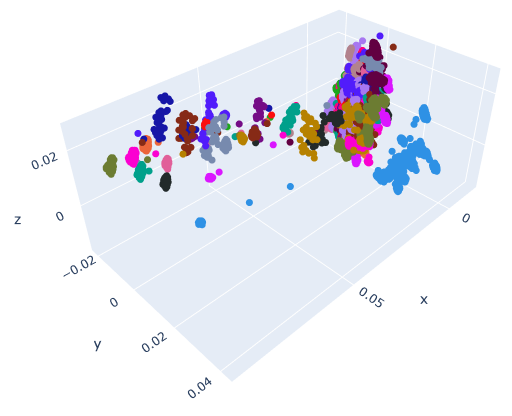
\includegraphics[width=0.5\textwidth]{figures/embeddings/crnn-2d-layer1.png}
\caption{Neural manifold for CRNN (shallow layer).}
\end{figure}
As observed from the figure above, the clusters become less separated and  ignificantly overlap with each other, which is in contrast to the neural manifolds for CNN and ViT . This suggests that by adding the recurrently layers and jointly training the unified network we can obtain a more continuous manifold. A possible reason for this observation is that due to the structure of this model, the convolutional layers are affected by the recurrent units in the RNN layers in that the RNN layers can back-propagate error differentials to its inputs from the convolutional layers. 

Another intriguing result is that when visualizing the neural factors (obtained by applying NTF on respective neural tensors), the neural factors for CRNN seem to have very distinct properties from those for CNN and ViT. The neural factors visualize the independent neural firing patterns that can approximately summarize all the neural firing patterns in the original neural tensor. In the following figure, we see that the for CNN and ViT there is mostly just one bright region in each factor, suggesting that the neurons mostly respond to a single targeted feature/region in the input image. This likely implies the neurons have strong stimuli preferences and they participate in isolated neural circuits (thus yielding a continuous manifold). However, neural factors for CRNN indicate some sequential patterns with many bright regions in each factor, suggesting that the neurons might respond to multiple stimuli. This implies that the underlying neural circuit is more interconnected, which is why we have observed a more continuous manifold.
\begin{figure}[H]
\centering
\begin{subfigure}[b]{0.4\textwidth}
        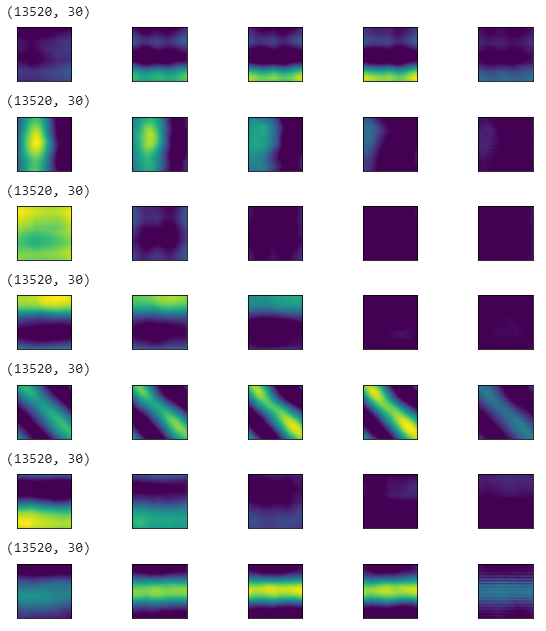
\includegraphics[width=0.85\textwidth]{figures/artificial/cnn-factor.PNG}
        \caption{Neural factors for CNN.}
\end{subfigure}
\hfill
\begin{subfigure}[b]{0.57\textwidth}
        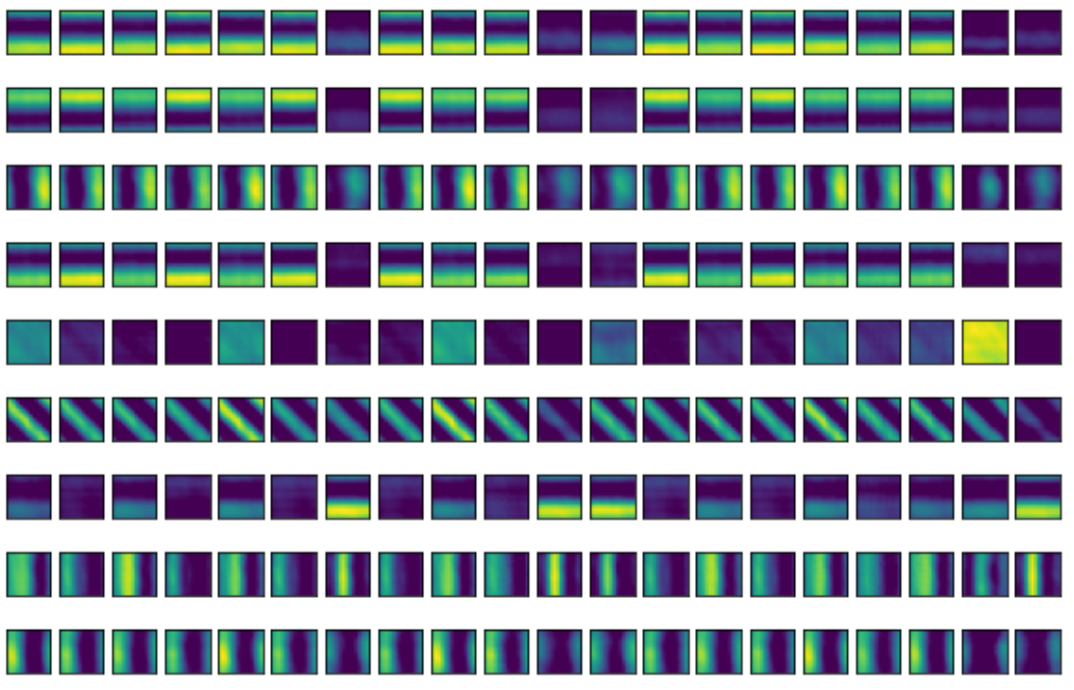
\includegraphics[width=\textwidth]{figures/artificial/vit-factor.PNG}
        \caption{Neural factors for ViT.}
\end{subfigure}
\end{figure} 
\begin{figure}[H]
\centering
    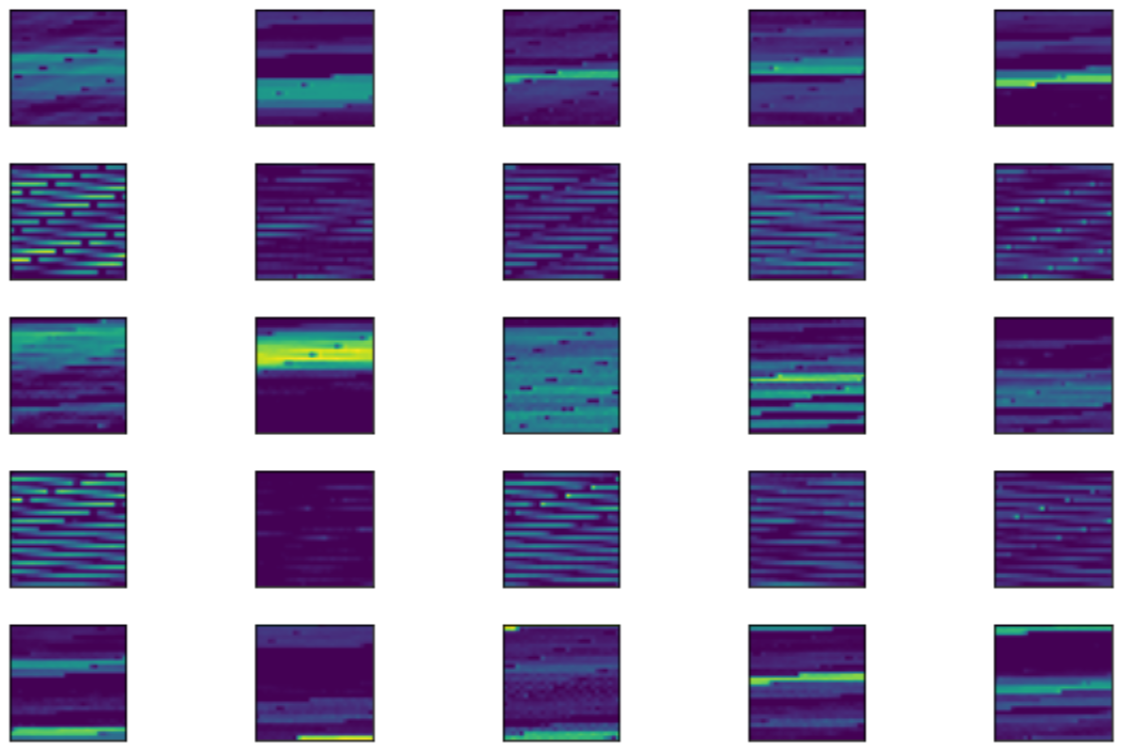
\includegraphics[width=0.45\textwidth]{figures/artificial/crnn-factor.png}
    \caption{Neural factors for CRNN are distinct from CNN and ViT.}
\end{figure}

\chapter{Conclusion}
\label{chapter-conclusion} 

\section{Summary and discussion of results}
Our results were the first to show that CNN and ViT form discontinuous neural manifold whereas adding recurrent units to the network forms a more continuous manifold. From this we can infer that  CNN and ViT form isolated neural circuits and recurrent connections increase the connectivity of the underlying neural circuits. We reformulate our results in terms of conjectures that address the open questions raised in section \ref{intro-motivation}:
\begin{itemize}[noitemsep, topsep=0pt]
    \item \textit{How do computer vision models (VGG16 \cite{vgg16_simonyan_very_2015}, Vision Transformer \cite{vit_dosovitskiy_image_2021}, and Convolutional Recurrent Neural Network \cite{convrnn_shi_end--end_2015}) compare to biological vision, specifically in the regions retina and V1?} 
    
    \textbf{Conjecture 1.} The underlying neural circuits in feed-forward networks, including CNN and ViT, are closer to that in retina than that in V1. In other words, they are decent models for retina but are severely limited as models for V1.
    
    \item \textit{What specific feature(s) in computer vision models lead to the differences in the neural circuits?}
    
    \textbf{Conjecture 2.} Incorporating recurrent mechanisms in computer vision models seems to be crucial in increasing the connectivity of the underlying neural circuits.
\end{itemize}

The implication of \textbf{Conjecture 1} is that, contrary to popular belief, current computer vision models turn out to be poor approximations of visual cortical circuits (although they are indeed inspired by early studies of the visual cortex and perform well on image recognition tasks). These feed-forward networks are good enough as models for the retina, but fail to capture the characteristics of the functional neural circuits in the visual cortex. \textbf{Conjecture 2} suggests that recurrence seems to be the missing key to a more accurate model of the visual cortex. In the next section, we will propose future research in three directions:

\section{Future directions}
\subsection{Understanding the role of recurrence in vision}
Recurrence is a characteristic feature in not only biological vision but also most of our important brain functions. However, recurrence is largely missing from most of the popular computer vision models today. Our results have suggested that recurrence is key to increasing the connectivity of the underlying functional neural circuits in the neural networks (both artificial and biological). Since richer functional connectivity is a desirable feature for neural networks when solving visual tasks that involve more complex reasoning, it could potentially have significant implication in advocating the merit of incorporating recurrent mechanisms into computer vision models. Thus, we propose a more extensive analysis of the role of recurrence in both biological vision and computer vision. 

\subsection{Experimenting with recurrent models}
The experiments in Chapter \ref{chapter-artificial} have solved some open questions that we set out to tackle, but they also leave us with many more intriguing observations that we have not understood fully. Building on the results we have obtained during the capstone, we will continue and focus on studying how various recurrent structures affect the the neural manifold. We are currently in the process of obtaining an additional pre-trained network model \cite{serre-recurrence}, which includes recurrent connections directly to the convolutional layers. Our current investigation on the neural manifold of artificial neural networks with recurrent structures is still limited: we have only studied CRNN which add recurrently layers after the convolutional layers. This might not be sufficient and we believe that the model in \cite{serre-recurrence} that adds recurrence directly to the convolutional layers would be a promising place to continue. It would be of interest to find out whether (and if so, why) adding recurrence in different ways may result in manifolds with different structure. We can apply the mean flow algorithm to precisely quantify the extent to which each kind of recurrent structure change the continuity of the neural manifold.

\subsection{Applying nonlinear dimensionality reduction}
Although the linear dimensionality reduction method (tensor CP decomposition) has been working well so far, this could be a potential limitation of our current study, especially since that both network science and neural dynamics are typical contexts where nonlinear systems arise. It might be interesting to apply the nonlinear dimensionality reduction method (diffusion map) to compare the results.  

\appendix 


\renewcommand*{\bibfont}{\footnotesize}
\setlength\bibitemsep{0pt}
\begin{singlespacing}% \printbibliography[heading=bibintoc]
% \bibliography{biblio}[title=Bibliography (Main)]
\printbibliography[title=Bibliography (Main), heading=bibintoc, keyword=main]
\printbibliography[title=Bibliography (Supplementary), heading=bibintoc, notkeyword=main]
\end{singlespacing}


% ----------------------------------------------------------------------------------------
% 	QUOTATION PAGE
% ----------------------------------------------------------------------------------------
\clearpage
\thispagestyle{empty}
\vspace*{0.2\textheight}

\noindent\enquote{\itshape In a shorter time, more will be known about the most remote objects, namely the stars, than about the most nearby topic, namely perception. }\bigbreak

\hfill Aristotle
\clearpage
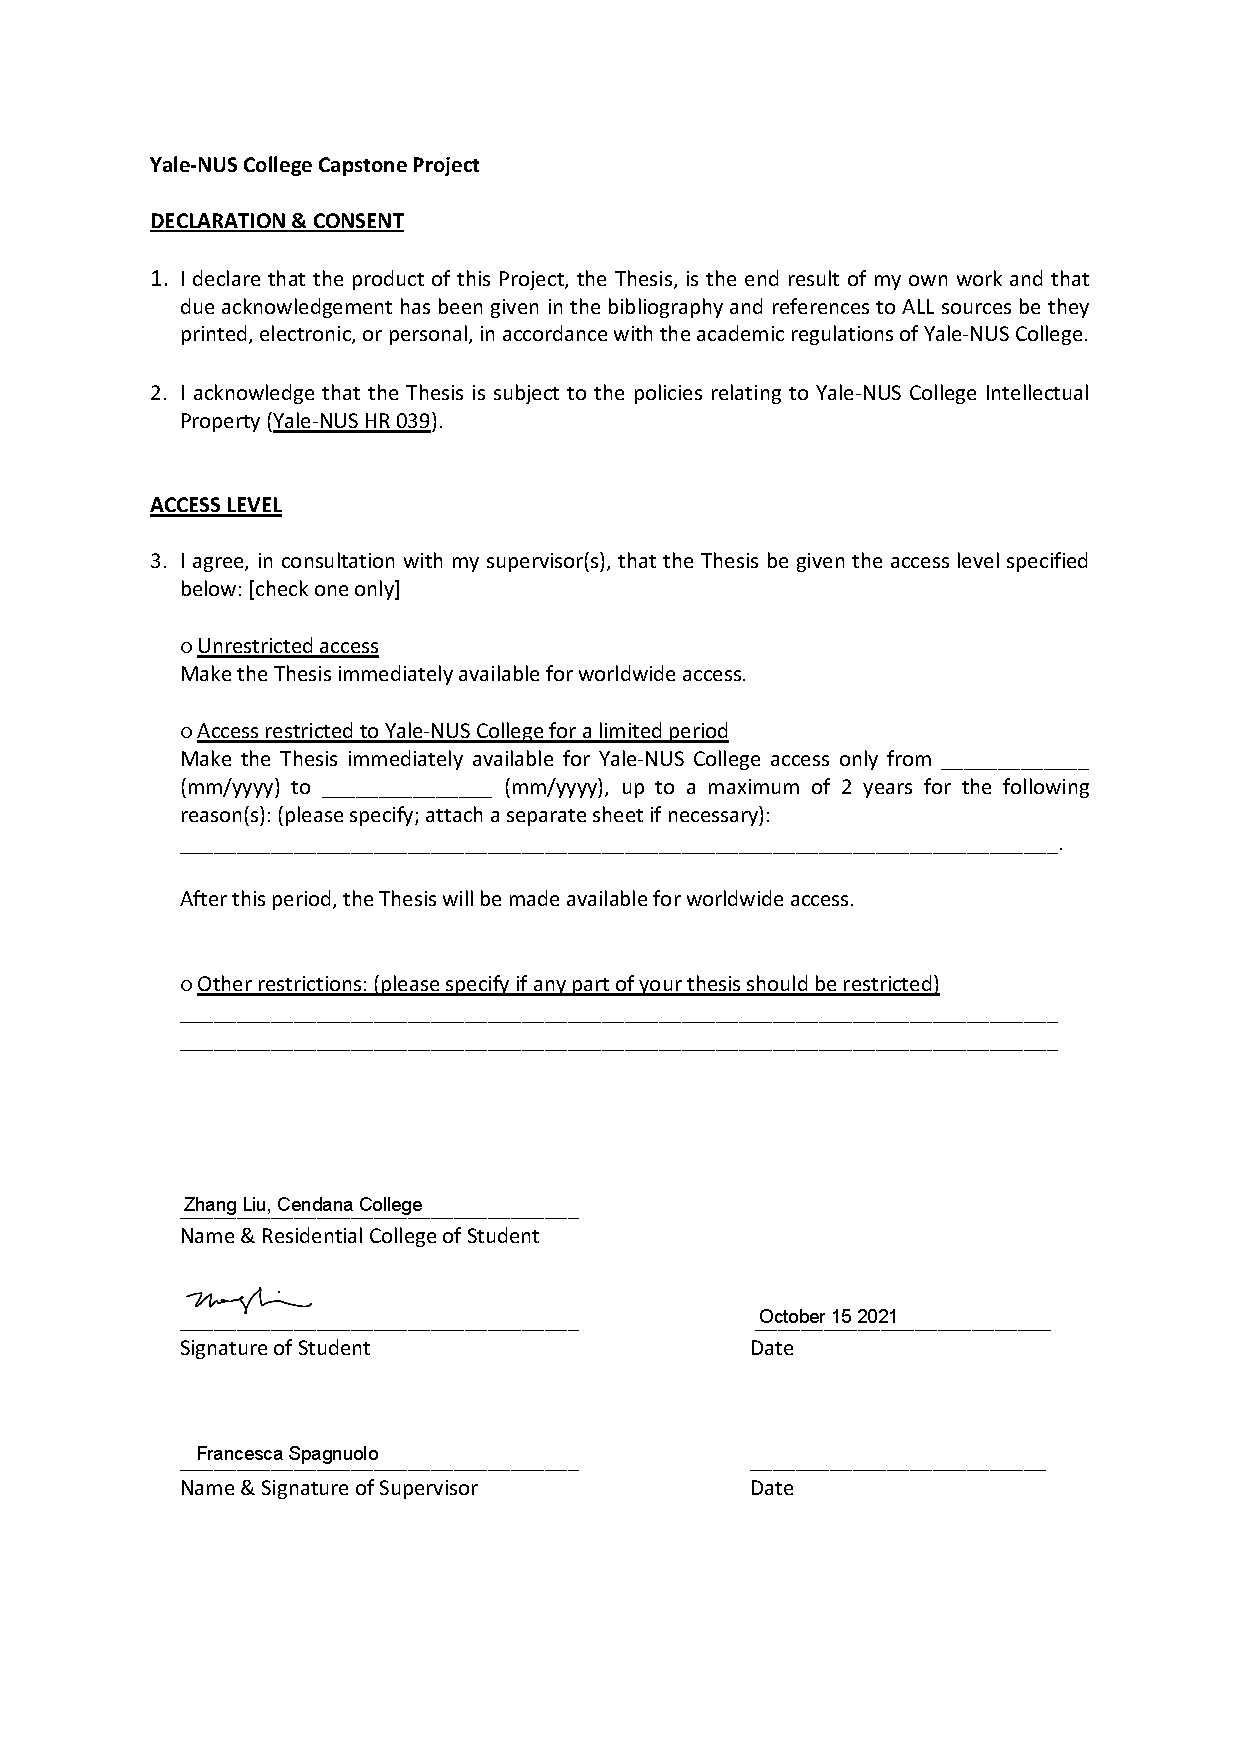
\includepdf[pages=-,pagecommand={},width=\textwidth]{declaration.pdf}
\begin{acknowledgements}
\addchaptertocentry{\acknowledgementname} 
    I would like to thank my supervisor Francesca Spagnuolo  and co-supervisor and mentor Steven W.~Zucker and Luciano Dyballa for their generous guidance and advice. They have made possible the many serendipitous moments in this project. There have been ups and downs in this project, but their support has helped me keep a keen spirit for learning and discovery. To the faculty at Yale-NUS for nurturing me into a good human being, and for bearing with my countless weaknesses and mistakes, particularly the MCS faculty who have had paramount influence in my development as a researcher: Prof.~Francesca Spagnuolo, Prof.~Olivier Danvy, Prof.~David Smith, Prof.~Robby Tan, and  Prof.~Timothy Wertz. Remarkably, they somehow believed in me even in times when I myself did not and provided me with the right guidance. To my family, thank you for loving me for who I am. To my suitemates, friends, and alumni, thank you for patiently bearing with my endless sharing of my work and ideas. Specifically, I acknowledge Xiyao Fu, Aparna Gupte, Mark Yuen for providing feedback; almuni Abhinav Natarajan, Dion Ho, Sultan Aitzhan, Yiming Ng, Wei Han, Xin Run for supporting me throughout my college years; friends whom I have had conversations with about this capstone: Amanda Leong, Zhala Sarmast, Amberly Yeo, Glenda Chin, Dasha Haryfullina, Aiman Imtiaz, Lize Cai, Yanhua Wang, Linda Li, Jia Tang, Eric Lan, \dots To the trees on campus, thank you for being there and reminding me of the life force within me. To whoever has read thus far, it's my pleasure to take you on this short tour with me. I have flaws, and my thesis has flaws - I sincerely invite more conversations about them. 
    %  
\end{acknowledgements}

\chapter{Complete List of Experiments}
\label{appendix-all-experiments}
I have also conducted many exploratory experiments. A complete list of the experiments are included below.
For the biological neural tensor, I conducted the following experiments:
\begin{enumerate}
    \item applying tensor CP decomposition to generate the neural manifold
    \item applying diffusion map to generate the neural manifold
    \item applying persistent homology and Wasserstein distance to compare the topological features of the neural manifold
    \item over training AlexNet
\end{enumerate}

For the artificial neural tensor, I conducted the following experiments:
\begin{enumerate}
    \item building the artificial neural tensor without considering shifts in images
    \item building the artificial neural tensor with shifts in images
    \item applying tensor CP decomposition on the artificial neural tensor (with shifts in images)
    \item studying how the neural manifold changes during the training of an ANN (instead of using the pre-trained ANN)
    \item applying persistent homology (though with limited explainability)
\end{enumerate}


\label{appendix-lists}
\setcounter{tocdepth}{2}
\listoffigures
 \listofalgorithms
 \listoftables
\chapter{Diffusion Map} 
\label{appendix-diffmap} 

Besides tensor CP decomposition, we also explore the non-linear dimensionality reduction method of diffusion map. (Note that most of the results presented in this report can be obtained from tensor CP decomposition. However, when the former failed to provide meaningful results, we turn to the diffusion map.) The main references for this section are \cite{coifman_geometric_2005},   \cite{coifman_diffusion_2006} and \cite{stanley_geometric_2020}. We will now outline the steps in the diffusion map algorithm.
\begin{enumerate}
\item Discretize the underlying manifold as a weighted graph.
\begin{defn}[Discretization of a manifold]

Given $X = \{x_1, x_2,\dots, x_n\}$, a set of data sampled from a Riemannian manifold $\mathcal{M}$, we can construct the discretization of $\mathcal{M}$ as as a weighted, undirected graph, $\mathcal{G}_X = (X, g_\epsilon)$ where $X$ is the set of vertices given by the data and $g_\epsilon$ is a Gaussian kernel function $g_\epsilon: (x_i, x_j) \to [0,\infty]$ defined by the following rule
\begin{align}
    g_\epsilon(x_i,x_j) = \frac{1}{2}\left(\exp{\frac{-\|x_i - x_j\|_2^2}{2\epsilon(x_i)}} + \exp{\frac{-\|x_i - x_j\|_2^2}{2\epsilon(x_j)}}\right), \quad \forall x_i,x_j \in X, 
\end{align}

 where $\epsilon: X \to \RR$ is the the bandwidth function by which the Gaussian kernel is parameterized. 
\end{defn}

Gaussian kernel is only one of the possible kernel functions, but it gives a physically intuitive construction for learning the manifold underlying the data sample because it effectively considers a ball of radius $\epsilon$ around each data point.

The choice of $\epsilon$ determines the radius of neighborhood of $x_i \in X$. $\epsilon$ is application-specific and is usually a global bandwidth, that is, $\epsilon(x_i) = \epsilon(x_j)$ for all $x_i, x_j \in X.$ 

\item Compute the similarity matrix associated with the weighted graph.

Given the weighted graph $\mathcal{G}_X$, we can compute the corresponding similarity matrix. Each entry in the similarity matrix, $W_{i j}$, is the pairwise similarity value between data/vertices $x_i$ and $x_j$ and is taken as the weight of the edge between nodes $x_i$ and $x_i$. 
    \begin{align}
        W_{i j } = \exp\{-\frac{\|x_i - x_j\|^2}{2\sigma^2}\}.
    \end{align}
    
\item Construct a lazy random walk on $\mathcal{G}_X$. 

First, we define random walk on the weighted, undirected graph $\mathcal{G}_X$: 

\begin{defn}[Random walk on graphs]
A \underline{random walk} on $\mathcal{G}_X = (X,g_\epsilon)$ is a process that begins at some vertex $x_i$, and at each time step moves to another vertex $x_j$. Since the graph is weighted, it moves to a neighbor $x_j$ with probability $p(j \mid i)$, proportional to the weight of the corresponding edge, and is defined as follows:
\begin{align}
        p(j\mid i) = \frac{W_{i j}}{\sum_{k} W_{i k}}.
\end{align}
The random walk is \underline{lazy} if we allow $p(i\mid i) > 0$, i.e., the probability of staying at some point $i$ as the time step moves forward is non-zero.
\end{defn}
    
    The probabilities $p(j \mid i)$ can be represented by a Markov matrix $M$, which is essentially the similarity matrix normalized to have row sums equal to $1$:
     \begin{align}
        M = D^{-1} W, \text{where } D_{i i} =\sum_{k}W_{i k}.
    \end{align}
    The probability of reaching node $x_j$ from $x_i$ after $t$ steps is then
    \begin{align}
        p(t,j\mid i) = e_i^T M^t e_j.
    \end{align}

    \item Eigendecomposition of the Markov matrix:
    
    The eigendecomposition of $M$ is derived from the eigendecomposition of $M_s = D^{1/2} M D^{-1/2} = \Omega \Lambda \Omega^T$:
    \begin{align}
        M = D^{-1/2}  \Omega \Lambda \Omega^T D^{-1/2} \coloneqq \Psi \Lambda \Phi^T.
    \end{align}
    
    Note that since $\Psi$ and $\Phi$ are mutually orthogonal, $\Psi$ contains the right eigenvectors, as shown below:
     \begin{align}
        M \Psi =  \Psi \Lambda \Phi^T \Psi = \Psi \Lambda =  \Lambda \Psi.
    \end{align}
    
    The eigendecomposition of $M$ after $t$ steps is then
    \begin{align}
        M = \Psi \Lambda^t \Phi^T.
    \end{align}
    \begin{itemize}
        \item Diffusion coordinate functions are the right eigenvectors of Markov matrix scaled by their corresponding eigenvalues: 
        \begin{align}
            \Upsilon \coloneqq \Psi \Lambda.
        \end{align}
        \item Diffusion distance after $t$ steps is the following:
       \begin{align}
            \| e_i^T  \Upsilon - e_j^T \Upsilon  \|^2 = \sum_{k} (p(t,k\mid i) - p(t,k\mid j))^2 (D_{k k}^{-1}).
       \end{align}
       
       \item Infer geometric properties from the growth of eigenvalues of $M$.
       
       For intuition behind the relation between the growth of eigenvalues and the geometric properties of the underlying manifold that we begin with, we consider the following two extreme situations:
       \begin{enumerate}
           \item If the discretization of the underlying manifold is a disconnected graph (none of the nodes are connected), then:
           \[P = I, \lambda_i = \lambda_j \quad \forall i, j, \]
           which implies a flat spectrum with zero decay rate.
           \item If the discretization of the underlying manifold is a fully connected graph (each of the node is connected to all the rest of the nodes), assuming weights of all edges are $1$, then:
            \[\lambda_1 = 1, \lambda_i = 0 \quad \forall i \neq 1.\]
       \end{enumerate}
    \end{itemize}
\end{enumerate}

\par \textbf{Key ideas of diffusion maps: }
\begin{itemize}
    \item The similarity kernel gives us the \textit{local} geometry. As the time steps move forward, we integrate the local geometry and thus reveal the geometric structures at different scales. 
    \item A cluster from a random walk is a region where the probability of escaping this region is low.
\end{itemize}

\section{Demonstration of the method}
As a demonstration of the diffusion maps method, we apply it on synthetic spiral data and MNIST handwritten digits images data:

\begin{figure}[H]
        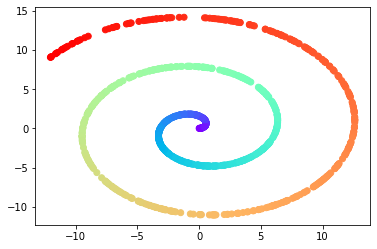
\includegraphics[width=0.6\textwidth]{presentation/spiral.png}
        \caption{Visualising the original spiral data.}
    \end{figure} 
  \begin{figure}[H]         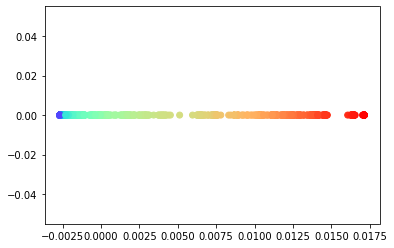
\includegraphics[width=0.6\textwidth]{presentation/spiral-unroll.png}
        \caption{First non-trivial coordinate function.}
        \end{figure} 
\begin{figure}[H]
        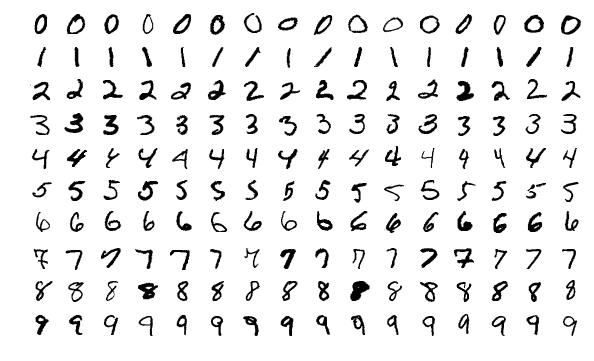
\includegraphics[width=0.4\textwidth]{presentation/mnist-vis.png}
        \caption{Sample data from the MNIST.}
    \end{figure} 
  \begin{figure}[H]
            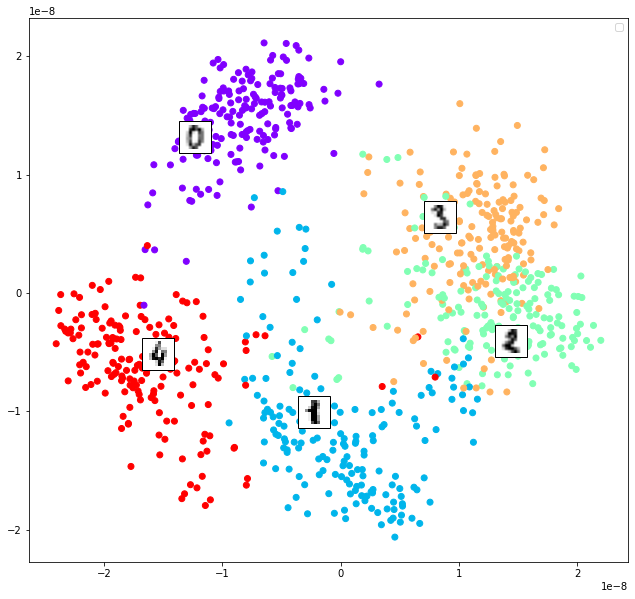
\includegraphics[width=0.6\textwidth]{presentation/mnist.png}
        \caption{First two non-trivial coordinate functions (plotting only five of the digits classes).}    
        \end{figure} 
        
\section{Remarks on non-linear dimensionality reduction}
Setting the right parameters for non-linear dimensionality reduction is very challenging, especially for lab data where sampling errors are prevalent. For this reason, we will be investigating this method in greater details in the second half of the project instead.  

% [to-do: axis set to equal for the plot; and mention only plotting 5 classes]
\chapter{Principal Component Analysis} 
\label{appendix-pca} 

Principal component analysis (PCA) is the simplest matrix decomposition model. The PCA model can be formulated as an optimization problem. Given a $N$-by-$M$ matrix $\mathbf{X}$ with $N$ variables and $M$ features, we can approximate $\mathbf{X}$ with the product of two orthogonal rank-one matrices:
\begin{align}
    \mathbf{X} \approx \mathbf{U}\mathbf{V}^T = \sum_{r=1}^R u_r \circ v_r,
\end{align}
where $\circ$ denotes the outer product operator. The equivalent element-wise formulation of the PCA model is
\begin{align}
\label{pca}
    x_{i j} \approx \sum^R_{r = 1} u_i^r v_j^r.
\end{align}
With PCA, the dimensionality of the original matrix can be reduced from from $N$-by-$M$ to $N$-by-$R$. This can be illustrated with the diagram below
\begin{figure}[H]
    \centering
        \includegraphics[width=0.7\textwidth]{figures/linear/pca.jpg}
        \caption{Illustration for PCA. (Adapted from \cite{williams_unsupervised_2018})}
    \end{figure} 
PCA seeks to solve a sequence of optimization problems:
\begin{itemize}
    \item maximize variance:
\begin{maxi}|l|
  {\mathbf{V}}{\|\mathbf{X}\mathbf{V}\mathbf{V}^T\|_F^2}{}{}
  \addConstraint{\mathbf{V}\text{ orthonormal}},
 \end{maxi}
 \item minimize residuals:
 \begin{mini}|l|
  {\mathbf{U},\mathbf{V}}{\|\mathbf{X} - \mathbf{U}\mathbf{V}^T\|_F^2}{}{}
  \addConstraint{\mathbf{U,V}\text{ orthogonal}},
 \end{mini}
where $\|\cdot\|_F$ denotes the Frobenius norm.
%  Note that without the constraint of $\mathbf{U},\mathbf{V}$ being orthogonal, PCA has infinite number of solutions since
%  $\mathbf{U}\mathbf{V}^T = \mathbf{U}F^{-1} F\mathbf{V}^T = \mathbf{U}^\prime \mathbf{V}^{\prime T}.$

\end{itemize}

\par When the data has a non-negative constraint, non-negative matrix factorization (NMF) is used. In NMF, the second part of the optimization becomes the following instead:
 \begin{mini}|l|
  {\mathbf{U},\mathbf{V}}{\|\mathbf{X} - \mathbf{U}\mathbf{V}^T\|_F^2}{}{}
  \addConstraint{\mathbf{U}\geq 0, \mathbf{V} \geq 0.}
 \end{mini}

\chapter{Tensor CP Decomposition on Face Recognition Dataset}
\label{appendix-face-results}
\section{Demonstrate tensor CP decomposition by using the face image dataset}
As an intuitive demonstration for the tensor CP decomposition method, we apply tensor CP decomposition on face image data with 1000 face images, with each image having dimension $96$-by-$96$. Thus, the face image data are encoded in a $3$-way tensor of dimension $1000$-by-$32$-by-$32$. Using tensor CP decomposition, we obtain the first $5$ tensor components, which intuitively represent the prominent facial features in the face images: 
\begin{figure}[H]
    \centering
        \includegraphics[width=0.7\textwidth]{presentation/Slide2.jpg}
        \caption{First 5 tensor factors for face image data.}
    \end{figure}

By projecting the data onto the first few principal components and apply the $k$-means clustering method, we obtain the following clusters grouped by similar face images: 
\begin{figure}[H]
    \centering
    \begin{subfigure}[b]{0.45\textwidth}
        \includegraphics[width=\textwidth]{presentation/figures-face-results/face14.png}
    \end{subfigure}
    \hfill 
    \begin{subfigure}[b]{0.45\textwidth}
        \includegraphics[width=\textwidth]{presentation/figures-face-results/face15.png}
    \end{subfigure}
    \hfill
    \begin{subfigure}[b]{0.45\textwidth}
        \includegraphics[width=\textwidth]{presentation/figures-face-results/face16.png}
    \end{subfigure}
    \hfill
    \begin{subfigure}[b]{0.45\textwidth}
        \includegraphics[width=\textwidth]{presentation/figures-face-results/face17.png}
    \end{subfigure}
    \caption{Some arbitrary clusters showing the results of tensor CP decomposition for face data.}
    \end{figure} 
    
\chapter{Persistent Homology Theory} 
\label{appendix-tda} 

In this appendix, we provide the full details on the theoretical background of persistent homology.
The main reference for the following exposition is \cite{carlsson_topology_2009}
% ) and (\cite{zomorodian_computing_nodate}).

\section{Motivation}

First of all, there are four major advantages for using topological methods to analyze high-dimensional point clouds.

\begin{enumerate}
	\item Topology provides qualitative information which is required for data analysis.
	
	\item Metrics are not theoretically justified. Compared to straightforward geometric methods, Topology is less sensitive to the actual choice of metrics. 
	
	\item Studying geometric objects using Topology does not depend on the coordinates. 
	
	\item Functoriality. This is the most important advantage.
	
	\begin{defn}[Functoriality]
	
		For any topological space X, abelian group $A$, and integer $k\geq 0,$ there is assigned a group $H_k(X,A).$ For any $A$ and $k$, and any continuous map $f: X \to Y,$ there is an induced homomorphism $H_k(f,A): H_k(X,A) \to H_k(Y,A).$ Then \underline{functoriality} refers to the following conditions:
		\begin{itemize}
			\item  $H_k(f\circ g,A): H_k(f,A) \circ H_k(g,A)$
			\item  $H_k(Id_{X};A) = Id_{H_k(X,A)}.$
		\end{itemize}
	\end{defn}
	Functoriality addresses the ambiguities in statistical clustering methods -- in particular the arbitrariness of various threshold choices. We now illustrate how exactly functoriality could be used in questions related to clustering. 
	
	Let $X$ be the full data set and $X_1,X_2$ are the subsamples from the data set. If the set of clusterings $C(X_1), C(X_2), C(X_1 \cup X_2)$ correspond well, then we can conclude that the subsample clusterings correspond to clusterings in the full data set $X$. 
\end{enumerate}

\section{Homotopy} \label{sec:homotopy}

\begin{defn}[Homotopy]

	\underline{Homotopy} is a family of maps $f_t: X \to Y$ where $t \in I$ such that $F: X\times I \to Y$ defined by $F(x,t) \mapsto f_t(x)$ is continuous.
	
	Two maps $f_0, f_1$ are \underline{homotopic} if there exists a homotopy $f_t$ between $f_0$ and $f_1$.  
\end{defn}

\begin{defn}[Homotopy equivalence]
A map $f:X \to Y$ is a \underline{homotopy equivalence} if there is a map $g: Y \to X$ such that 
\begin{itemize}
	\item $f\circ g$ is homotopic to the identity map on $Y$, and
	\item $g\circ f$ is homotopic to $f$.
\end{itemize}

Two spaces $X,Y$ are\textit{ homotopy equivalent} if there exists a homotopy equivalence $f: X \to Y. $
\end{defn}

\begin{thm}
	If $f$ and $g$ are homotopic, then $H_k(f,A) = H_k(g,A).$ 
	
	If $X$ and $Y$ are homotopy equivalent, then $H_k(X,A) \cong H_k(Y,A) $.
	
	Note that if two spaces are homotopy equivalent, then all their Betti numbers (defined in subsequent section) are equal.
\end{thm}
\begin{defn}[Topological space]
    Associated to a simplicial complex $(V, \triangle)$ is a topological space $|(V,\triangle)|$. $|(V,\triangle)|$ may be defined using a bijection $\phi : V \to \{1, 2, \dots,N\}$ as the subspace of $\mathbb{R}^N$ given by the union 
	$$\bigcup_{\sigma \in \triangle} c(\sigma),$$
	where $c(\sigma)$ is the convex hull of the set $\{e_{\phi(s)}\}_{s\in \sigma}$, where $e_i$ denotes the $i$-th standard basis vector.

	 We often use abstract simplicial complexes to approximate topological spaces. For simplicial complexes the homology can be computed using only the linear algebra of finitely generated $\mathbb{Z}$-modules. In particular, for simplicial complexes, homology is algorithmically computable.
\end{defn}	
	
\begin{defn}[Nerve]
	Let $X$ be a topological space, and let $\mathcal{U} = \{U_\alpha\}_{\alpha\in A}$ be any covering of $X$. 
	
	The \underline{nerve} of $\mathcal{U}$, denoted by $N(\mathcal{U})$, will be the abstract simplicial complex with vertex set $A$, and where a family $\{\alpha_0, \dots, \alpha_k\}$ spans a $k$-simplex if and only if $U_{\alpha_0}\cap U_{\alpha_1} \cap \cdots \cap U_{\alpha_k} \neq \emptyset.$
\end{defn}

One reason that this construction is very useful in the following ``Nerve Theorem." This theorem gives the criteria for $N(\mathcal{U})$ to be homotopy equivalent to the underlying topological space $X$.

\begin{thm}[Nerve Theorem]
Suppose that $X$ and $U$ are as above, and suppose that the covering consists of open sets and is numerable. Suppose further that for all $\emptyset \subseteq A,$ we have that $\bigcap_{s\in S} U_s$ is either contractible or empty. Then $N(\mathcal{U})$ is homotopy equivalent to $X$.
\end{thm}
The Nerve Theorem is very important in TDA since it provides a way to encode the topology of continuous spaces into abstract combinatorial structures that are more useful for designing computationally efficient data structures and algorithms.

\section{Simplicial Complexes}

\begin{defn}[Simplicial complex]

	An \underline{abstract simplicial complex} is a pair $(V, \triangle)$, where $V$ is a finite set, and $\triangle$ is a family of non-empty subsets of $V$ such that 
	$$\tau \in \triangle \text{ and }\sigma \subseteq \tau \implies \sigma \in \triangle.$$
	
	$\tau \in \triangle $ is face of $\triangle$. The dimension of a face $\tau$ is $|\tau| - 1.$
	
	(Intuition) A simplicial complex $\triangle$ in $\mathbb{R}^n$ is a collection of simplices in $\mathbb{R}^n$ such that
	\begin{enumerate}
	    \item Every face of a simplex of $\triangle$ is in $\triangle$.
	    \item The intersection of any two simplicies of $\triangle$ is a face of each. 
	\end{enumerate}
\end{defn}

\begin{defn}[f-vector]

    For each $n \geq -1,$ let $f_n = f_n(\triangle)$ be the number of faces of $\triangle$ of dimension $n$.
    
    The f-vector of $\triangle$ is the vector $(f_{-1}, f_0, f_1, \dots, f_d)$ where $d$ is the dimension of $\triangle$. 
    
    \begin{eg}
    Suppose the family of sets 
    $$\emptyset, \{a\},\{b\},\{c\}, \{d\}, \{a,b\}, \{a,c\}, \{b,c\}, \{b,d\}, \{c,d\}, \{a,b,c\}$$ form a simplicial complex $E_1$. Then the f-vector of $E_1$ is $(1,4,5,1)$.
    \end{eg}
\end{defn}

\begin{defn}[Oriented complex]

(Intuition) An \underline{oriented simplex} is a simplex $\sigma$ together with an orientation of $\sigma$. If $\{a_0, a_1, \dots, a_p\}$ spans a $p$-complex $\sigma$, then we denote the oriented simplex with $[a_0, a_1, \dots, a_p]$.

(Formal) Let $\mathbb{F}$ be a commutative ring, $\triangle$ be a simplicial complex. For each $n \geq -1,$ we form a free $\mathbb{F}$-module $\Chain_n(\triangle; \mathbb{F})$ with a basis indexed by the $n$-dimensional faces of $\triangle$. For each n-dimensional face $a_0 a_1\cdots a_n$, we have a basis element $\vec{e}_{a_0,a_1,\cdots, a_n}$. 

We refer to the basis element $\vec{e}_{a_0,a_1,\cdots, a_n}$ as an \underline{oriented simplex}. The concept of an oriented simplex is analogous to the idea of a unit vector (which gives the direction and has unit length).
\end{defn}

\begin{defn}[Chain group of degree $n$]
    We refer to the free $\mathbb{F}$-module $\Chain_n(\triangle; \mathbb{F})$ in the previous definition as the chain group of degree $n$. The rank of  $\Chain_n(\triangle; \mathbb{F})$ is the $n$-th value $f_n(\triangle)$ in the f-vector of $\triangle$.

\begin{eg}
For $E_1 = \{\emptyset, \{a\},\{b\},\{c\}, \{d\}, \{a,b\}, \{a,c\}, \{b,c\}, \{b,d\}, \{c,d\}, \{a,b,c\}\}$, we have the following chain groups of degrees $-1,0,1,2$, respectively:
\begin{itemize}
    \item $\Chain_{-1}(E_1) = \{\lambda e_{\emptyset}: \lambda \in \mathbb{F}\} \cong \mathbb{F}.$
    \item $\Chain_{0}(E_1) = \{\lambda_{a} e_{a} + \lambda_{b} e_{b}  + \lambda_{c} e_{c} + \lambda_{d} e_{d}: \lambda_{a}, \lambda_{b}, \lambda_{c}, \lambda_{d} \in \mathbb{F}\} \cong \mathbb{F}^4.$
    \item $\Chain_{1}(E_1) = \{\lambda_{a b} e_{a,b} + \cdots  + \lambda_{c d} e_{c,d} : \lambda_{a b}, \dots,  \lambda_{c d} \in \mathbb{F}\} \cong \mathbb{F}^5.$
    \item $\Chain_{2}(E_1) = \{\lambda e_{a,b,c}: \lambda \in \mathbb{F}\} \cong \mathbb{F}.$
\end{itemize}
\end{eg}
\end{defn}

\begin{defn}[Simplicial chain complex]
The \underline{simplicial chain complex} of a simplicial comlex $\triangle$, denoted with $C(\triangle)$, is defined as:

\begin{tikzcd}[cells={nodes={minimum height=2em}}]
\cdots\arrow[r,"\partial_{n+2}"] & 
\Chain_{n+1}(\triangle) \arrow[r,"\partial_{n+1}"] & 
\Chain_{n}(\triangle) \arrow[r,"\partial_{n}"] & 
\Chain_{n-1}(\triangle) \arrow[r,"\partial_{n - 1}"] &
\cdots
\end{tikzcd}

\begin{eg}
The simplicial chain complex of $E_1$,  $C(E_1)$ is 

\begin{tikzcd}[cells={nodes={minimum height=2em}}]
0\arrow[r] & 
\Chain_{2}(E_1) \arrow[r,"\partial_{2}"] \arrow[d, "\cong"] & 
\Chain_{1}(E_1) \arrow[r,"\partial_{1}"] \arrow[d, "\cong"] & 
\Chain_{0}(E_1) \arrow[r,"\partial_{0}"] \arrow[d, "\cong"] &
\Chain_{-1}(E_1) \arrow[r] \arrow[d, "\cong"] &
0\\
0\arrow[r] & \mathbb{F} \arrow[r,"\partial_{2}"] & \mathbb{F}^5  \arrow[r,"\partial_{1}"] & \mathbb{F}^4 \arrow[r,"\partial_{0}"] &
\mathbb{F}  \arrow[r] &
0
\end{tikzcd}
Recall that $E_1$ has f-vector $(1,4,5,1)$.
\end{eg}
\end{defn}
\begin{prop}[The double boundary condition]
\label{double-boundary}
Boundary maps satisfy the double boundary condition, that is, $\partial_n \circ \partial_{n+1} = 0 \quad \forall n.$
\end{prop}
\begin{defn}[Simplicial homology of degree $k$]
\label{kth-homology-group}
    (Intuition) The simplicial homology gives an algebraic measure on the amount of cycles that are not the boundaries. 

    (Formal) Define he $\mathbb{F}$-module $Z_k(\triangle; \mathbb{F})$ of cycles and the $\FF$-module of he boundary group $B_k(\triangle;\FF)$ by the following formulas:
    \begin{itemize}
        \item $Z_k(\triangle; \mathbb{F}) = ker(\partial_k) = \{Z \in \Chain_k(\triangle; \FF): \partial_k(Z) = 0\}$ 
        \item $B_k(\triangle;\FF) = im(\partial_{k+1}) = \{Z \in \Chain_k(\triangle; \FF): \partial_{k+1}(x), \quad x \in \Chain_{k+1}(\triangle; \FF)\}$ 
    \end{itemize}
    
    By \ref{double-boundary}, $B_k(\triangle;\FF)$ is a submodule of $Z_k(\triangle;\FF)$, i.e., $B_k(\triangle;\FF)\subseteq Z_k(\triangle;\FF) \subseteq C_k(\triangle;\FF)$. 
    
    We define the \underline{simplicial homology in degree $k$ of $\triangle$} to be the quotient group
    \begin{align}
        \Hom_k(\triangle;\FF) &= ker(\partial_k) / im(\partial_{k+1})\\
        &= Z_k(\triangle;\FF) / B_k(\triangle;\FF)
    \end{align}
\end{defn}

\begin{defn}[$k$-th Betti number]
\label{kth-betti}
    The $k$-th Betti number of the simplicial complex $\triangle$ is
    \begin{align}
        \beta_k(\triangle;\FF) &\coloneqq \dim \Hom_k(\triangle;\FF) \\
        &= \dim ker(\partial_k) - \dim im(\partial_{k + 1}).
    \end{align}
    
    \begin{itemize}
        \item elements in $ker(\partial_k)$ are called $k$-cycles.
        \item elements in $im(\partial_k)$ are called $k$-boundaries.
        \item $k$-cycles that are not boundaries represent $k$-holes, which means that the $k$-th Betti number $\beta_k(\triangle; \FF)$ is the number of $k$-holes. 
    \end{itemize}
\end{defn} 

\begin{defn}[Homology as ``holes"]
In certain well-behaved cases, homology can be interpreted as an algebraic measure on the amount of ``holes" in a simplicial complex $\triangle$.

Formally, given $X\subseteq \RR^n$, a ``hole" of $X$ is a bounded connected component of $\RR^n\ X$. For a given $k\geq 0,$ suppose the $(k+1)$-skeleton $\triangle^{(k+1)}$ of $\triangle$ has a geometric realization $X \subseteq \RR^n$. Then $\Hom_k(\triangle;\FF)$ is a free $\FF$-module of rank equal to the number of holes of $X$. 

Homology associates a vector space $H_k(X)$ to a topological space $X$ for each $k\in \NN$.
\begin{itemize}
    \item $H_0(X)$ is the number of path components in $X$.
    \item $H_1(X)$ is the number of holes in X.
    \item $H_2(X)$ is the number of voids in X.
\end{itemize}
\begin{rmk}
Note, however, that in the general metric spaces, the interpretation that homology measures the amount of ``holes" does not hold.
\end{rmk}
\end{defn}

\section{Persistent homology}

The main idea of \textit{persistence} is that instead of selecting a fixed value of the threshold $\epsilon$, we would like to obtain a useful summary of the homological information for all the different values of $\epsilon$ at once. As $\epsilon$ increases, we add simplicies to the complexes and detect which features ``persist."

The main advantages of persistent homology are threefold: 
\begin{enumerate}
    \item It is based on algebraic topology.
    \item It is computable via linear algebra.
    \item It is robust with regards to perturbations in the input data. 
\end{enumerate}

\begin{defn}[Filtered simplicial complex]
\label{filtered}
A subcomplex of $\triangle$ is a subset $\triangle^i \subseteq \triangle$ that is also a simplicial complex. 
Let $\triangle$ be a finite simplicial complex and let $\triangle^1 \subset \triangle^2 \subset \cdots \subset \triangle^m = \triangle$ be a finite sequence of nested subcomplexes of $\triangle$. The simplicial complex $\triangle$ with such a sequence of subcomplexes, $\emptyset \subseteq \triangle^1 \subseteq \triangle^2 \subseteq \cdots \subseteq \triangle^m = \triangle$, is called \underline{filtered simplicial complex}.

\end{defn}

\begin{defn}[$p$-persistent $k$-th homology group]
Given a filtered complex, for the $i$-th subcomplex $\triangle^i$ we can compute the associated 
\begin{itemize}
    \item the boundary maps $\partial_k^i$ for all dimensions $k$.
    \item boundary matrices $M_k^i$ for all dimensions $k$.
    \item groups $C_k^i, Z_k^i$ (cycle group), $B_k^i$ (boundary group), and $H_k^i$ (homology group).
\end{itemize}
Then the \underline{$p$-persistent $k$-th homology group} $H_k^{i,p}$ of $\triangle^i$ is 
\begin{itemize}
    \item $H_k^{i,p} = Z_k^i / (B_k^{i+p}\cap Z_k^i)$
    \item (equivalently) $H_k{i,p} \cong Im(\eta_k^{i,p})$, where $\eta_k^{i,p}$ is a bijection $\eta_k^{i,p}: H_k^i \to H_k^{i+p}$ that maps a homology class into another homology class containing it.   
\end{itemize}
Note that this is simply the definition of homology group of degree $k$ in Definition \ref{kth-homology-group} with the additional notion of persistence.
\end{defn}

\begin{defn}[$p$-persistent $k$-th homology group]
We now have the persistent version of \ref{kth-betti}:

The $p$-persistent $k$-th Betti number of $\triangle^i$ is $\beta_k{i p} = $ the rank of the free subgroup of $H_k^{i,p}$.
\end{defn}


\begin{defn}[Persistence complex]
A \underline{persistence complex} $\mathscr{C}$ is a family of chain complexes $\{C^i_*\}_{i\geq 0 }$ over $R$, together with chain map's $f^i: C^i_* \to C^{i+1}_*$, so that we have the following diagram:

\begin{tikzcd}[cells={nodes={minimum height=2em}}]
C^0_* \arrow[r,"f^0"] & 
C^1_* \arrow[r,"f^1"] & 
C^2_* \arrow[r,"f^2"] & 
\cdots
\end{tikzcd}

The filtered simplicial complex defined in \ref{filtered} with inclusion maps for the simplices then becomes a \underline{persistence complex}. To illustrate, below is a portion of a persistence complex with the the chain complexes expanded. 

\begin{tikzcd}[cells={nodes={minimum height=2em}}]
                    \arrow[d,"\partial_3"]&                    \arrow[d,"\partial_3"]&                     \arrow[d,"\partial_3"] \\
C^0_2\arrow[r,"f^0"]\arrow[d,"\partial_2"]& C^1_2\arrow[r,"f^1"]\arrow[d,"\partial_2"]& C^2_2\arrow[r,"f^2"]\arrow[d,"\partial_2"]& \cdots\\
C^0_1\arrow[r,"f^0"]\arrow[d,"\partial_1"]& C^1_1\arrow[r,"f^1"]\arrow[d,"\partial_1"]& C^2_1\arrow[r,"f^2"]\arrow[d,"\partial_1"]& \cdots\\
C^0_0\arrow[r,"f^0"] & C^1_0 \arrow[r,"f^1"] & C^2_0 \arrow[r,"f^2"]& \cdots
\end{tikzcd}
\end{defn}

\begin{defn}[Persistence modules]
A \underline{persistence module} $\mathscr{M}$ is a family of $R$-modules $M^i$, together with homomorphisms $\phi^i: M^i \to M^{i+1}$.
\end{defn}

\begin{thm}[Classification Theorem]
    For a finite persistence module $\mathscr{M}$ with coefficients in the field $F$, 
    \begin{equation}
        H_*(\mathscr{M}; F) \cong \underbrace{\bigoplus_i x^{t_i}F(x)}_\text{free module} \oplus  \underbrace{\left(\bigoplus_j x^{r_j}(F(x)/(x^{s_j}F[x]))\right)}_\text{torsion module}
    \end{equation}
    
    There exists a bijection between the set of free elements and the set of homology generators with birth at $t_i$ and persist for all future parameter values. 
    
    There exists a bijection between the set of torsion elements and the set of homology generators with birth at $r_j$ and death at $r_j + s_j$. 
    
    The classification theorem gives the fundamental characterization of persistence barcode.
\end{thm}

\begin{thm}[Barcode as the persistence analogue of Betti number]
The rank of $H_k^{i\to j}(\mathscr{C}; F)$ gives the number of intervals in the barcode of $H_k^{i\to j}(\mathscr{C}; F)$ spanning the parameter interval $[i,j]$. In particular, $H_*^{i\to j}(\mathscr{C}^i_*; F)$ gives the number of intervals that contain $i$.
\begin{rmk}
As with Betti number, the barcode for $H_k$ does not give the actual structure of the homology group, but just a continuously parameterized rank. The barcode is useful in that it can qualitatively filter out topological noise (since they are ``short-lived" features) and capture significant topological features (features that persist over increasing values of $\epsilon$).
\end{rmk}
\end{thm}


% \listoftables 
% \label{lst:tabs}

% \listoffigures
% \label{lst:figs}
\chapter{Topological Methods}
\label{Appendix-tda-results} 

\section{Topological data analysis}
This chapter provides the details for an explorative study that extends the method by further extracting topological features from the neural manifolds in response to different visual stimuli. We present here an overview of the steps of our implementation and the results. Full details on the theoretical background of persistent homology can be found in Appendix \ref{AppendixA}. 

Recall that in Chapter 6, we showed the results of using diffusion map to generate the three-dimensional neural manifolds corresponding to six stimuli types, respectively. In this chapter we describe further experiments that investigated the topological structure of the neural manifolds.


\section{Step 1: Applying persistent homology}
We first applied persistent homology to extract the topological features from  the six neural manifolds respectively. In this step, these topological features are represented by persistence barcodes and persistence diagrams.

Our implementation used the package ripser (\cite{ctralie2018ripser}) to obtain the respective persistence diagrams from the embeddings. Using the (birth, death)-intervals from each persistence diagram, we drew the equivalent persistence barcode representation. The complete code can be found in Appendix \ref{AppendixA}. The following figures show the results from applying persistent homology.
\begin{figure}[H]
\centering
\begin{subfigure}[b]{0.2\textwidth}
    \includegraphics[width=\textwidth]{figures/topology/X1_embedding.png}
    \caption{Embedding of $X_1$.}
\end{subfigure}
\hfill
\begin{subfigure}[b]{0.75\textwidth}
    \includegraphics[width=\textwidth]{figures/topology/X1_H0.png}
    \caption{Persistence diagrams.}
\end{subfigure}
\begin{subfigure}[b]{0.25\textwidth}
\includegraphics[width=\textwidth]{figures/topology/white.png} 
\end{subfigure}
\begin{subfigure}[b]{0.24\textwidth}
    \includegraphics[width=\textwidth]{figures/topology/X1_H0_barcode.png}
    \caption{}
\end{subfigure}
\begin{subfigure}[b]{0.24\textwidth}
    \includegraphics[width=\textwidth]{figures/topology/X1_H1_barcode.png}
        \caption{Persistence barcodes.}
\end{subfigure}
\begin{subfigure}[b]{0.24\textwidth}
\includegraphics[width=\textwidth]{figures/topology/X1_H2_barcode.png}
 \caption{}
\end{subfigure}
\caption{Results for applying persistent homology on the three-dimensional embedding of $X_1$.}
\end{figure}

\begin{figure}[H]
\centering
\begin{subfigure}[b]{0.2\textwidth}
    \includegraphics[width=\textwidth]{figures/topology/X2_embedding.png}
    \caption{Embedding of $X_2$.}
\end{subfigure}
\hfill
\begin{subfigure}[b]{0.75\textwidth}
    \includegraphics[width=\textwidth]{figures/topology/X2_H0.png}
    \caption{Persistence diagrams.}
\end{subfigure}
\begin{subfigure}[b]{0.25\textwidth}
\includegraphics[width=\textwidth]{figures/topology/white.png} 
\end{subfigure}
\begin{subfigure}[b]{0.24\textwidth}
    \includegraphics[width=\textwidth]{figures/topology/X2_H0_barcode.png}
    \caption{}
\end{subfigure}
\begin{subfigure}[b]{0.24\textwidth}
    \includegraphics[width=\textwidth]{figures/topology/X2_H1_barcode.png}
        \caption{Persistence barcodes.}
\end{subfigure}
\begin{subfigure}[b]{0.24\textwidth}
\includegraphics[width=\textwidth]{figures/topology/X2_H2_barcode.png}
 \caption{}
\end{subfigure}
\caption{Results for applying persistent homology on the three-dimensional embedding of $X_2$.}
\end{figure}

\begin{figure}[H]
\centering
\begin{subfigure}[b]{0.2\textwidth}
    \includegraphics[width=\textwidth]{figures/topology/X3_embedding.png}
    \caption{Embedding of $X_3$.}
\end{subfigure}
\hfill
\begin{subfigure}[b]{0.75\textwidth}
    \includegraphics[width=\textwidth]{figures/topology/X3_H0.png}
    \caption{Persistence diagrams.}
\end{subfigure}
\begin{subfigure}[b]{0.25\textwidth}
\includegraphics[width=\textwidth]{figures/topology/white.png} 
\end{subfigure}
\begin{subfigure}[b]{0.24\textwidth}
    \includegraphics[width=\textwidth]{figures/topology/X3_H0_barcode.png}
    \caption{}
\end{subfigure}
\begin{subfigure}[b]{0.24\textwidth}
    \includegraphics[width=\textwidth]{figures/topology/X3_H1_barcode.png}
        \caption{Persistence barcodes.}
\end{subfigure}
\begin{subfigure}[b]{0.24\textwidth}
\includegraphics[width=\textwidth]{figures/topology/X3_H2_barcode.png}
 \caption{}
\end{subfigure}
\caption{Results for applying persistent homology on the three-dimensional embedding of $X_3$.}
\end{figure}

\begin{figure}[H]
\centering
\begin{subfigure}[b]{0.2\textwidth}
    \includegraphics[width=\textwidth]{figures/topology/X4_embedding.png}
    \caption{Embedding of  $X_4$.}
\end{subfigure}
\hfill
\begin{subfigure}[b]{0.75\textwidth}
    \includegraphics[width=\textwidth]{figures/topology/X4_H0.png}
    \caption{Persistence diagrams.}
\end{subfigure}
\begin{subfigure}[b]{0.25\textwidth}
\includegraphics[width=\textwidth]{figures/topology/white.png} 
\end{subfigure}
\begin{subfigure}[b]{0.24\textwidth}
    \includegraphics[width=\textwidth]{figures/topology/X4_H0_barcode.png}
    \caption{}
\end{subfigure}
\begin{subfigure}[b]{0.24\textwidth}
    \includegraphics[width=\textwidth]{figures/topology/X4_H1_barcode.png}
        \caption{Persistence barcodes.}
\end{subfigure}
\begin{subfigure}[b]{0.24\textwidth}
\includegraphics[width=\textwidth]{figures/topology/X4_H2_barcode.png}
 \caption{}
\end{subfigure}
\caption{Results for applying persistent homology on the three-dimensional embedding of $X_4$.}
\end{figure}

\begin{figure}[H]
\centering
\begin{subfigure}[b]{0.2\textwidth}
    \includegraphics[width=\textwidth]{figures/topology/X5_embedding.png}
    \caption{Embedding of  $X_5$.}
\end{subfigure}
\hfill
\begin{subfigure}[b]{0.75\textwidth}
    \includegraphics[width=\textwidth]{figures/topology/X5_H0.png}
    \caption{Persistence diagrams.}
\end{subfigure}
\begin{subfigure}[b]{0.25\textwidth}
\includegraphics[width=\textwidth]{figures/topology/white.png} 
\end{subfigure}
\begin{subfigure}[b]{0.24\textwidth}
    \includegraphics[width=\textwidth]{figures/topology/X5_H0_barcode.png}
    \caption{}
\end{subfigure}
\begin{subfigure}[b]{0.24\textwidth}
    \includegraphics[width=\textwidth]{figures/topology/X5_H1_barcode.png}
        \caption{Persistence barcodes.}
\end{subfigure}
\begin{subfigure}[b]{0.24\textwidth}
\includegraphics[width=\textwidth]{figures/topology/X5_H2_barcode.png}
 \caption{}
\end{subfigure}
\caption{Results for applying persistent homology on the three-dimensional embedding of $X_5$.}
\end{figure}

\begin{figure}[H]
\centering
\begin{subfigure}[b]{0.2\textwidth}
    \includegraphics[width=\textwidth]{figures/topology/X6_embedding.png}
    \caption{Embedding of  $X_6$.}
\end{subfigure}
\hfill
\begin{subfigure}[b]{0.75\textwidth}
    \includegraphics[width=\textwidth]{figures/topology/X6_H0.png}
    \caption{Persistence diagrams.}
\end{subfigure}
\begin{subfigure}[b]{0.25\textwidth}
\includegraphics[width=\textwidth]{figures/topology/white.png} 
\end{subfigure}
\begin{subfigure}[b]{0.24\textwidth}
    \includegraphics[width=\textwidth]{figures/topology/X6_H0_barcode.png}
    \caption{}
\end{subfigure}
\begin{subfigure}[b]{0.24\textwidth}
    \includegraphics[width=\textwidth]{figures/topology/X6_H1_barcode.png}
        \caption{Persistence barcodes.}
\end{subfigure}
\begin{subfigure}[b]{0.24\textwidth}
\includegraphics[width=\textwidth]{figures/topology/X6_H2_barcode.png}
 \caption{}
\end{subfigure}
\caption{Results for applying persistent homology on the three-dimensional embedding of $X_6$.}
\end{figure}

\section{Step 2: Pairwise Wasserstein distance}
In this step, we used the gudhi package (\cite{gudhi:urm}) to compute the pairwise Wasserstein distance between the persistence diagrams. The method used is based on (\cite{kerber_geometry_2016}). 

We first computed the first pairwise distances between the persistence diagrams for each of the six point clouds. 

\begin{table}[!htbp]
        \centering
        \small
        \setlength\tabcolsep{5pt}
        \begin{tabular}{|c|c|c|c|c|c|c|}
\hline
 $H_0$& $X_1$ & $X_2$ & $X_3$ & $X_4$ & $X_5$ & $X_6$\\
 \hline
$X_1$ &
0.0&
2.77&
3.05&
3.95&
3.08&
3.42
\\
\hline
$X_2$ &
2.77&
0.0&
0.43&
1.35&
1.0&
0.84
\\
\hline
$X_3$ &
3.05&
0.43&
0.0&
1.03&
0.94&
0.66
\\
\hline
$X_4$ &
3.95&
1.35&
1.03&
0.0&
1.11&
0.72
\\
\hline
$X_5$ &
3.08&
1.0&
0.94&
1.11&
0.0&
0.51
\\
\hline
$X_6$ &
3.42&
0.84&
0.66&
0.72&
0.51&
0.0
\\
\hline
\end{tabular}
\caption{Pairwise Wasserstein distance between persistent diagrams for homology group $H_0$.}
\label{tab:Wass_H0}
\end{table}

\begin{table}[!htbp]
        \centering
        \small
        \setlength\tabcolsep{5pt}
        \begin{tabular}{|c|c|c|c|c|c|c|}
\hline
 $H_1$& $X_1$ & $X_2$ & $X_3$ & $X_4$ & $X_5$ & $X_6$ \\ \hline
$X_1$ &
0.0&
0.46&
0.5&
0.64&
0.64&
0.55

\\\hline
$X_2$ &
0.46&
0.0&
0.17&
0.29&
0.36&
0.3
\\\hline
$X_3$ &
0.5&
0.17&
0.0&
0.25&
0.33&
0.3
\\\hline 
$X_4$ &
0.64&
0.29&
0.25&
0.0&
0.27&
0.29
\\\hline 
$X_5$ &
0.64&
0.36&
0.33&
0.27&
0.0&
0.26

\\\hline
$X_6$ &
0.55&
0.3&
0.3&
0.29&
0.26&
0.0\\
\hline
\end{tabular}
\caption{Pairwise Wasserstein distance between persistent diagrams for homology group $H_1$.}
\label{tab:Wass_H1}
\end{table}

\begin{table}[!htbp]
        \centering
        \small
        \setlength\tabcolsep{5pt}
        \begin{tabular}{|c|c|c|c|c|c|c|}
\hline
 $H_2$& $X_1$ & $X_2$ & $X_3$ & $X_4$ & $X_5$ & $X_6$ \\ \hline
$X_1$ &
0.0&
0.06&
0.06&
0.06&
0.06&
0.06
\\
\hline
$X_2$ &
0.06&
0.0&
0.01&
0.0&
0.01&
0.0
\\
\hline
$X_3$ &
0.06&
0.01&
0.0&
0.0&
0.01&
0.0
\\
\hline
$X_4$ &
0.06&
0.0&
0.0&
0.0&
0.0&
0.0
\\
\hline
$X_5$ &
0.06&
0.01&
0.01&
0.0&
0.0&
0.0
\\
\hline
$X_6$ &
0.06&
0.0&
0.0&
0.0&
0.0&
0.0
\\
\hline
\end{tabular}
\caption{Pairwise Wasserstein distance between persistent diagrams for homology group $H_2$.}
\label{tab:Wass_H2}
\end{table}

Building upon the same method, we further compared the six point clouds with known three-dimensional shapes ($2$-sphere and torus) based on the Wasserstein distance.

First, we extracted the topological features of the $2$-sphere and three-dimensional torus, as we did for the point clouds in Step 2. 
\begin{figure}[H]
\centering
\begin{subfigure}[b]{0.2\textwidth}
    \includegraphics[width=\textwidth]{figures/topology/dsphere.png}
    \caption{Scatter plot for $2$-sphere.}
\end{subfigure}
\hfill
\begin{subfigure}[b]{0.75\textwidth}
    \includegraphics[width=\textwidth]{figures/topology/dsphere_Hk.png}
    \caption{Persistence diagrams.}
\end{subfigure}
\begin{subfigure}[b]{0.25\textwidth}
\includegraphics[width=\textwidth]{figures/topology/white.png} 
\end{subfigure}
\begin{subfigure}[b]{0.24\textwidth}
    \includegraphics[width=\textwidth]{figures/topology/dsphere_H0_barcode.png}
    \caption{}
\end{subfigure}
\begin{subfigure}[b]{0.24\textwidth}
    \includegraphics[width=\textwidth]{figures/topology/dsphere_H1_barcode.png}
        \caption{Persistence barcodes.}
\end{subfigure}
\begin{subfigure}[b]{0.24\textwidth}
\includegraphics[width=\textwidth]{figures/topology/dsphere_H2_barcode.png}
 \caption{}
\end{subfigure}
\caption{Results for applying persistent homology on the $2$-sphere.}
\end{figure}

\begin{figure}[H]
\centering
\begin{subfigure}[b]{0.2\textwidth}
    \includegraphics[width=\textwidth]{figures/topology/torus.png}
    \caption{Scatter plot for the three-dimensional torus.}
\end{subfigure}
\hfill
\begin{subfigure}[b]{0.75\textwidth}
    \includegraphics[width=\textwidth]{figures/topology/torus_Hk.png}
    \caption{Persistence diagrams.}
\end{subfigure}
\begin{subfigure}[b]{0.25\textwidth}
\includegraphics[width=\textwidth]{figures/topology/white.png} 
\end{subfigure}
\begin{subfigure}[b]{0.24\textwidth}
    \includegraphics[width=\textwidth]{figures/topology/torus_H0_barcode.png}
    \caption{}
\end{subfigure}
\begin{subfigure}[b]{0.24\textwidth}
    \includegraphics[width=\textwidth]{figures/topology/torus_H1_barcode.png}
        \caption{Persistence barcodes.}
\end{subfigure}
\begin{subfigure}[b]{0.24\textwidth}
\includegraphics[width=\textwidth]{figures/topology/torus_H2_barcode.png}
 \caption{}
\end{subfigure}
\caption{Results for applying persistent homology on the three-dimensional torus.}
\end{figure}

Then, we computed the Wasserstein distance between the six point clouds and the known shapes:

\begin{table}[!htbp]
        \centering
        \small
        \setlength\tabcolsep{5pt}
        \begin{tabular}{|c|c|c|c|c|c|c|}
\hline
  $H_0$& $X_1$ & $X_2$ & $X_3$ & $X_4$ & $X_5$ & $X_6$ \\ \hline
$2$-sphere & 2.48 & 4.46&  4.64 & 5.18 & 4.53 & 4.83\\\hline
torus & 3.63 &  1.46 & 1.31 & 0.73 & 1.38 & 1.06 \\ \hline
\end{tabular}
\caption{Wasserstein distance between persistent diagrams of the point clouds and $2$-sphere and torus (homology group $H_0$).}
\label{tab:sphere-H0}
\end{table}


\begin{table}[!htbp]
        \centering
        \small
        \setlength\tabcolsep{5pt}
        \begin{tabular}{|c|c|c|c|c|c|c|}
\hline
$H_1$& $X_1$ & $X_2$ & $X_3$ & $X_4$ & $X_5$ & $X_6$ \\ \hline
$2$-sphere & 0.62 &   0.77 & 0.80 & 0.87 & 0.85 & 0.76\\\hline
torus & 0.74 & 0.49 & 0.44 & 0.34 & 0.45 & 0.47\\ \hline
\end{tabular}
\caption{Wasserstein distance between persistent diagrams of the point clouds and $2$-sphere and torus (homology group $H_1$).}
\label{tab:sphere-H1}
\end{table}

\begin{table}[!htbp]
        \centering
        \small
        \setlength\tabcolsep{5pt}
        \begin{tabular}{|c|c|c|c|c|c|c|}
\hline
$H_2$ & $X_1$ & $X_2$ & $X_3$ & $X_4$ & $X_5$ & $X_6$ \\ \hline
$2$-sphere & 0.11 &   0.12 & 0.12 & 0.12 & 0.13 & 0.12\\\hline
torus & 0.057 & 0.017 & 0.018  & 0.016 & 0.018 & 0.016 \\ \hline
\end{tabular}
\caption{Wasserstein distance between persistent diagrams of the point clouds and $2$-sphere and torus (homology group $H_2$).}
\label{tab:sphere-H2}
\end{table}

\section{Analysis of results}
Based on the results from the above tables of Wasserstein distances, our observations and inferences are as follows.

\begin{enumerate}
    \item The topological structure for $X_1$ is distinct from the rest. 
    
    Based on the pairwise Wasserstein distances in Tables \ref{tab:Wass_H0} and \ref{tab:Wass_H1}, $X_1$ is notably different from the rest of the point clouds in terms of topological structure. In the context of our application, this implies that the neural population response evoked by stimulus type 1 is significantly different from the other stimulus types. This observation leads us to hypothesize that there is some neuroscientific reason behind this distinction in the topological structure of neural population response. It might be interesting to conduct further lab experiments to investigate what special properties this stimulus has and why it causes such different  neural population response. 
    
    \item Wasserstein distances between persistence diagrams are nearly negligible for $H_2$.
    
    Based on Table \ref{tab:Wass_H2}, pairwise Wasserstein distances between persistence diagrams for $H_2$ are small enough to be nearly negligible. This implies that the intrinsic dimensionality of this neural data might be even lower than three-dimensional since there is no significant differences in homology groups $H_2$ for the point clouds.
    
    \item Shape comparison with $2$-sphere and torus.
    
    Based on Tables \ref{tab:sphere-H0} and \ref{tab:sphere-H1}, the Wasserstein distances between the point clouds and the $2$-sphere are smaller than the Wasserstein distances between the point clouds and the torus for all $X_i$ except for $X_1$. We can thus infer that except for $X_1$, all other point clouds are more similar to the shape of a torus than the $2$-sphere. This implies that the topological structure of the neural population response evoked by stimuli type 1 is more similar to a sphere while the neural population response evoked by the rest of the stimuli types used in the experiments are more similar to a torus. 
    
    It would be interesting to compare this result with the hypothesis in (\cite{ben-yishai_theory_1995}, \cite{Blumenfeld_2006}, \cite{goldberg_randomized_2004},    \cite{singh_top_v1_2008}):
    If we are given an oriented stimulus, and if the orientation is a circular variable, then the hypothesis is that the neural population response evoked by such stimulus must have a topological structure equivalent to that of a circle. However, to fully test this hypothesis, further experiments with different types of stimuli need to be conducted.
\end{enumerate}

\section{Discussions}
In this chapter, we demonstrated our proposed approach to compare the point clouds that represent the neural population response to different stimuli. Our proposed approach is contingent on the topological structures of the point clouds.  

One significant limitation in this specific application is that lab data usually involve a lot of sampling errors such as missing data and inconsistent densities, causing noise to the true underlying geometry of the neural population response. Persistent homology works well on synthetic data, but might not work when the sampling errors are too significant.

The advantages of topological approach is that we can provide a succinct and useful summary of the global geometric structure of the neural spiking data, thus obtaining a useful account of how similarly the neurons collectively respond to visual stimuli. This is especially important in applications where the notion of connectedness and clusters are salient. As an emerging field, TDA will certainly see more applications in solving problems that involve understanding the geometric and topological structure of high-dimensional data.

% \chapter{Code} 
\label{appendix-code} 
\includepdf[pages=-,pagecommand={},width=\textwidth]{retina.pdf}
\includepdf[pages=-,pagecommand={},width=\textwidth]{cnn.pdf}
\includepdf[pages=-,pagecommand={},width=\textwidth]{vit.pdf}
\includepdf[pages=-,pagecommand={},width=\textwidth]{crnn.pdf}
\includepdf[pages=-,pagecommand={},width=\textwidth]{training.pdf}
\end{document}
